% Tipe dokumen adalah report dengan satu kolom. 
% Menggatur setting halaman 
\documentclass[12pt, a4paper, onecolumn, oneside, final]{report}
\makeatother
\usepackage{amsmath}
\usepackage{float}
\usepackage{array}
\usepackage{longtable}
\usepackage{adjustbox}
\usepackage{gensymb}
% Load konfigurasi LaTeX untuk tipe laporan thesis
\usepackage{if_ithb}
\usepackage{enumitem}
\usepackage{multirow}
\usepackage{tikz}
\usetikzlibrary{matrix}
% Daftar pemenggalan suku kata dan istilah dalam LaTeX
%
% Hyphenation untuk Indonesia 
%
% @author  Enggar Alfianto
% @version 1.00
% 
% Tambahkan cara pemenggalan kata-kata yang salah dipenggal secara otomatis 
% oleh LaTeX. Jika kata tersebut dapat dipenggal dengan benar, maka tidak 
% perlu ditambahkan dalam berkas ini. Tanda pemenggalan kata menggunakan 
% tanda '-'; contoh:
% menarik
%   --> pemenggalan: me-na-rik
%

\hyphenation{
    % alphabhet A
    a-na-li-sa a-tur 
    a-pli-ka-si 
    a-na-li-tik
    % alphabhet B
    ba-ngun-an 
    be-be-ra-pa 
    ber-ge-rak
    ber-ke-lan-jut-an 
    ber-pe-nga-ruh
    bim-bing-an 
    % alphabhet C
    ca-ri
    % alphabhet D
    di-sim-pan di-pim-pin de-ngan da-e-rah di-ba-ngun da-pat di-nya-ta-kan 
    di-sim-bol-kan di-pi-lih di-li-hat de-fi-ni-si
    di-rahmat-i
    di-identifi-kasi-kan
    di-re-pre-sen-ta-si-kan
    du-kung-an-nya
    % alphabhet E
    e-ner-gi eks-klu-sif
    % alphabhet F
    fa-si-li-tas
    fe-no-me-na
    % alphabhet G
    ga-bung-an ge-rak
    % alphabhet H
    ha-lang-an
    hamilton-nia-nya
    % alphabhet I
    % alphabhet J
    % alphabhet K
    ke-rapat-an
    ke-hi-lang-an
    ku-ning 
    kompu-tasi
    kua-li-tas ka-me-ra ke-mung-kin-an ke-se-pa-ham-an
    % alphabhet L
    ling-kung-an
    % alphabhet M
    me-nge-luar-kan
    me-neng-ah
    mem-perhitung-kan
    mem-ban-ding-kan
    meng-a-tas-i me-mung-kin-kan me-nge-na-i me-ngi-rim-kan 
    meng-u-bah meng-a-dap-ta-si me-nya-ta-kan mo-di-fi-ka-si
    meng-a-tur
    % alphabhet N
    nya-ta non-eks-klu-sif
    nano-tekno-logi
    % alphabhet O
    % alphabhet P
    pa-ling
	pe-nye-rap-an 
	pe-ngon-trol
    pe-mo-del-an
    pe-ran  pe-ran-an-nya
    pem-ba-ngun-an pre-si-den pe-me-rin-tah prio-ri-tas peng-am-bil-an 
    peng-ga-bung-an pe-nga-was-an pe-ngem-bang-an 
    pe-nga-ruh pa-ra-lel-is-me per-hi-tung-an per-ma-sa-lah-an 
    pen-ca-ri-an peng-struk-tur-an
    % alphabhet Q
    % alphabhet R
    ran-cang-an
    % alphabhet S
    si-mu-la-si sa-ngat
    se-bagai
    semi-konduktor
    % alphabhet T
    te-ngah
    ter-da-pat
    ter-selesai-kanya 
    % alphabhet U
    % alphabhet V
    % alphabhet W
    % alphabhet X
    % alphabhet Y
    % alphabhet Z
    % special
}

% Variabel baru untuk menyimpan nomor halaman
\newcounter{originalpagenumber}%

% Awal bagian penulisan laporan
\begin{document}

	% Sampul Laporan
	\begin{titlepage}
\begin{center}
	\onehalfspacing
	{\large \bfseries PENERAPAN METODE HOUGH TRANSFORM UNTUK DETEKSI PLAT NOMOR KENDARAAN DAN HISTOGRAM OF ORIENTED GRADIENT UNTUK EKSTRAKSI FITUR KARAKTER\\
	\vspace{1.5cm}
	 \large TUGAS AKHIR}\\
           Diajukan sebagai syarat untuk menyelesaikan\\ Program Studi Strata-1 Departemen Informatika

	\vspace{1.5cm}
          {\bfseries Disusun Oleh: \\
           Jeffry Saputra \\
	1115040}
	
	\vspace{1.5cm}
	
\includegraphics[width=8cm]{images/ithb.jpg}
	
	
	\vspace{3.5cm}
	
{\large \bfseries PROGRAM STUDI INFORMATIKA \\
INSTITUT TEKNOLOGI HARAPAN BANGSA \\
BANDUNG\\
2019}

	
\end{center}

\end{titlepage}

\newpage
	
	% Daftar isi, gambar, dan tabel
	% Gunakan penomeran Romawi (i, ii, iii, ...) setelah bagian ini.

	\newcounter{savepage}
	\pagenumbering{roman}
	
	% Lembar Pengesahan
	\phantomsection \addcontentsline{toc}{chapter}{LEMBAR PENGESAHAN}
	%\renewcommand{\headrulewidth}{3pt} 
\lhead{
\includegraphics[width=0.3\textwidth]{images/ithb.jpg}\\[0.01cm]}
\rhead{{\bfseries DEPARTEMEN TEKNIK INFORMATIKA \\
 INSTITUT TEKNOLOGI HARAPAN BANGSA\\[0.01cm]}}
\thispagestyle{fancy}

\hspace{-2cm}\\[1cm]
\begin{center}
{\bfseries LEMBAR PENGESAHAN}\\[1.0 cm]
{\bfseries PENERAPAN METODE CONVOLUTIONAL NEURAL NETWORK MENGGUNAKAN KALMAN FILTER UNTUK MENDETEKSI DAN MELACAK MANUSIA PADA VIDEO RGB-D} \\[0.5 cm]
\end{center}

\vspace{0.5cm}
%\begin{wrapfigure}{r}{0.90\textwidth}
%
\includegraphics[width= 3.5 cm, height= 5 cm]{images/icon.jpg}
%\vspace{-5cm}
%\vspace{1cm}
%\end{wrapfigure} 

%\hspace{1.5cm}
%\begin{table}[ht]
%\centering
%\hspace{-1.3cm} Disusun Oleh:\\
%	\begin{tabular}{lll}
%		\hspace{2 cm} Nama & : & XXX XXX XXX\\
%		\hspace{2 cm} NIM & : & XXXXXXX \\
%	\end{tabular}
%\end{table} 
%\\[1.5cm]

\begin{center}   
\begin{tabular}{ p{4.5cm}  p{3.5cm}}
 
\includegraphics[width=4cm, height =6cm]{images/icon.jpg} &
\vspace{-4cm}{Disusun oleh:\newline Nama: Jovin Angelico \newline NIM	: 1115029}

\end{tabular}
\end{center}
\doublespacing
{\center
\vspace{1cm}
Telah Disetujui dan Disahkan\\ Sebagai laporan Tugas Akhir Departemen Teknik Informatika\\
Institut Teknologi Harapan Bangsa\\[0.5cm]
Bandung,   Agustus 2016\\
Disetujui,\\[0.5cm]
Pembimbing\\[2cm]
\bfseries 
{\underline {Ken Ratri Retno Wardani, S.Kom., M.T.}\\
NIK. 105033\\}}

	% Lembar Pernyataan Pribadi
	\phantomsection \addcontentsline{toc}{chapter}{LEMBAR PERNYATAAN HASIL KARYA PRIBADI}
	%\renewcommand{\headrulewidth}{3pt} 
\lhead{
\includegraphics[width=0.3\textwidth]{images/ithb.jpg}\\[0.01cm]}
\rhead{{\bfseries DEPARTEMEN TEKNIK INFORMATIKA \\
 INSTITUT TEKNOLOGI HARAPAN BANGSA\\[0.01cm]}}
\thispagestyle{fancy}

\hspace{-2cm}\\[1cm]
\begin{center}
{\bfseries PERNYATAAN HASIL KARYA PRIBADI}\\[1.0 cm]
\end{center}
Saya yang bertanda tangan di bawah ini:\\[0.5 cm]
\renewcommand{\arraystretch}{1.5}
\begin{table}[ht]
	\begin{tabular}{lll}
		Nama & : & Jovin Angelico \\
		NIM & : &  1115029\\
	\end{tabular}
\end{table} 
\\Dengan ini menyatakan bahwa laporan Tugas Akhir dengan Judul : ” {\bfseries PENERAPAN METODE CONVOLUTIONAL NEURAL NETWORK MENGGUNAKAN KALMAN FILTER UNTUK MENDETEKSI DAN MELACAK MANUSIA PADA VIDEO RGB-D}” adalah hasil pekerjaan saya dan seluruh ide, pendapat atau materi dari sumber lain telah dikutip dengan cara penulisan referensi yang sesuai.\\[0.5 cm]
Pernyataan ini saya buat dengan sebenar-benarnya dan jika pernyataan ini tidak sesuai dengan kenyataan maka saya bersedia menanggung sanksi yang akan dikenakan pada saya.

\noindent
\vspace{0.3cm}
\begin{tabularx}{\linewidth}{XX}

\begin{minipage}{\linewidth}\raggedleft
\vspace{2cm}
Bandung, Agustus 2016\\
Yang membuat pernyataan,\\
\vspace{2cm}
Jovin Angelico\\
\end{minipage}
\end{tabularx}

	% Lembar Abstrak
	\phantomsection \addcontentsline{toc}{chapter}{ABSTRAK}
	%\include{abstrak}

	% Lembar Abstract
	\phantomsection \addcontentsline{toc}{chapter}{ABSTRACT}
	%\include{abstract}

	% Lembar Pedoman
	\phantomsection \addcontentsline{toc}{chapter}{PEDOMAN PENGGUNAAN TUGAS AKHIR}
	%
%
% Halaman Pedoman Pengunaan Tugas Akhir

\chapter*{PEDOMAN PENGGUNAAN TUGAS AKHIR}
{\raggedleft Laporan tugas akhir yang tidak dipublikasikan terdaftar dan tersedia di Perpustakaan Institut Teknologi Harapan Bangsa, dan terbuka untuk umum dengan ketentuan bahwa hak cipta ada pada pengarang dan pembimbing Tugas Akhir. Referensi kepustakaan diperkenankan dicatat, tetapi pengutipan atau peringkasan hanya dapat dilakukan dengan seizin pengarang atau pembimbing Tugas Akhir dan harus disertai dengan ketentuan penulisan ilmiah untuk menyebutkan sumbernya.}\\[1.0 cm]
Tidak diperkenankan untuk memperbanyak atau menerbitkan sebagian atau seluruh laporan tugas akhir tanpa seizin dari pengarang atau pembimbing Tugas Akhir yang bersangkutan.


\newpage


	% Kata Pengantar
	\phantomsection \addcontentsline{toc}{chapter}{KATA PENGANTAR}
	%% Kata Pengantar
\chapter*{KATA PENGANTAR}
{\raggedleft Terima kasih kepada Tuhan yang Maha Esa karena dengan bimbingan-Nya dan karunia-Nya penulis dapat melaksanakan Tugas Akhir yang berjudul \textquotedblright PENERAPAN METODE CONVOLUTIONAL NEURAL NETWORK MENGGUNAKAN KALMAN FILTER UNTUK MENDETEKSI DAN MELACAK MANUSIA PADA VIDEO RGB-D \textquotedblleft. Laporan ini disusun sebagai salah satu syarat kelulusan di Institut Teknologi Harapan Bangsa. Pada kesempatan ini penulis menyampaikan terima kasih yang sebesar-besarnya kepada:} \\
\begin{enumerate}
\item Tuhan Yang Maha Esa, karena oleh bimbingan-Nya penulis selalu mendapat pengharapan untuk menyelesaikan tugas akhir ini.
\item Ibu Elisafina Siswanto, S.T., M.T., selaku pembimbing I Tugas Akhir yang  senantiasa memberi dukungan, semangat, ilmu-ilmu, saran dan dukungan kepada penulis selama tugas akhir berlangsung dan selama pembuatan laporan tugas akhir ini.
\item Bapak Victor Libtuselah Brilliam Manu, S.T.,  selaku pembimbing II Tugas Akhir yang senantiasa memberi dukungan, semangat, ilmu-ilmu, saran dan dukungan kepada penulis selama tugas akhir berlangsung dan selama pembuatan laporan tugas akhir ini.
\item Ibu Ken Ratri Retno W, S.Kom., M.T, selaku penguji I Tugas Akhir. Terima kasih atas dukungan, semangat, ilmu-ilmu, dan masukan yang telah diberikan kepada penulis dalam menyelesaikan Laporan Tugas Akhir ini
\item Ibu Ir. Inge Martina, M.T., selaku penguji II dalam Tugas Akhir Terima kasih atas dukungan, semangat, ilmu-ilmu, dan masukan yang telah diberikan kepada penulis dalam menyelesaikan Laporan Tugas Akhir ini.
\item Seluruh dosen dan staff Departemen Teknik Informatika ITHB yang telah membantu dalam menyelesaikan Laporan Tugas Akhir ini.
\item Segenap jajaran staf dan karyawan ITHB yang turut membantu kelancaran dalam menyelesaikan Laporan Tugas Akhir ini.
\item Kedua orang tua tercinta yang selalu menyediakan waktu untuk memberikan doa, semangat dan dukungan yang tak habis-habisnya kepada penulis untuk menyelesaikan Laporan Tugas Akhir ini. Terima kasih untuk nasihat, masukan, perhatian, teguran dan kasih sayang yang diberikan hingga saat ini.
\\
\end{enumerate}
Penulis menyadari bahwa laporan ini masih jauh dari sempurna karena keterbatasan waktu dan pengetahuan yang dimiliki oleh penulis. Oleh karena itu, kritik dan saran untuk membangun kesempurnaan tugas akhir ini sangat diharapkan. Semoga tugas akhir ini dapat membantu pihak-pihak yang membutuhkannya.\\[1.5cm]  
\hfill
{\begin{flushright} Bandung, Agustus 2016\\[1.5cm] Hormat  Saya,\\ Penulis.\end{flushright}}
\newpage
	
	\vspace*{-2.5cm}
	\tableofcontents
	\phantomsection
	\addcontentsline{toc}{chapter}{DAFTAR ISI}
	\clearpage
	\vspace*{-2.5cm}
	\listoftables
	\phantomsection
	\addcontentsline{toc}{chapter}{DAFTAR TABEL}
	\clearpage
	\vspace*{-2.5cm}
	\listoffigures
	\phantomsection
	\addcontentsline{toc}{chapter}{DAFTAR GAMBAR}
	\clearpage
	
	\setcounter{savepage}{\arabic{page}}
	\makeatletter
	\def\MyPagenumbering#1{%
		\global\c@page \@ne \gdef\thepage{\arabic{chapter}-\csname @#1\endcsname
			\c@page}}
	\makeatother
	\pagestyle{fancy}
	\renewcommand{\chaptermark}[1]{%
		\markboth{\thechapter.\ #1}{}}
	
	\fancyhf{}
	% Gunakan penomeran Arab (1, 2, 3, ...) setelah bagian ini.
	\MyPagenumbering{arabic}
	
	% Untuk mengatur posisi pagenumber
	%\pagestyle{plain}
	\setlength\LTleft{0pt}            % default: \fill
	\setlength\LTright{0pt}           % default: \fill
	\lhead{\leftmark}
	\renewcommand{\headrulewidth}{1pt}
	
	\fancypagestyle{plain}{%
		\renewcommand{\headrulewidth}{0pt}%
		\fancyhf{}%
		\fancyfoot[R]{\arabic{chapter}-1}%
	}
	
	\onehalfspacing
	\setcounter{page}{1}
	\rfoot{\arabic{chapter}-\arabic{page}}
	%-----------------------------------------------------------------------------%
\chapter{PENDAHULUAN}
%-----------------------------------------------------------------------------%

\vspace{4.5pt}

\section{Latar Belakang} \label{sec:latar_belakang}
\noindent \textit{Computer Vision} adalah sebuah cabang ilmu komputer yang mempelajari bagaimana komputer dapat memiliki kemampuan untuk dapat menginterpretasikan suatu kondisi melalui sebuah citra dan dapat bekerja selayaknya seperti penglihatan manusia. Terdapat beberapa tahapan dalam \textit{computer vision} yang digunakan untuk persepsi visual, seperti akuisisi citra, pengolahan citra, formasi citra, ekstraksi dan pencocokan fitur, segmentasi, deteksi dan pengenalan objek, dan lain sebagainya. Deteksi objek adalah metode untuk mendeteksi suatu objek dan digunakan untuk mencari objek-objek dari suatu citra. Dalam aplikasi sistem kecerdasan untuk transportasi, objek dapat berupa mobil, bagian dari mobil (logo, plat nomor kendaraan), ataupun rambu-rambu lalu lintas.

\noindent Sistem kecerdasan untuk transportasi merupakan bidang yang saat ini sedang berkembang dengan pesat dalam ranah \textit{computer vision} \cite{tabrizi}. Penerapannya pun semakin nyata dalam kehidupan manusia sehari-hari. Sistem navigasi satelit, sistem pengenalan rambu lalu lintas, sistem parkir otomatis, pengenalan plat kendaraan, dan keamanan kendaraan merupakan contoh dari aplikasi sistem kecerdasan untuk transportasi. Pengenalan plat nomor kendaraan memegang beberapa peranan penting dalam bidang transportasi, diantaranya untuk sistem pembayaran elektronik, dan penegakan hukum \cite{gou2014}.

\noindent Walaupun sistem pengenalan plat nomor kendaraan sudah memiliki sejarah penelitian yang panjang, hal ini tetap saja memiliki tantangan. Hal ini disebabkan banyak faktor yang mempengaruhi hasil akhir dari pengenalan plat nomor, contohnya adalah kondisi pencahayaan yang tidak merata, kondisi tulisan karakter pada plat nomor yang kurang jelas, dan lain sebagainya \cite{gou2014}.

\noindent Secara umum, sistem pengenalan plat nomor kendaraan dibagi kedalam tiga bagian utama: deteksi area plat nomor kendaraan, segmentasi karakter, dan pengenalan karakter. Gou et al. menerapkan ketiga hal tersebut dengan menggunakan metode \textit{Extremal Region} untuk mendeteksi lokasi plat nomor kendaraan sekaligus mendapatkan area dari karakter plat nomor kendaraan tersebut kemudian melakukan pengenalan karakter menggunakan \textit{Restricted Boltzmann Machines} \cite{gou2016}.

\noindent Penelitian lain menggunakan \textit{Maximally Stable Extremal Region} untuk mendeteksi area karakter dari plat nomor kendaraan kemudian dilanjutkan dengan metode \textit{Histogram of Oriented Gradient} untuk mendapatkan fitur dari masing-masing karakter dan menggunakan metode \textit{Extreme Learning Machine} untuk melakukan proses pengenalan karakter \cite{gou2014}.

\noindent Penelitian lain menggunakan metode morfologi citra untuk deteksi plat kendaraan dan menggunakan \textit{K-Nearest Neighbors} untuk melakukan klasifikasi terhadap karakter dan \textit{Support Vector Machine} untuk melakukan klasifikasi terhadap karakter yang memiliki kemiripan (pasangan B dengan 8, 5 dengan S, 4 dengan A, dsb) \cite{tabrizi}.

\noindent Penelitian lain menggunakan metode \textit{Hough Transform} untuk mendeteksi lokasi plat kendaraan kemudian dilanjutkan dengan metode \textit{Template Matching} untuk mengenali karakter dari plat nomor tersebut \cite{rasheed}. 

\noindent Penelitian ini menggunakan metode  \textit{Hough Transform} untuk mendeteksi plat nomor kendaraan, kemudian karakter-karakter pada plat kendaraan akan disegmentasi dengan menghitung grafik horizontal pita, kemudian dilanjutkan dengan menggunakan metode \textit{Histogram of Oriented Gradient} untuk mengambil fitur dari karakter-karakter dari citra hasil segmentasi dan terakhir akan diklasifikasikan dengan menggunakan metode \textit{Support Vector Machine}.

\noindent Pada tahapan pengujian akan dilakukan dua macam pengujian akurasi yaitu akurasi pengenalan plat kendaraan dan akurasi pengenalan karakter plat nomor kendaraan. Perhitungan akurasi akan menggunakan \textit{confusion matrix}.\\

\section{Rumusan Masalah}
\noindent Berdasarkan latar belakang di atas rumusan masalah yang didapatkan adalah sebagai berikut:
\begin{enumerate}[nolistsep,leftmargin=0.5cm]
\item Berapa tingkat akurasi pengenalan plat nomor kendaraan jika menggunakan metode \textit{Histogram of Oriented Gradient} dan \textit{Support Vector Machine} ?
\item Faktor apa saja yang dapat mempengaruhi hasil fitur dari \textit{Histogram of Oriented Gradient} ? \\
\end{enumerate}

\section{Tujuan Penelitian}
\noindent Berdasarkan rumusan masalah di atas, tujuan penelitian Tugas Akhir ini adalah sebagai berikut:
\begin{enumerate}[nolistsep,leftmargin=0.5cm]
%\item Menguji akurasi pendeteksian plat nomor kendaraan dengan metode \textit{Hough Transform} dengan beragam rentang nilai \textit{theta}.
\item Menerapkan metode \textit{Histogram of Oriented Gradient} untuk ekstraksi fitur pada karakter.
\item Menerapkan metode \textit{Support Vector Machine} untuk klasifikasi karakter pada sistem pengenalan plat nomor kendaraan.
\item Menguji \textit{HOG descriptor} dengan beragam ukuran sel dan jumlah \textit{bin}. 
\item Menguji akurasi pengenalan karakter pada plat nomor kendaraan dengan metode \textit{Support Vector Machine} dengan beragam nilai sigma.\\
\end{enumerate}

\section{Batasan Masalah}
\noindent Dalam penelitian ini, peneliti akan membatasi masalah yang akan diteliti antara lain:
\begin{enumerate}[nolistsep,leftmargin=0.5cm]
\item Plat kendaraan yang akan dideteksi adalah plat nomor kendaraan Indonesia.
\item Citra plat kendaraan diambil dalam keadaan lurus dengan kamera. Tidak miring ke kiri dan juga miring ke kanan.
\item Plat kendaraan Indonesia yang akan dideteksi adalah plat nomor kendaraan pribadi (plat hitam dengan tulisan putih) yang berasal dari \textit{dataset} \textit{Tel-U Vehicle License Plate Data-set V1.0}. \\
\end{enumerate}

\section{Kontribusi Penelitian}
\noindent Kontribusi yang diberikan dari penelitian ini adalah:
\begin{enumerate}[nolistsep,leftmargin=0.5cm]
\item Membuat penerapan metode \textit{Histogram of Oriented Gradient} untuk proses ekstraksi fitur pada proses pengenalan karakter pada plat nomor kendaraan.
\item Menggabungkan metode \textit{Histogram of Oriented Gradient} dengan \textit{Support Vector Machine} untuk proses klasifikasi karakter.\\
\end{enumerate}

\section{Metodologi Penelitian}
\noindent Metode penelitian yang dilakukan dalam penelitian ini adalah sebagai berikut:
\begin{enumerate}[nolistsep,leftmargin=0.5cm]
\item Studi Literatur \\
Penulisan ini dimulai dengan studi kepustakaan yaitu mengumpulkan bahan-bahan referensi baik dari buku, artikel, \textit{paper}, jurnal, makalah mengenai sistem pengenalan plat nomor kendaraan.
\item Data sampling \\
Data sampling yang akan digunakan berupa citra kendaraan yang berasal dari Universitas Telkom yang bernama \textit{Tel-U Vehicle License Plate Data-set V1.0}. Dataset ini merupakan dataset yang disusun oleh akademisi Universitas Telkom untuk keperluan penelitian mengenai plat nomor kendaraan.
\item Analisis Masalah \\
Pada tahap ini dilakukan analisis permasalahan yang ada, batasan yang dimiliki dan kebutuhan yang diperlukan.
\item Perancangan dan Implementasi Algoritme \\
Pada tahap ini dilakukan pendefinisian beberapa aturan dalam teknik \textit{preprocessing} citra, serta perancangan pada algoritme yang akan dipakai untuk menyelesaikan masalah berdasarkan metode yang telah dipilih.
\item Pengujian \\
Pada tahap ini dilakukan pengujian terhadap aplikasi yang telah dibangun.
\item Dokumentasi \\
Pada tahap ini dilakukan pendokumentasian hasil analisis dan implementasi secara tertulis dalam bentuk laporan skripsi. \\
\end{enumerate}

\section{Sistematika Pembahasan}
\noindent Pada penelitian ini peneliti menyusun berdasarkan sistematika penulisan sebagai berikut: \\[0.5cm]
\noindent \textbf{BAB I \hspace{1cm} Pendahuluan}
\begin{addmargin}[2.35cm]{0em}
Pendahuluan yang berisi latar belakang, rumusan masalah, tujuan penelitian, batasan masalah, kontribusi penelitian, serta metode penelitian.
\end{addmargin}
\noindent \textbf{BAB II \hspace{0.8cm} Landasan Teori}
\begin{addmargin}[2.35cm]{0em}
Landasan Teori yang berisi penjelasan dasar teori yang mendukung penelitian ini.
\end{addmargin}
\noindent \textbf{BAB III \hspace{0.7cm} Analisis dan Perancangan}
\begin{addmargin}[2.35cm]{0em}
Analisis dan Perancangan yang berisi analisis berupa algoritme yang digunakan.
\end{addmargin}
\noindent \textbf{BAB IV \hspace{0.7cm} Implementasi dan Pengujian}
\begin{addmargin}[2.35cm]{0em}
Implementasi dan Pengujian yang berisi implementasi pengujian dengan berbagai data testing beserta hasilnya.
\end{addmargin}
\noindent \textbf{BAB V \hspace{0.8cm} Kesimpulan dan Saran}
\begin{addmargin}[2.35cm]{0em}
Penutup yang berisi kesimpulan dari penelitian dan saran untuk penelitian lebih lanjut di masa mendatang.
\end{addmargin}

\newpage
	\setcounter{page}{1}
	%-----------------------------------------------------------------------------%
\chapter{LANDASAN TEORI}
%-----------------------------------------------------------------------------%
Bab ini menjelaskan teori-teori yang berkaitan mengenai teori penunjang dan jurnal terkait yang digunakan dalam proses penelitian tugas akhir ini. \\

%
\vspace{4.5pt}

\section{Tinjauan Pustaka}
\noindent Penelitian ini menggunakan beberapa teori terkait yang diperlukan dalam pengerjaan yang dilakukan. Penjelasan mengenai teori-teori tersebut akan dijelaskan sebagai berikut. \\

\subsection{Citra Digital}
\label{subsec:CitraDigital}
\noindent Citra digital merupakan sebuah fungsi dua dimensi \textit{f(x,y)}, di mana \textit{x} dan \textit{y} adalah koordinat, dan nilai \textit{f} menyatakan intensitas atau tingkat keabuan yang dimiliki citra pada titik atau \textit{pixel} (\textit{picture element}) tersebut. Nilai \textit{f} merupakan nilai berhingga dan bersifat diskrit \cite{gonzalez}.\\
\noindent Jenis citra digital bergantung pada jenis perangkat keras yang digunakan dan dapat dikelompokkan ke dalam beberapa jenis model warna, yang paling umum digunakan adalah model RGB. Citra model RGB merupakan citra yang menggunakan 3 kombinasi warna, yaitu merah, hijau, dan biru. Pada citra RGB 24-bit, setiap warna mempunyai nilai \textit{f} antara 0 hingga 255 sehingga perpaduan dari ketiga warna tersebut akan menghasilkan $256^{3}$ jenis warna \cite{gonzalez}. \\

\subsection{Pengolahan Citra}
\noindent Pengolahan citra dapat didefinisikan sebagai suatu bidang yang menggunakan citra sebagai masukan, lalu masukan tersebut diolah sehingga menghasilkan citra kembali. Berdasarkan definisi tersebut, perhitungan rata-rata dari suatu citra yang menghasilkan sebuah angka tidak termasuk pengolahan citra \cite{gonzalez}.\\
\noindent Terdapat satu paradigma yang mengkategorikan 3 jenis proses komputasi dalam pengolahan citra, yaitu tingkat rendah, tingkat sedang, dan tingkat tinggi. Proses tingkat rendah mencakup operasi yang sangat sederhana seperti \textit{image preprocessing} untuk mengurangi \textit{noise}, meningkatkan kontras, dan mempertajam citra. Proses tingkat sedang meliputi segmentasi untuk membagi daerah citra menjadi \textit{region} atau objek. Sedangkan proses tingkat tinggi memampukan komputer untuk mengerti seperti pengenalan objek dan analisis citra \cite{gonzalez}. \\

\subsection{Pengabuan Citra}
\noindent Citra RGB yaitu citra berwarna memiliki ukuran yang lebih besar dibandingkan dengan citra \textit{grayscale}. Untuk mempercepat proses komputasi pada citra, maka citra RGB perlu diubah menjadi citra \textit{grayscale} dengan skala keabuan 256. Persamaan pengabuan citra dapat dilihat pada persamaan \ref{eq:grayscale} dengan \textit{R} melambangkan intensitas warna merah, \textit{G} untuk intensitas warna hijau, dan \textit{B} untuk intensitas warna biru. 

\begin{table}[H]
	\begin{adjustbox}{width=1\textwidth}
		\begin{tabular}{|p{13.55cm}|}
			\hline
			\begin{equation}
			Gray value = 0.299 R + 0.587 G + 0.114 B
			\label{eq:grayscale}
			\end{equation}\\
			\hline
		\end{tabular}
	\end{adjustbox}
\end{table}

\noindent Persamaan \ref{eq:grayscale} menyimpulkan bahwa persentase warna hijau yang paling besar karena manusia cenderung lebih sensitif terhadap perubahan warna hijau yang memiliki panjang gelombang sekitar 500-570 nm, merah, lalu biru \cite{ragb}, dan merupakan rekomendasi dari \textit{International Telecommunication Union Radiocommunication Sector}.\\

\subsection{Deteksi Tepi}
\noindent Tepian memiliki arti yaitu terjadinya perubahan intensitas secara signifikan pada sebuah citra. Deteksi tepi yang digunakan pada penelitian ini adalah dengan menggunakan operator \textit{Canny} untuk mendapatkan tepian citra sebesar 1 piksel. Proses deteksi tepi Canny memiliki tahapan sebagai berikut:
\begin{enumerate}
	\item Penghalusan \\
	Pada tahapan pertama citra dihaluskan dengan \textit{Gaussian filter} untuk mengurangi derau yang dapat menghasilkan detail yang mengganggu.
	\item Menghitung Gradien \\
	Untuk menghitung gradien yang dapat menghasilkan tepian yang masih tebal dengan beberapa operator, diantaranya adalah Sobel, Prewitt, atau Robert.
	\item \textit{Non-maxima Supression} \\
	Tahapan ini digunakan untuk menipiskan tepian tebal yang diperoleh dari operasi sebelumnya dengan cara mencari nilai maksimum di tepian.
	\item \textit{Double Thresholding} \\
	Dari hasil \textit{non-maxima supression} bisa ditemukan tepian yang belum sempurna, sehingga perlu dilakukan \textit{thresholding} untuk menghilangkan derau yang tidak diinginkan. Caranya adalah dengan menetapkan 2 nilai \textit{threshold} yaitu \textit{high threshold} dan \textit{low threshold} untuk menentukan apakah piksel tersebut akan masuk dalam \textit{threshold} untuk dijadikan tepian. Piksel yang nilainya berada di atas \textit{high threshold} akan menjadi tepian kuat, sebaliknya jika di bawah \textit{low threshold} akan dijadikan sebagai \textit{background}.
	\item \textit{Edge Tracking} \\
	Tahapan terakhir yaitu \textit{Edge Tracking} atau \textit{Edge Linking} digunakan untuk menghubungkan tepian kuat dan tepian lemah yang nilai pikselnya berada diantara \textit{high threshold} dan \textit{low threshold}. Ketika tepian lemah yang tidak terhubung dengan tepian kuat maka piksel tersebut akan dianggap sebagai \textit{background}. Hasil akhir dari deteksi tepi Canny adalah tepian halus yang memiliki lebar sebesar 1 piksel.\\
\end{enumerate} 

\subsection{\textit{Hough Transform}}
\noindent \textit{Hough Transform} adalah sebuah teknik untuk mengidentifikasi bentuk spesifik dalam sebuah citra. \textit{Hough Transform} mengkonversikan semua titik dalam sebuah kurva ke dalam sebuah lokasi tunggal dalam ruang parametrik (ruang akumulator) lain dengan transformasi koordinat. Metode ini bertujuan untuk memetakan fitur global ke fitur lokal. Konsep ini juga dapat diterapkan untuk mendeteksi garis lurus, lingkaran, elips atau bentuk geometrik lainnya. \textit{Hough Transform} yang digunakan adalah untuk ekstraksi garis lurus. Berikut adalah rumus yang digunakan untuk mencari jarak antara titik \textit{origin} dengan garis yang terbentuk \cite{shih}:

\begin{table}[H]
	\begin{adjustbox}{width=1\textwidth}
		\begin{tabular}{|p{13.55cm}|}
			\hline
			\begin{equation}
			\rho = x\cos(\theta)+y\sin(\theta)
			\label{eq:PersamaanRho}
			\end{equation}\\
			\hline
		\end{tabular}
	\end{adjustbox}
\end{table}

\noindent Dimana:\\
$\rho$ = jarak antara titik \textit{origin} dengan garis\\
x = koordinat titik x\\
y = koordinat titik y\\
$\theta$ = sudut derajat; $0^\circ$ $\leq$ $\theta$ $\leq$ $180^\circ$

\noindent Metode \textit{Hough Transform} menerapkan skema \textit{voting}. Sebuah \textit{array} akumulator diperlukan untuk menyimpan hasil \textit{voting}. Rentang nilai $\theta$ (\textit{theta}) yang digunakan adalah antara nilai 0 hingga 180 derajat. Sedangkan rentang nilai $\rho$ (\textit{rho}) yang digunakan dalam akumulator adalah \cite{comvis}:

\begin{table}[H]
	\begin{adjustbox}{width=1\textwidth}
		\begin{tabular}{|p{13.55cm}|}
			\hline
			\begin{equation}
			-D \leq \rho \leq D
			\end{equation}\\
			\hline
		\end{tabular}
	\end{adjustbox}
\end{table}

\noindent Dimana:\\
D = jarak diagonal dari citra

\noindent Karena citra yang digunakan berbentuk persegi panjang maka jarak diagonal memenuhi persamaan berikut:

\begin{table}[H]
	\begin{adjustbox}{width=1\textwidth}
		\begin{tabular}{|p{13.55cm}|}
			\hline
			\begin{equation}
			D = \sqrt{N^2 + M^2}
			\end{equation}\\
			\hline
		\end{tabular}
	\end{adjustbox}
\end{table}

\noindent Dimana:\\
D = jarak diagonal dari citra\\
N = ukuran \textit{width} dari citra\\
M = ukuran \textit{height} dari citra

\noindent Sehingga rentang nilai \textit{rho} yang digunakan dalam penelitian ini adalah:

\begin{table}[H]
	\begin{adjustbox}{width=1\textwidth}
		\begin{tabular}{|p{13.55cm}|}
			\hline
			\begin{equation}
			-\sqrt{N^2 + M^2} \leq \rho \leq \sqrt{N^2 + M^2}
			\end{equation}\\
			\hline
		\end{tabular}
	\end{adjustbox}
\end{table}

\noindent Dimana:\\
N = ukuran \textit{width} dari citra\\
M = ukuran \textit{height} dari citra

\noindent Setelah proses perhitungan \textit{voting} dalam \textit{accumulator space} selesai, yang dilakukan selanjutnya adalah memilih \textit{peak} terbaik yang terdapat dalam \textit{accumulator space}. Nilai \textit{peak} yang tinggi memberikan indikasi yang baik dari garis \cite{oechsle}. Berdasarkan R. Varun, \textit{et al}. (2015), diketahui \textit{local maxima} dari \textit{accumulator space} dipertimbangkan sebagai \textit{peak} yang menonjol. Jumlah \textit{peak} merupakan hal yang krusial. Jumlah \textit{peak} yang terlalu sedikit atau terlalu banyak dapat mempengaruhi kinerja sistem.

\noindent Algoritme pencarian \textit{peak} menerapkan nilai \textit{threshold} dan pencarian lokal yang berdasarkan dari ukuran \textit{neighbourhood} (NS). Nilai \textit{threshold} untuk membatasi nilai \textit{voting} untuk mempertimbangkan \textit{peak} yang menonjol. Nilai NS bernilai 1 atau lebih. Algoritme pencarian \textit{peak} tersebut dapat menghindari hasil ganda untuk sebuah garis \cite{oechsle}.

\noindent Serangkaian \textit{peaks} yang diekstrak oleh metode \textit{Hough Transform} akan menghasilkan beragam nilai \textit{theta}. Intensitas kemunculan dari setiap nilai \textit{theta} akan dihitung dan dijadikan fitur yang mewakili sebuah citra plat nomor.

\noindent Dari penjelasan di atas maka \textit{output} dari proses ekstraksi fitur dengan metode \textit{Hough Transform} adalah intensitas kemunculan dari setiap nilai \textit{theta} yang didapat dari keseluruhan \textit{peak} yang terpilih. Karena rentang nilai \textit{theta} adalah 0 - 180 derajat maka ukuran fitur yang diekstrak adalah 181.\\ 

\subsection{Fitur pada Citra}
\noindent Dalam sistem pengenalan objek, fitur merupakan hal yang penting. Fitur merupakan atribut yang menonjol atau karakteristik yang dapat membedakan antara satu objek dengan objek lainnya. Fitur pada sebuah citra dapat digunakan untuk proses segmentasi dan klasifikasi. Sebuah objek dapat dibedakan berdasarkan fitur internal dan fitur eksternal. Fitur internal didapatkan berdasarkan komposisi piksel yang membentuk suatu wilayah (\textit{region}), sedangkan fitur eksternal membahas mengenai batas wilayah (\textit{region boundary}) dari sebuah objek. Contoh fitur internal adalah fitur tekstur, fitur dasar geometri, momen, histogram, dan \textit{Euler Number}. Fitur eksternal adalah \textit{Chain codes}, \textit{signatures}, dan \textit{Fourier descriptors} untuk menggambarkan bentuk dari objek (\textit{shape descriptor}) \cite{gonzalez}.\\

\subsection{\textit{Histogram of Oriented Gradient}}
\noindent\textit{Histogram of Oriented Gradients} merupakan salah satu teknik pengambilan fitur yang bertujuan untuk mengambil informasi penting dari sebuah citra. Cara kerja metode ini yaitu dengan mengevaluasi histogram lokal yang sudah ternormalisasi secara baik dari distribusi gradien citra dalam \textit{grid} yang padat. Teknik mengekstrak fitur untuk metode ini yaitu dari distribusi lokal dari intensitas gradient tiap piksel yang terdapat pada sebuah objek citra. Dalam metode \textit{Histogram of Oriented Gradient}, ukuran sel berupa kumpulan atau gabungan piksel dan blok berupa kumpulan atau gabungan sel beserta jumlah \textit{orientation bin} yang merupakan tempat unutk menampung hasil arah dan besar gradien akan mempengaruhi hasil keluaran fitur vektor yang dihasilkan dan juga akurasi yang didapat. Pertama untuk setiap piksel dari citra akan dihitung gradiennya dari sumbu x dan y dengan menggunakan persamaan :

\begin{table}[H]
	\small
	\begin{adjustbox}{width=1\textwidth}
		\begin{tabular}{|p{13.55cm}|}
			\hline
			\begin{equation} 
			G_{x}(x, y) = I(x+1, y) - I(x-1, y)
			\label{eq:PersamaanGradienX}
			\end{equation}\\
			\begin{equation} 
			G_{y}(x, y) = I(x, y+1) - I(x, y-1)
			\label{eq:PersamaanGradienY}
			\end{equation}\\
			\hline
		\end{tabular}
	\end{adjustbox}
\end{table}

\noindent Dimana:\\
$G_{x}(x,y)$ = nilai gradient untuk sumbu x\\
$G_{y}(x,y)$ = nilai gradient untuk sumbu y\\
$I(x,y)$ = nilai piksel citra dari baris x dan kolom y

\noindent Setelah didapat nilai gradient dari sumbu x dan y untuk setiap pikselnya, proses selanjutnya adalah menghitung besar nilai dan arah gradiennya dengan menggunakan rumus:

\begin{table}[H]
	\small
	\begin{adjustbox}{width=1\textwidth}
		\begin{tabular}{|p{13.55cm}|}
			\hline
			\begin{equation} 
			M(x, y) = \sqrt{G_{x}(x,y)^2 + G_{y}(x,y)^2}
			\label{eq:PersamaanMagnitude}
			\end{equation}\\
			\begin{equation} 
			\theta(x, y) = arctan\frac{G_{y}(x,y)}{G_{x}(x,y)}
			\label{eq:PersamaanArah}
			\end{equation}\\
			\hline
		\end{tabular}
	\end{adjustbox}
\end{table}
\noindent Dimana:\\
$M(x,y)$ = besar nilai gradient dari sumbu x dan y\\
$\theta(x,y)$ = arah nilai gradient dari sumbu x dan y

\noindent Kemudian, setiap piksel citra akan dibagi ke dalam beberapa sel yang dari setiap sel, akan dihitung persebaran \textit{Histogram of Oriented Gradient}-nya melalui proses \textit{voting}. Proses \textit{voting} dalam \textit{Histogram of Oriented Gradient} pertama akan menentukan nilai-nilai dari \textit{bin} dengan membagi total jumlah sudut gradien ke dalam jumlah \textit{orientation bin}. Kemudian untuk setiap arah sudut gradien dari setiap piksel dalam sel akan dimasukkan ke dalam rentang \textit{orientation bin} yang sudah ditentukan pada pertama kali, kemudian membagi besar nilai gradiennya dengan \textit{orientation bin} yang terkait.

\noindent Setelah \textit{Histogram of Oriented Gradient} sudah dibuat untuk setiap sel, proses selanjutnya adalah melakukan normalisasi terhadap hasil \textit{vote} pada setiap \textit{bin} dalam sel. Normalisasi akan dilakukan dalam 1 blok, dengan ukuran blok merupakan m $\times$ n sel. Terdapat 4 macam metode untuk normalisasi, yaitu: \textit{L2-Norm}, \textit{L2-Hys}, \textit{L1-sqrt}, dan \textit{L1-Norm}. Persamaannya adalah sebagai berikut:

\begin{table}[H]
	\small
	\begin{adjustbox}{width=1\textwidth}
		\begin{tabular}{|p{13.55cm}|}
			\hline
			\begin{equation} 
			V_{i} = \frac{V_{i}}{\sum_{i=1}^{N}V_{i}}
			\end{equation}\\
			\hline
		\end{tabular}
	\end{adjustbox}
\end{table}
\noindent Dimana:\\
$V_{i}$ = bobot vektor hasil \textit{L1-Norm} yang merepresentasikan nilai setiap \textit{bin}\\
$i$ = nilai \textit{counter} dari 1 sampai N\\
$N$ = jumlah total nilai total \textit{bin} yang digunakan dalam proses normalisasi

\begin{table}[H]
	\small
	\begin{adjustbox}{width=1\textwidth}
		\begin{tabular}{|p{13.55cm}|}
			\hline
			\begin{equation} 
			V_{i} = \sqrt{\frac{V_{i}}{\sum_{i=1}^{N}V_{i}}}
			\end{equation}\\
			\hline
		\end{tabular}
	\end{adjustbox}
\end{table}
\noindent Dimana:\\
$V_{i}$ = bobot vektor hasil \textit{L1-sqrt} yang merepresentasikan nilai setiap \textit{bin}\\
$i$ = nilai \textit{counter} dari 1 sampai N\\
$N$ = jumlah total nilai total \textit{bin} yang digunakan dalam proses normalisasi

\begin{table}[H]
	\small
	\begin{adjustbox}{width=1\textwidth}
		\begin{tabular}{|p{13.55cm}|}
			\hline
			\begin{equation} 
			V_{i} = \frac{V_{i}}{\sqrt{\sum_{i=1}^{N}V_{i}^2}}
			\label{eq:L2-Norm}
			\end{equation}\\
			\hline
		\end{tabular}
	\end{adjustbox}
\end{table}
\noindent Dimana:\\
$V_{i}$ = bobot vektor hasil \textit{L2-Norm} yang merepresentasikan nilai setiap \textit{bin}\\
$i$ = nilai \textit{counter} dari 1 sampai N\\
$N$ = jumlah total nilai total \textit{bin} yang digunakan dalam proses normalisasi

\noindent Untuk algoritme rumus normalisasi \textit{L2-Hys} merupakan algoritme mengikuti dari \textit{L2-Norm}, namun dengan membatasi nilai maksimal hasil normalisasi sebesar 0,2.

\noindent Adapun proses normalisasi blok akan dilakukan dalam \textit{sliding window} yang akan bergerak melakukan proses dengan pergeseran sebesar 1$\times$ ukuran sel secara vertikal dan horizontal. Proses ini kemudian akan bersifat \textit{overlapping} untuk beberapa sel yang dinormalisasi sehingga menimbulkan informasi yang redundan, namun akurasi yang dihasilkan justru semakin meningkat karenanya. Terakhir, hasil dari normalisasi tiap blok akan digabungkan menjadi 1 fitur vektor besar.\\

\subsection{\textit{Support Vector Machine}}
\noindent\textit{Support Vector Machine} merupakan salah satu algoritme \textit{supervised learning} untuk melakukan klasifikasi serta regresi dengan menggunakan teori vektor. SVM dapat memetakan vektor input ke dalam sebuah ruang beukuran n-dimensional (n adalah jumlah fitur). Konsep dasar dari SVM adalah menemukan sebuah \textit{separating hyperplane} (bidang) yang dapat memisahkan dua kelas dengan margin maksimal. 

\noindent Garis putus-putus yang berada paling dekat dengan masing-masing kelas merupakan \textit{hyperplane} paralel untuk memisahkan kedua kelas (lihat gambar \ref{fig:hyperplanesvm}). Asumsinya adalah semakin besar jarak atau margin antara 2 \textit{hyperplane} pendukung ini maka semakin baik hasil klasifikasinya. \textit{Hyperplane} yang optimal harus memenuhi persamaan \ref{eq:PersamaanHyperplane} berikut:

\begin{table}[H]
	\small
	\begin{adjustbox}{width=1\textwidth}
		\begin{tabular}{|p{13.55cm}|}
			\hline
			\begin{equation} 
			w^T \cdot x + b = 0
			\label{eq:PersamaanHyperplane}
			\end{equation}\\
			\hline
		\end{tabular}
	\end{adjustbox}
\end{table}

\noindent Dimana $w^T$ adalah vektor berat dan $x$ adalah vektor input dan $b$ merupakan nilai bias. Tanda “.” menggambarkan perkalian dot vektor.
\begin{table}[H]
	\small
	\begin{adjustbox}{width=1\textwidth}
		\begin{tabular}{| p {14cm} |}
			\hline
			\begin{figure}[H]
				\centering
				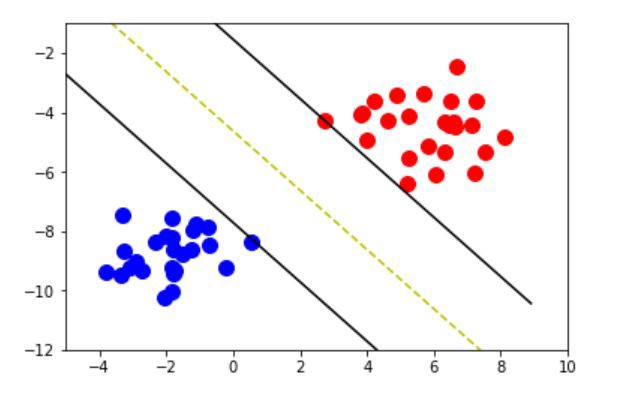
\includegraphics[width=14cm]{images/svm.jpeg}
			\end{figure} \\
			\hline
		\end{tabular}
	\end{adjustbox}
	\captionof{figure}{Contoh \textit{Hyperplane} pada SVM}
	\label{fig:hyperplanesvm}
\end{table}

\noindent SVM pada mulanya digunakan untuk menangani klasifikasi yang terdiri dari 2 kelas saja. Namun seriring dengan perkembangan zaman masalah yang dihadapi semakin kompleks sehingga membutuhkan teknik untuk melakukan proses klasifikasi lebih dari 2 kelas. Untuk melakukan klasifikasi lebih dari 2 kelas, terdapat 2 pendekatan yang bisa digunakan yaitu \textit{One-Versus-One} dan \textit{One-Versus-Rest}. Pada pendekatan \textit{One-Versus-One}, akan dibuat sebanyak $k(k-1)/2$  pasangan kelas untuk pengujian untuk klasifikasi dengan kelas sebanyak $k$. Untuk menentukan kelas mana yang menjadi klasifikasi untuk suatu kumpulan data caranya adalah sistem \textit{voting}. Kelas dengan jumlah \textit{voting} terbanyak akan menjadi \textit{classifier} untuk data tersebut. Pada pendekatan \textit{One-Versus-Rest} akan dibuat sebanyak $k$ pasangan kelas untuk klasifikasi dengan kelas sebanyak $k$. Setiap kelas yang diuji akan dibandingkan dengan sisa kelas yang ada. Misal terdapat 3 kelas A,B, dan C, maka kelas A akan dibandingkan dengan kelas B dan C, kelas B dibandingkan dengan kelas A dan C, kelas C dibandingkan dengan kelas A dan B. Kekurangan dari pendekatan ini adalah jumlah \textit{training set} yang tidak seimbang \cite{svm}.

\noindent Untuk proses klasifikasi \textit{non-linear} dapat dicari dengan persamaan 2.13 berikut:
\begin{table}[H]
	\small
	\begin{adjustbox}{width=1\textwidth}
		\begin{tabular}{|p{13.55cm}|}
			\hline
			\begin{equation}
			f(x) = sign(\sum_{i=1}^{l}\alpha_iy_iK(x,x_i)+b)
			\end{equation}\\
			\hline
		\end{tabular}
	\end{adjustbox}
\end{table}
\noindent
\renewcommand{\arraystretch}{1} 
\begin{tabularx}{\textwidth}{lll}
	Dimana: \\
	$l$ & = & Banyaknya kelas citra\\
	$\alpha_i$ & = & Nilai alpha ke $i$\\
	$y_i$ & = & Nilai kelas citra ke $i$\\
	$K(x,x_i)$ & = & Fungsi kernel\\
	$b$ & = & Nilai bias\\
\end{tabularx}

\noindent Nilai $\alpha$ dan $b$ dapat dicari dengan persamaan linear yang membentuk \textit{hyperplane} SVM. Persamaan \ref{eq:PersamaanSVM1} sampai \ref{eq:PersamaanSVM2} berikut merupakan persamaan \textit{hyperplane} SVM:

\begin{table}[H]
	\small
	\begin{adjustbox}{width=1\textwidth}
		\begin{tabular}{|p{13.55cm}|}
			\hline
			\begin{equation}
			\sum_{i=1}^{l}\alpha_iy_iK(x,x_i)+b)=0
			\label{eq:PersamaanSVM1}
			\end{equation}
			\begin{equation}
			\sum_{i=1}^{l}\alpha_iy_iK(x,x_i)+b)=1
			\end{equation}
			\begin{equation}
			\sum_{i=1}^{l}\alpha_iy_iK(x,x_i)+b)=-1
			\label{eq:PersamaanSVM2}
			\end{equation}\\
			\hline
		\end{tabular}
	\end{adjustbox}
\end{table}
\noindent
\renewcommand{\arraystretch}{1} 
\begin{tabularx}{\textwidth}{lll}
	Dimana: \\
	$l$ & = & banyaknya kelas citra\\
	$\alpha_i$ & = & nilai alpha ke $i$\\
	$y_i$ & = & nilai kelas citra ke $i$\\
	$K(x,x_i)$ & = & fungsi kernel\\
	$b$ & = & nilai bias\\
\end{tabularx}

\noindent Seringkali kasus yang ada dalam dunia nyata tidak selalu bisa dipisahkan secara linier (\textit{linearly separable}) seperti pada contoh gambar di atas. Misalnya suatu kumpulan data memiliki fitur yang memiliki n-dimensi. Linear SVM tidak bisa diterapkan untuk kasus tersebut, sehingga diperlukan teknik agar membuat \textit{hyperplane} yang bisa memisahkan antara 2 kelas dalam ruang multidimensi. Cara yang umum digunakan untuk menyelesaikan masalah tersebut adalah dengan menggunakan kernel. Kernel yang umum digunakan pada SVM yaitu \textit{Radial Basis Function} seperti pada persamaan \ref{eq:PersamaanRBF} berikut:

\begin{table}[H]
	\small
	\begin{adjustbox}{width=1\textwidth}
		\begin{tabular}{|p{13.55cm}|}
			\hline
			\begin{equation}
			RBF = K(x_i,x_j) = \exp (-\frac{\|x_i-x_j\|}{2\sigma^2})
			\label{eq:PersamaanRBF}
			\end{equation}\\
			\hline
		\end{tabular}
	\end{adjustbox}
\end{table}
\noindent
\renewcommand{\arraystretch}{1} 
\begin{tabularx}{\textwidth}{lll}
	Dimana: \\
	$K$ & = & nilai fungsi kernel RBF\\
	$x_i$ & = & vektor input 1\\
	$x_j$ & = & vektor input 2\\
	$\sigma$ & = & konstanta sigma\\
\end{tabularx}
\vspace{4.5pt}

\subsection{\textit{Confusion Matrix}}
\noindent \textit{Confusion Matrix} merupakan metode pengukuran untuk mengevaluasi hasil klasifikasi. Dengan melakukan klasifikasi sebanyak $C$ kelas, dihasilkan \textit{confusion matrix} $M$ berukuran $C \times C$, di mana elemen $M_{ij}$ dalam matriks menunjukkan jumlah sampel yang salah diklasifikasikan, sementara $M_{ii}$ adalah jumlah sampel yang hasil klasifikasinya adalah benar. \textit{Confusion matrix} pada gambar \ref{fig:ConfusionMatrix} digunakan pada kasus klasifikasi dua buah kelas sehingga membentuk matriks berukuran $2 \times 2$ \cite{markham}.

\begin{adjustbox}{width=1\textwidth}
\noindent\begin{minipage}{\linewidth}
	\framebox[\textwidth]{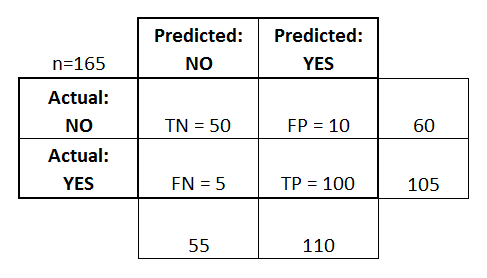
\includegraphics[width=8cm]{images/ConfusionMatrixForBinaryClassification.png}}
	\captionof{figure}{\textit{Confusion Matrix untuk Dua Kelas} \cite{markham}}
	\label{fig:ConfusionMatrix}
\end{minipage}
\end{adjustbox}

\noindent Elemen $M_{11}$ pada matriks menunjukkan jumlah sampel yang pada kenyataannya adalah kelas 1 dan diklasifikasikan sebagai kelas 1, sehingga disebut sampel \textit{true-positive} (TP). Elemen $M_{12}$ menunjukkan jumlah sampel yang pada kenyataannya adalah kelas 1 tetapi diklasifikasikan sebagai kelas -1, sehingga disebut sampel \textit{false-negative} (FN). Elemen $M_{21}$ menunjukkan jumlah sample yang pada kenyataannya adalah kelas -1 tetapi diklasifikasikan sebagai kelas 1, sehingga disebut sampel \textit{false-positive} (FP). Dan elemen $M_{22}$ menunjukkan jumlah sampel yang kenyataannya adalah kelas -1 dan diklasifikasikan sebagai kelas -1, sehingga disebut \textit{true-negative} (TN). Maka untuk menghitung akurasi dapat digunakan persamaan \ref{eq:accuracy}. Hasil akurasi yang semakin baik akan mendekati nilai 1, sebaliknya akurasi yang buruk mendekati nilai 0.
\begin{table}[H]
	\begin{adjustbox}{width=1\textwidth}
	\begin{tabular}{|p{13.55cm}|}
		\hline
		\begin{equation}
			Accuracy = \frac{TP + TN}{TP + TN + FP + FN}
			\label{eq:accuracy}
		\end{equation}\\
	\hline
	\end{tabular}
	\end{adjustbox}
\end{table}

Lalu perhitungan \textit{precision} yang merupakan perbandingan dari hasil positif dapat dihitung dengan persamaan \ref{eq:precision}.
\begin{table}[H]
	\begin{adjustbox}{width=1\textwidth}
	\begin{tabular}{|p{13.55cm}|}
		\hline
		\begin{equation}
			Precision = \frac{TP}{TP + FP}
			\label{eq:precision}
		\end{equation}\\
	\hline
	\end{tabular}
	\end{adjustbox}
\end{table}

Dan perhitungan \textit{recall} atau disebut juga sebagai sensitivitas dapat dihitung dengan persamaan \ref{eq:recall}.
\begin{table}[H]
	\begin{adjustbox}{width=1\textwidth}
	\begin{tabular}{|p{13.55cm}|}
		\hline
		\begin{equation}
			Recall = \frac{TP}{TP + FN}
			\label{eq:recall}
		\end{equation}\\
	\hline
	\end{tabular}
	\end{adjustbox}
\end{table}

\subsection{Penggunaan \textit{Library}}
\noindent Berikut adalah penjelasan dari \textit{library} yang digunakan di dalam penelitian. \\
\subsubsection{OpenCV}
\noindent\textit{Library} yang digunakan adalah OpenCV untuk proses \textit{pre-processing} citra. OpenCV merupakan \textit{library open-source} yang banyak digunakan untuk penelitian terkait proses pengolahan citra dan \textit{computer vision}. 
\begin{small}
	\begin{longtable}{| p {0.5cm} | p {6cm} | p {6cm} |}
		\caption{Tabel fungsi \textit{Library} OpenCV} \\
		\hline
		\textbf{No}  & \textbf{\textit{Function}}  & \textbf{Deskripsi} \\
		\hline
		\endfirsthead
		\endhead
		1 & Imgcodecs.imread(String filename) & Mengambil citra dari \textit{path} yang diisikan ke parameter.\\
		\hline
		2 & Imgproc.cvtColor(Mat src, Mat dst, int code) & Mengubah jenis warna pada citra sesuai yang diinginkan. Parameter fungsi ini terdiri dari Mat asal, Mat tujuan, dan \textit{code}. \textit{Code} digunakan untuk memilih tipe konversi citra tersebut, misal \textit{grayscale}.\\
		\hline
		3 & Imgproc.Canny(Mat image,Mat edges,double threshold1, double threshold2) & Fungsi ini digunakan untuk mendeteksi tepian pada citra menggunakan Canny.\\
		\hline
	\end{longtable}
\end{small}
\subsubsection{Weka}
\noindent Weka adalah kumpulan dari algoritme pembelajaran mesin yang digunakan untuk menyelesaikan permasalahan \textit{data mining}. \textit{Library} ini berbasis bahasa pemrograman Java dan dapat berjalan di hampir seluruh platform. Dalam penelitian ini, \textit{library} Weka digunakan untuk melakukan proses klasifikasi menggunakan metode \textit{Support Vector Machine}.
\begin{small}
	\begin{longtable}{| p {0.5cm} | p {6cm} | p {6cm} |}
		\caption{Tabel fungsi \textit{Library} Weka} \\
		\hline
		\textbf{No}  & \textbf{\textit{Function}}  & \textbf{Deskripsi} \\
		\hline
		\endfirsthead
		\endhead
		1 & libsvm.setOptions(String options) & Mengkonfigurasi \textit{classifier} yang akan digunakan.\\
		\hline
		2 & libsvm.buildClassifier(Instances insts) & Membangun \textit{classifier} sesuai dengan konfigurasi yang digunakan dan dataset yang diberikan.\\
		\hline
	\end{longtable}
\end{small}

\section{Tinjauan Studi}
\noindent Pada bagian ini akan dijelaskan mengenai perbandingan dari berbagai penelitian terkait metode deteksi dan pengenalan plat nomor mobil. \\

\subsection{\textit{State of the Art}}
\noindent Terdapat beberapa metode lain yang memiliki ruang lingkup yang mirip dengan penelitian ini khususnya mengenai deteksi dan pengenalan plat nomor mobil. Tabel \ref{tbl:StateoftheArt} \textit{State of the Art} akan menjelaskan perbedaan-perbedaan metode dari jurnal terkait.\\
\\
\\
\\
\\
\\
\\
\\
\\
\begingroup
\setlength{\LTleft}{-20cm plus -1fill}
\setlength{\LTright}{\LTleft}
\begin{small}
\begin{longtable}{ |p{5cm}|p{3.5cm}|p{3.6cm}| }
\caption{\textit{State of the Art}}\\
\hline
\textbf{Jurnal} & \textbf{Rumusan Masalah} & \textbf{Metode}\\
\endfirsthead

\multicolumn{3}{c}{\textbf{\tablename~\thetable} \textit{State of the Art} (Lanjutan)}\\
\hline
\textbf{Jurnal} & \textbf{Rumusan Masalah} & \textbf{Metode}\\
\endhead

\hline
 Gou, C., Wang, K., Yao, Y., Li, Z. (2016). Vehicle license plate recognition based on extremal regions and restricted Boltzmann machines. \emph{IEEE Transactions on Intelligent Transportation Systems, 17}(4), 1096-1107. & Apakah dengan menerapkan pendeteksian plat nomor dengan \textit{Extremal Region} dan pengenalan karakter plat nomor menggunakan \textit{Hybrid Discriminative Restricted Boltzmann Machine} dapat meningkatkan akurasi pendeteksian dan pengenalan dalam berbagai kondisi cuaca dan \textit{background} yang kompleks? & 
\begin{enumerate}[wide, labelwidth=!, labelindent=0pt, topsep=0pt]
\item \textit{Extremal Region}
\item \textit{AdaBoost}
\item \textit{Histogram of Oriented Gradient}
\item \textit{Hybrid Discriminative Restricted Boltzmann Machine} 
\end{enumerate}\\
\hline
 Gou, C., Wang, K., Yu, Z., Xie, H. (2014, October). License plate recognition using MSER and HOG based on ELM. In \emph{Proceedings of 2014 IEEE International Conference on Service Operations and Logistics, and Informatics} (pp. 217-221). IEEE. & Apakah dengan menerapkan \textit{Maximally Stable Extremal Region} untuk pendeteksian plat nomor dan \textit{Extreme Learning Machine} untuk pengenalan karakter plat nomor dapat meningkatkan performa dan akurasi sistem? & 
\begin{enumerate}[wide, labelwidth=!, labelindent=0pt, topsep=0pt]
\item \textit{Maximally Stable Extremal Region}
\item \textit{Histogram of Oriented Gradient}
\item \textit{Extreme Learning Machine}
\end{enumerate}\\
\hline
Tabrizi, S. S., Cavus, N. (2016). A hybrid KNN-SVM model for Iranian license plate recognition. \emph{Procedia Computer Science, 102}, pp. 588-594. & Apakah dengan menggabungkan metode klasifikasi \textit{K-Nearest Neighbours} dan \textit{Support Vector Machine} akan menghasilkan akurasi yang lebih baik dan mengurangi \textit{cost} pada proses pengenalan karakter plat nomor kendaraan? &
\begin{enumerate}[wide, labelwidth=!, labelindent=0pt, topsep=0pt]
\item \textit{Structural Feature}
\item \textit{Horizontal and Vertical Crossing Count Histogram}
\item \textit{Zoning Feature Extraction}
\item \textit{K-Nearest Neigbhours}
\item \textit{Support Vector Machine}
\end{enumerate}\\
\hline
Rasheed, S., Naeem, A., Ishaq, O. (2012, October). Automated number plate recognition using hough lines and template matching. In \emph{Proceedings of the World Congress on Engineering and Computer Science} (Vol. 1, pp. 24-26). & Apakah dengan menggunakan metode \textit{Hough Transform} untuk mendeteksi plat kendaraan dan \textit{Template Matching} untuk pengenalan karakter dapat menghasilkan akurasi yang baik untuk sistem pengenalan plat nomor kendaraan? &
\begin{enumerate}[wide, labelwidth=!, labelindent=0pt, topsep=0pt]
	\item \textit{Canny Detector}
	\item \textit{Hough Transform}
	\item \textit{Morphological Process}
	\item \textit{Template Matching}
\end{enumerate}\\
\hline
Nugroho, A., Wardhani, K.R.R. (2011). Aplikasi Sistem Pembaca Plat Nomor Mobil Menggunakan Pengolahan Citra dan Metode Learning Vector Quantization. & Apakah dengan menerapkan pengolahan citra untuk deteksi plat kendaraan dan metode \textit{Learning Vector Quantization} untuk pengenalan karakter dapat menghasilkan akurasi yang baik ? &
\begin{enumerate}[wide, labelwidth=!, labelindent=0pt, topsep=0pt]
	\item \textit{Pengolahan Citra}
	\item \textit{Learning Vector Machine}
\end{enumerate}
\label{tbl:StateoftheArt}\\
\hline
\end{longtable}
\end{small}
\endgroup
 
\subsection{Pembahasan Penelitian Terkait}
\noindent Terdapat beberapa metode yang dapat khususnya untuk mendeteksi plat nomor dan mengenali karakter pada plat nomor.
\noindent Pada referensi pertama \cite{gou2016} menggunakan metode \textit{Extremal Region} sebagai proses untuk mendapatkan daerah-daerah karakter dari suatu plat nomor, kemudian \textit{Extremal Region} yang didapat diseleksi dengan menggunakan \textit{AdaBoost} sehingga bisa didapatkan daerah karakter plat nomor yang sesuai dengan kriteria yang diinginkan, dari daerah-daerah karakter yang didapatkan barulah kandidat plat nomor yang benar bisa didapatkan. Proses selanjutnya adalah pengambilan fitur karakter dengan menggunakan metode \textit{Histogram of Oriented Gradient} sehingga didapatkan fitur vektor dari setiap karakter pada plat nomor, yang nantinya akan menjadi masukkan bagi metode klasifikasi \textit{Hybrid Discriminative Restricted Boltzmann Machine}.

\noindent Pada referensi kedua \cite{gou2014} menggunakan metode \textit{Maximally Stable Extremal Region} untuk memilih kandidat daerah karakter yang nantinya akan menentukan lokasi dari plat nomor berdasarkan letak geometris dari kandidat-kandidat karakter tersebut. Setelah lokasi plat nomor didapatkan, \textit{HOG Descriptor} dari setiap karakter diambil dengan menggunakan metode \textit{Histogram of Oriented Gradient} dan setiap karakternya akan dikenali menggunakan metode \textit{neural network} bernama \textit{Extreme Learning Machine}.

\noindent Pada referensi ketiga \cite{tabrizi} digabungkan metode klasifikasi \textit{K-Nearest Neighbours} dengan metode klasifikasi \textit{Support Vector Machine}. \textit{K-Nearest Neighbours} digunakan karena sifatnya yang mudah dipelajari, bersifat tangguh terhadap data yang memiliki derau dan efektif jika jumlah yang dimiliki berjumlah banyak. Sedangkan metode \textit{Support Vector Machine} digunakan untuk karakter-karakter yang memiliki kemiripan karakteristik, sehingga akurasi dari pengenalan karakter dapat meningkat.

\noindent Pada referensi keempat \cite{rasheed} menggunakan \textit{Hough Transform} untuk mendeteksi lokasi plat kendaraan dan menghasilkan akurasi yang baik, yaitu sekitar 94\% untuk plat nomor yang terdeteksi dan dengan menggunakan metode \textit{Template Matching} menghasilkan akurasi pengenalan karakter plat nomor kendaraan sebesar 90\%.

\noindent Pada referensi kelima \cite{nugroho} menggunakan metode pengolahan citra untuk mencari kandidat-kandidat pita dengan menghitung histogram gambar untuk mendapatkan lokasi plat nomor kendaraan, kemudian setiap karakter dari plat nomor yang didapatkan disegmentasi dengan cara menghitung grafik horizontal gambar, kemudian untuk metode klasifikasi karakter yang digunakan adalah \textit{Learning Vector Quantization}.\\

\section{Tinjauan Objek}
\noindent Pada bagian ini akan diulas mengenai objek-objek yang terkait dengan deteksi dan pengenalan plat nomor kendaraan.\\

\subsection{Tanda Nomor Kendaraan Bermotor}
\noindent Tanda Nomor Kendaraan Bermotor (disingkat TNKB) disebut juga sebagai plat nomor atau nomor polisi adalah plat aluminium tanda kendaraan bermotor di Indonesia yang telah didaftarkan pada Kantor Bersama Samsat.

\begin{adjustbox}{width=1\textwidth}
\noindent\begin{minipage}{\linewidth}
	\centering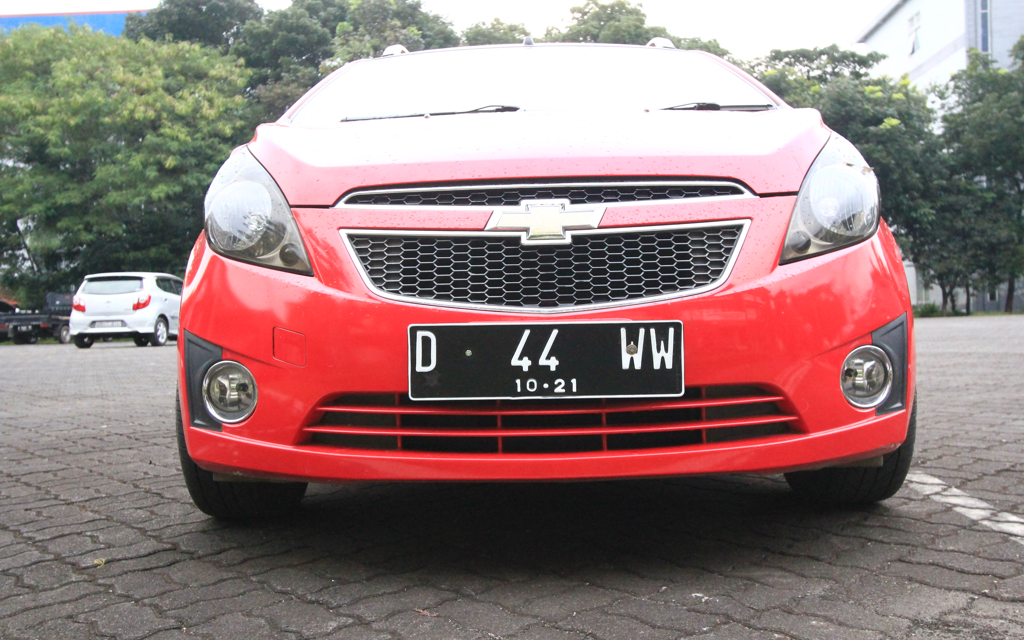
\includegraphics[width=12cm]{images/plat_nomor_example.png}
	\captionof{figure}{Contoh dari plat nomor kendaraan Indonesia}
	\label{fig:ContohPlatNomorIndonesia}
\end{minipage}
\end{adjustbox}\\

\subsection{Spesifikasi Teknis}
\noindent Plat nomor kendaraan Indonesia terdiri dari cetakan tulisan dua baris, pada baris pertama terdapat tiga hal yang diinformasikan, yaitu kode wilayah(huruf), nomor polisi(angka), dan kode/seri akhir wilayah(huruf). Sedangkan baris kedua menunjukkan bulan dan tahun masa berlaku, masing-masing dua digit. Contohnya pada gambar \ref{fig:ContohPlatNomorIndonesia} angka yang terdapat di baris keduanya adalah 10.21. Hal tersebut menandakan bahwa plat nomor tersebut akan habis masa berlakunya pada bulan Oktober tahun 2021.

\noindent Bahan baku dari plat nomor adalah aluminium dengan ketebalan 1mm. Ukuran plat nomor untuk kendaraan bermotor roda dua dan roda tiga adalah 250 $\times$ 105 mm, sedangkan untuk kendaraan bermotor roda empat atau lebih adalah 395 $\times$ 135 mm. Terdapat cetakan garis lurus pembatas selebar 5mm di antara ruang nomor polisi dengan ruang angka masa berlaku (untuk plat nomor lama), sedangkan semenjak tahun 2011 di sekitar plat nomor terdapat garis putih dan tidak ada garis pemisah antara nomor polisi dan masa berlaku.

\noindent Pada tahun 2014 terjadi perubahan tampilan pada plat nomor untuk kendaraan bermotor roda empat. Plat nomor kini sedikit lebih panjang dari sebelumnya (5 cm lebih panjang) untuk memberi ruang pada kode/seri akhir wilayah yang dulunya berjumlah dua digit menjadi tiga digit.\\

\subsection{Jenis TNKB}
\noindent Jenis dari TNKB di Indonesia dibedakan berdasarkan warna dari TNKB tersebut, warna TNKB yang ditetapkan di Indonesia adalah sebagai berikut:
\begin{enumerate}
\item Kendaraan pribadi dan sewa: warna dasar hitam dengan tulisan berwarna putih.
\item Kendaraan umum: warna dasar kuning dengan tulisan hitam.
\item Kendaraan milik pemerintah: warna dasar merah dengan tulisan berwarna putih.
\item Kendaraan bermotor sementara: warna dasar putih dengan tulisan berwarna merah.
\item Kendaraan korps diplomatik negara asing: warna dasar putih/merah dengan tulisan berwarna hitam.
\item Kendaraan staf operasional korps diplomatik negara asing: warna dasar hitam dengan tulisan berwarna putih serta terdiri dari lima angka dan kode angka negara yang dicetak lebih kecil dengan format sub-bagian.
\end{enumerate}

%\subsubsection{Pendeteksian dan Pelacakan Manusia}
%\noindent Pada bagian ini akan dijelaskan beberapa teori mengenai deteksi manusia dan pelacakan manusia.\\

%\subsubsection{Deteksi dan Melacak Manusia}
%\noindent Pendeteksian manusia adalah proses atau tahap awal untuk menemukan dan menentukan posisi objek manusia dari sebuah citra. Pendeteksian manusia ini fokus untuk menemukan bagian atas badan manusia dari tampak depan maupun tampak belakang, seperti yang terlihat pada gambar \ref{fig:ContohDeteksiManusia}. Sementara pelacakan manusia adalah proses untuk mengikuti jejak pergerakan dari objek manusia yang telah terdeteksi pada tahap sebelumnya. Tahap ini menggunakan estimasi perubahan atau pergerakan sehingga tidak perlu terus-menerus melakukan proses pendeteksian manusia pada setiap citra.\\
%\begin{adjustbox}{width=1\textwidth}
%\noindent\begin{minipage}{\linewidth}
%	\framebox[\textwidth]{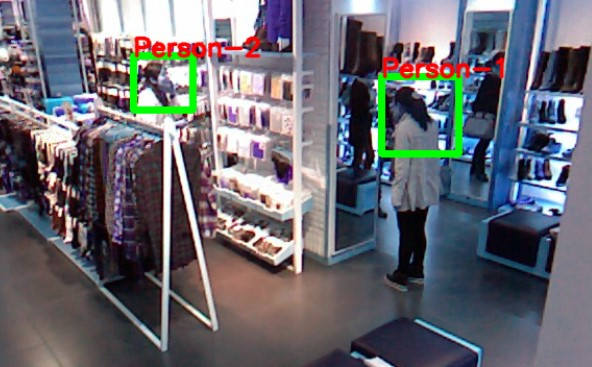
\includegraphics[width=8cm]{images/DeteksiManusia.jpg}}
%	\captionof{figure}{Contoh dari pendeteksian manusia \cite{15}}
%	\label{fig:ContohDeteksiManusia}
%\end{minipage}
%\end{adjustbox}\\

%\subsection{\textit{Database RGB-D}}
%\noindent \textit{Database RGB-D} didapatkan dari \textit{Fudan University}. \textit{Fudan University} memiliki dan menyediakan \textit{database} yang dapat digunakan secara gratis oleh umum. Dalam penelitian ini digunakan 2 buah \textit{dataset} positif yang terdapat manusia di dalamnya, ditangkap oleh \textit{Fudan University} menggunakan sensor Microsoft Kinect yang memiliki resolusi berukuran 640 $\times$ 480 dengan \textit{frame rate} 30 fps. Sensor yang digunakan Microsoft Kinect dapat menangkap sepasang citra dalam waktu bersamaan yaitu citra RGB dan citra kedalaman sehingga menjadi citra RGB-D.

%\noindent Dalam masing-masing \textit{dataset} terdapat sepasang kumpulan citra yaitu citra tipe RGB dan citra kedalaman. Selain itu, diberitahukan juga koordinat \textit{ground truth} pada setiap pasangan citra yang menandakan posisi manusia yang terdapat pada citra tersebut.
%\textit{Dataset} yang pertama bernama \textit{Clothing Store RGBD}, berada pada salah satu toko pakaian dengan jumlah citra 1.000 buah untuk masing-masing tipe citra. Dalam 1.000 citra tersebut terdapat 2.367 posisi manusia pada berkas \textit{ground truth}. Contoh sepasang citra yang terdapat pada \textit{dataset} pertama dapat dilihat pada gambar \ref{fig:DatasetClothingStore}, di mana seharusnya terdapat 2 orang yang terdeteksi. \\
%\begin{adjustbox}{width=1\textwidth}
%\noindent\begin{minipage}{\linewidth}
%	\framebox[\textwidth]{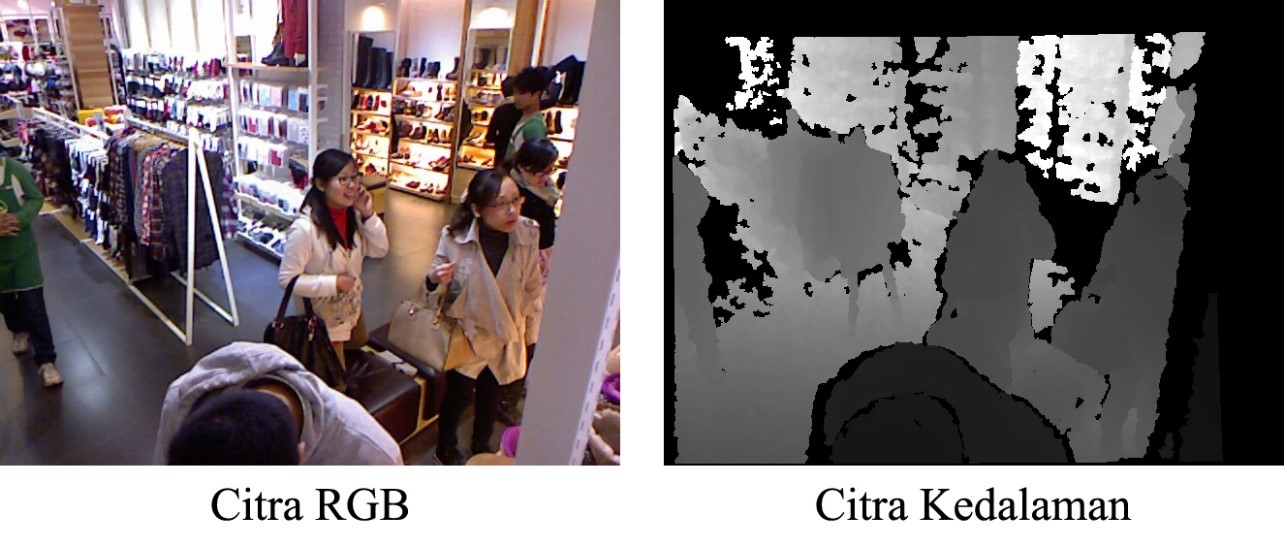
\includegraphics[width=12cm]{images/DBClothingStore.jpg}}
%	\captionof{figure}{\textit{Dataset} CLOTHING STORE \cite{15}}
%	\label{fig:DatasetClothingStore}
%\end{minipage}
%\end{adjustbox}\\

%\noindent Pada gambar \ref{fig:GroundTruthClothingStore} terlihat \textit{ground truth} dari setiap citra \textit{dataset Clothing Store}, di mana angka awal sebelum titik dua merupakan citra pada waktu \textit{fps} tertentu dan setiap kurung siku menyatakan keberadaan posisi manusia pada citra, yang masing-masing terdiri atas $x_{1},y_{1}$ untuk koordinat titik kiri atas dan $x_{2},y_{2}$ untuk koordinat titik kanan bawah. \\
%\begin{adjustbox}{width=1\textwidth}
%\noindent\begin{minipage}{\linewidth}
%	\framebox[\textwidth]{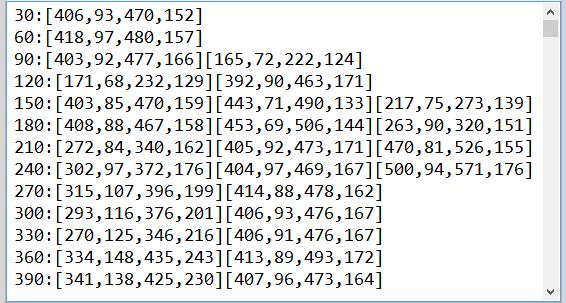
\includegraphics[width=8cm]{images/GroundTruthClothingStore.jpg}}
%	\captionof{figure}{Berkas \textit{ground truth} CLOTHING STORE \cite{15}}
%	\label{fig:GroundTruthClothingStore}
%\end{minipage}
%\end{adjustbox}\\

%\noindent Untuk dataset kedua bernama \textit{Outdoor crowds in the dark RGBD}, berada di lingkungan \textit{Fudan University} pada malam hari sehingga kondisi pencahayaannya relatif redup dengan jumlah citra total adalah 275 buah untuk masing-masing tipe citra. Berbeda dengan \textit{dataset} pertama, pada \textit{dataset Outdoor} terdapat tiga buah folder bernama 31, 54, dan 56. Jumlah citra pada masing-masing folder bervariasi dan telah dilengkapi dengan berkas \textit{ground truth}. Penjelasan lebih rinci mengenai \textit{dataset} ini dapat dilihat pada tabel \ref{tbl:Outdoor}.
%\begin{table}[H]
%\centering
%\begin{small}
%\captionof{table}{Rincian \textit{Dataset Outdoor} \label{tbl:Outdoor}}
%\begin{tabular}{|p{1cm}|p{3cm}|p{3cm}|}
%	\hline
%	\textbf{Folder} & \textbf{Jumlah Citra} & \textbf{Jumlah Posisi Manusia}\\
%	\hline
%	31 & 57 & 273 \\
%	\hline
%	54 & 95 & 427 \\
%	\hline
%	56 & 123 & 548 \\
%	\hline
%\end{tabular}
%\end{small}
%\end{table}

%\noindent Contoh sepasang citra yang terdapat pada dataset kedua dapat dilihat pada gambar \ref{fig:DatasetOutdoor}, di mana seharusnya terdapat 6 orang yang terdeteksi. \\
%\begin{adjustbox}{width=1\textwidth}
%\noindent\begin{minipage}{\linewidth}
%	\framebox[\textwidth]{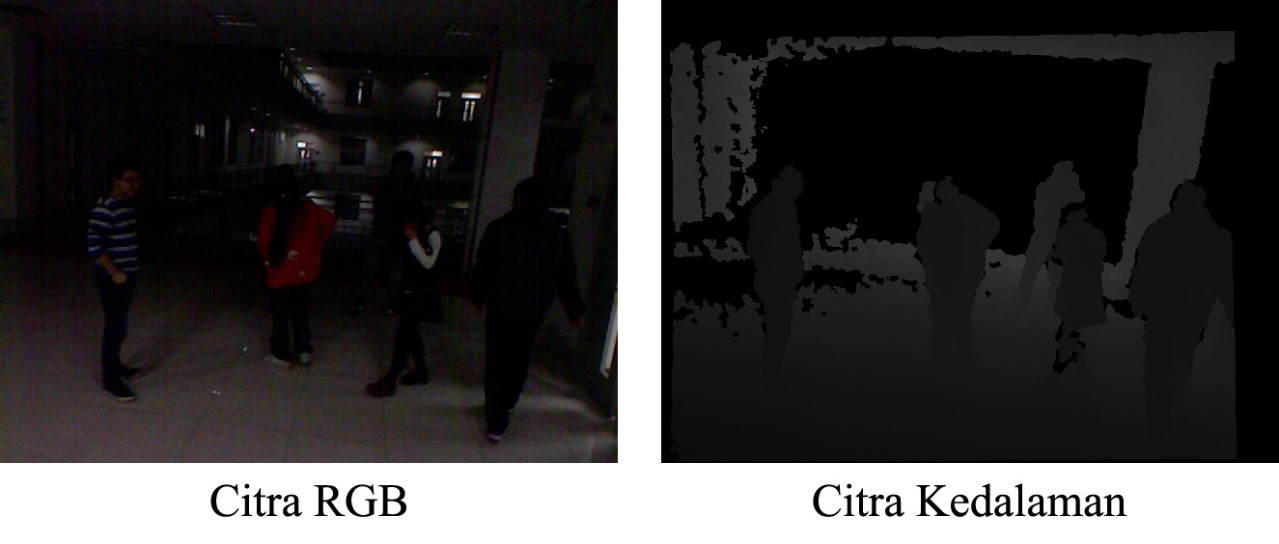
\includegraphics[width=12cm]{images/DBOutdoor.jpg}}
%	\captionof{figure}{\textit{Dataset} OUTDOOR \cite{15}}
%	\label{fig:DatasetOutdoor}
%\end{minipage}
%\end{adjustbox}\\

%\noindent Pada gambar \ref{fig:GroundTruthOutdoor} terlihat \textit{ground truth} dari setiap citra \textit{dataset Outdoor}, di mana nilai yang berada dalam tanda kutip dua merupakan lokasi dengan nama citra dan setiap nilai di dalam tanda kurung menyatakan keberadaan posisi manusia pada citra, yang masing-masing terdiri atas $x_{1},y_{1}$ untuk koordinat titik kiri atas dan $x_{2},y_{2}$ untuk koordinat titik kanan bawah. \\
%\begin{adjustbox}{width=1\textwidth}
%\noindent\begin{minipage}{\linewidth}
%	\framebox[\textwidth]{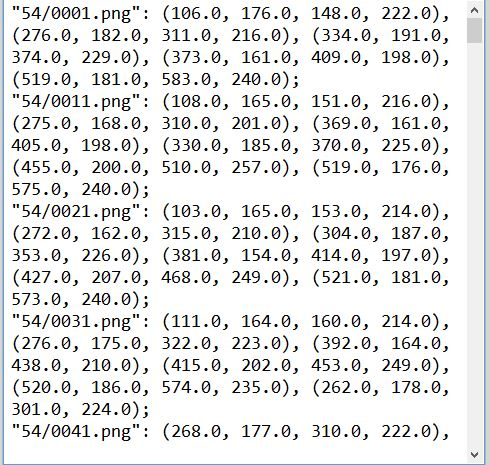
\includegraphics[width=8cm]{images/GroundTruthOutdoor.jpg}}
%	\captionof{figure}{Berkas \textit{ground truth} OUTDOOR \cite{15}}
%	\label{fig:GroundTruthOutdoor}
%\end{minipage}
%\end{adjustbox}\\

%\noindent \textit{Dataset} pertama akan dibagi dengan perbandingan 80:20, 80\% akan digunakan sebagai \textit{data training} dan 20\% digunakan sebagai {data testing}. Untuk \textit{dataset} kedua, folder 56 akan digunakan sebagai \textit{data training} dan folder 31 dan 54 digunakan sebagai {data testing}. \textit{Dataset} negatif yang tidak mengandung manusia akan diambil secara acak berukuran 65 $\times$ 80 dari masing-masing \textit{dataset} dengan ketentuan, tidak berpotongan dengan posisi \textit{ground truth}.

\newpage
	\setcounter{page}{1}
	%-----------------------------------------------------------------------------%
\chapter{ANALISIS DAN PERANCANGAN SISTEM}
%-----------------------------------------------------------------------------%

%
\vspace{4.5pt}

\noindent Bab ini memaparkan analisis masalah yang diatasi berserta pendekatan dan alur kerja dari perangkat lunak yang dikembangkan, mengimplementasikan metode yang digunakan dan hasil yang akan ditampilkan.
\\
\section{Analisis Masalah}
\noindent Pada bab 1 telah dijelaskan bahwa penelitian mengenai sistem pengenalan plat nomor kendaraan merupakan bidang yang masih berkembang dan implementasinya memegang peranan penting dalam bidang transportasi. Pada penelitian ini, metode yang akan digunakan adalah \textit{Hough Transform} untuk mendeteksi lokasi plat kendaraan, kemudian menggunakan metode \textit{Histogram of Oriented Gradient} untuk mengekstraksi fitur dari citra karakter dari plat nomor yang sudah disegmentasi dengan menghitung grafik horizontal pita, kemudian dilakukan klasifikasi dengan menggunakan metode \textit{Support Vector Machine}.
\noindent Masukan untuk sistem deteksi dan pengenalan plat nomor kendaraan ini adalah citra yang ditangkap oleh kamera DSLR Canon EOS 500 D dan Canon EOS 550 D beresolusi 15 dan 18 megapiksel. Citra tangkapan kemudian akan diubah resolusinya menjadi 1024 $\times$ 640 piksel. Setiap citra masukan berisi bagian depan dari kendaraan yang memiliki plat nomor kendaraan.
\noindent Keluaran atau hasil dari sistem akan berupa teks hasil dari pengenalan karakter pada citra plat nomor kendaraan masukan.\\ 

\section{Kerangka Pemikiran}
\noindent Berikut ini adalah kerangka pemikiran dari metode yang diusulkan untuk melakukan deteksi plat nomor kendaraan dan melakukan pengenalan karakter pada citra karakter yang terdapat pada plat nomor.
\\
\begin{adjustbox}{width=1\textwidth}
	\noindent
	\begin{minipage}{\linewidth}
		\framebox[\textwidth]{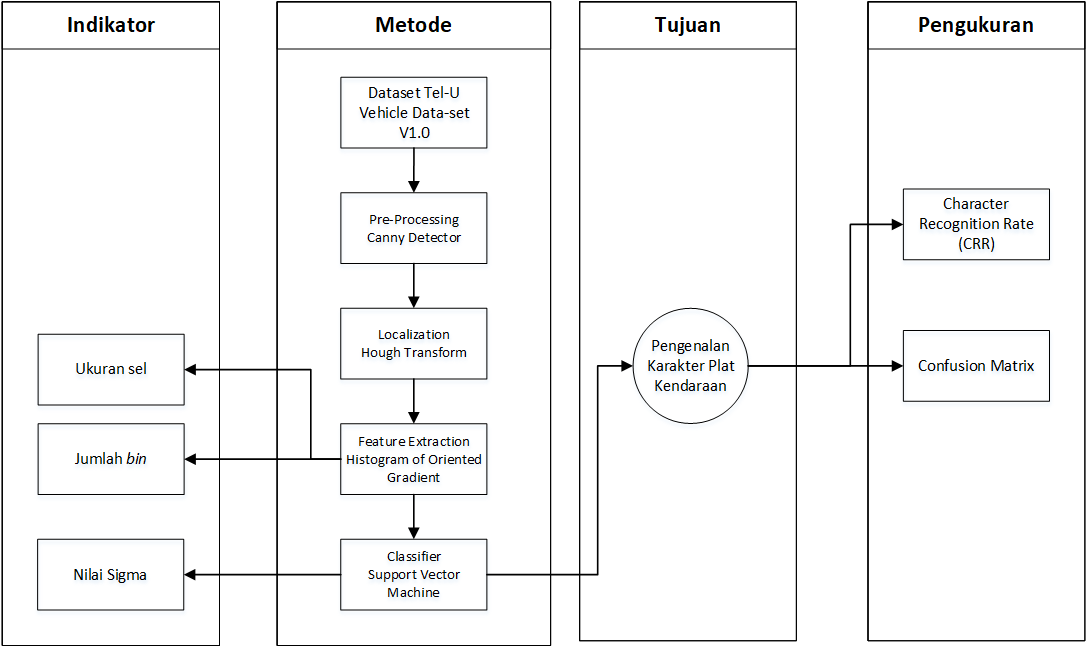
\includegraphics[width=13cm]{images/KerangkaPemikiran.png}}
		\captionof{figure}{Kerangka Pemikiran}
		\label{fig:KerangkaPemikiran}
	\end{minipage}
\end{adjustbox}

\noindent Seperti pada Gambar \ref{fig:KerangkaPemikiran}, terdapat beberapa variabel indikator yang mempengaruhi hasil dan perlu dilakukan penyesuaian, seperti ukuran sel pada metode \textit{Histogram of Oriented Gradient}, jumlah \textit{bin} yang menentukan batasan sudut yang digunakan, dan nilai sigma untuk \textit{classifier} \textit{Support Vector Machine}. Penelitian ini memiliki tujuan untuk menerapkan \textit{Histogram of Oriented Gradient} dan \textit{Support Vector Machine} untuk sistem pengenalan karakter pada plat nomor dengan menguji beragam faktor yang diduga akan mempengaruhi hasil akurasi dari penggabungan kedua metode tersebut. Hasil pengenalan karakter akan diukur dengan menggunakan \textit{Confusion Matrix}.\\

\section{Urutan Proses Global}
\noindent Dalam sistem pengenalan plat nomor kendaraan terbagi atas dua proses yaitu proses \textit{training} dan proses \textit{testing}. Proses \textit{training} dilakukan untuk mendapatkan kelas-kelas dari karakter-karakter yang akan dikenali. Proses \textit{testing} dilakukan untuk menghitung hasil yang berupa akurasi dari pengenalan karakter pada plat nomor kendaraan.\\

\begin{adjustbox}{width=1\textwidth}
	\noindent
	\begin{minipage}{\linewidth}
		\framebox[\textwidth]{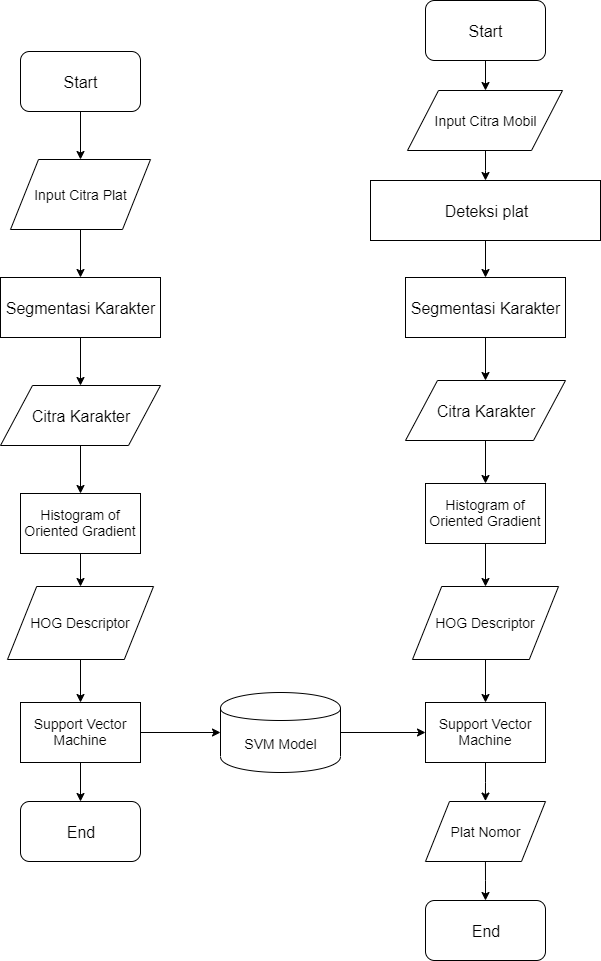
\includegraphics[width=12cm]{images/FlowchartGlobal.png}}
		\captionof{figure}{\textit{Flowchart Global} Sistem Pengenalan Plat Nomor Kendaraan\\}
		\label{fig:FlowchartGlobal}
	\end{minipage}
\end{adjustbox}

\noindent Seperti pada Gambar \ref{fig:FlowchartGlobal}. Bagian kiri merupakan \textit{flowchart} dari proses \textit{training} dan bagian kanan merupakan \textit{flowchart} dari proses \textit{testing}. Berikut ini adalah uraian dari proses-proses yang terjadi ketika tahapan \textit{training}:
\begin{enumerate}
	\item Citra masukan adalah citra plat nomor kendaraan mobil yang di-\textit{crop} secara manual dari citra mobil utuh hal ini untuk memastikan citra yang didapatkan adalah plat yang benar. 
	\item Citra plat kemudian akan melalui tahapan \textit{preprocessing} yang meliputi \textit{grayscaling} untuk menghilangkan informasi warna yang tidak diperlukan, \textit{Gaussian Smoothing} untuk menghilangkan derau pada citra, \textit{Binarization} untuk mengubah citra menjadi citra biner, menghilangkan objek kecil (untuk menghilangkan objek seperti baut pada plat) dengan cara menghilangkan objek yang luasnya kurang dari \textit{threshold} sebesar 100 piksel, dan terakhir \textit{Inverse Binarization} untuk mendapatkan citra karakter berwarna hitam dengan latar belakang berwarna putih.
	\item Citra plat selanjutnya melalui tahapan segmentasi karakter, tahapan segmentasi bertujuan untuk mendapatkan citra-citra karakter dari plat nomor tersebut tahapan segmentasi dilakukan dua tahapan, yaitu segmentasi horizontal dan segmentasi vertikal. Tahapan segmentasi dilakukan dengan menggunakan \textit{library} segmentasi dari \textit{JavaOCR}. Citra hasil segmentasi memiliki ukuran yang beragam, tetapi setiap citra diberi \textit{padding} sebesar 1 piksel dari tepian. Tujuannya agar bentuk objek bisa didapat dengan baik, hal ini akan membuat fitur yang didapat pada tahapan ekstraksi fitur menjadi lebih baik.
	\item Citra karakter hasil \textit{segmentasi} akan di-\textit{scaling} menjadi berukuran 32 $\times$ 32 piksel dengan tujuan untuk menyeragamkan ukuran citra karakter. Kumpulan karakter yang digunakan adalah karakter angka dari 0 sampai dengan 9 dan karakter huruf dari A sampai dengan Z, tidak ada karakter huruf kecil dikarenakan plat nomor kendaraan tidak ada yang menggunakan karakter huruf kecil.
	\item \textit{Histogram of Oriented Gradient} berfungsi untuk mendapatkan fitur dari citra hasil segmentasi. Hasil dari ekstraksi fitur dengan menggunakan HOG adalah \textit{HOG descriptor}, yang mendeskripsikan distribusi dari gradien berarah pada suatu area citra.
	\item Untuk ukuran sel dan jumlah \textit{bin} yang digunakan untuk proses ekstraksi fitur dengan menggunakan \textit{HOG}, dikarenakan kedua parameter tersebut merupakan indikator uji seperti ditunjukkan pada kerangka pemikiran \ref{fig:KerangkaPemikiran}, maka nilai dari ukuran sel dan jumlah \textit{bin} akan menyesuaikan dengan kondisi yang akan diuji.
	\item Setelah tahapan ekstraksi fitur, fitur-fitur akan disimpan dalam berkas CSV dan proses pelabelan fitur untuk setiap karakter akan dilakukan terhadap berkas CSV tersebut.
	\item \textit{Support Vector Machine} (SVM) digunakan untuk mengklasifikasikan fitur-fitur yang sudah didapatkan ke dalam kelas-kelas dari karakter yang akan dikenali. Metode \textit{SVM} yang digunakan pada penelitian ini berasal dari \textit{library WEKA}.
\end{enumerate}
%\subsection{Proses \textit{Training}}
%\begin{adjustbox}{width=1\textwidth}
%	\noindent
%	\begin{minipage}{\linewidth}
%		\framebox[\textwidth]{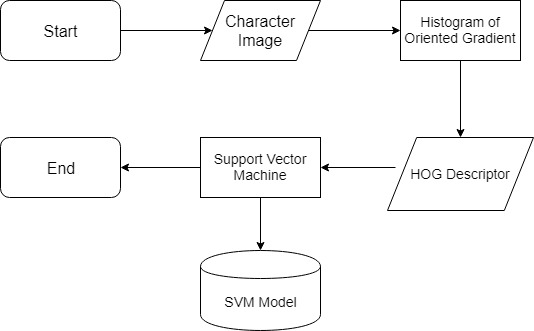
\includegraphics[width=12cm]{images/FlowchartTraining.jpg}}
%		\captionof{figure}{\textit{Flowchart Training} Sistem Pengenalan Plat Nomor Kendaraan\\}
%		\label{fig:FlowchartTraining}
%	\end{minipage}
%\end{adjustbox}
%Berikut ini adalah uraian dari \textit{flowchart} pada gambar \ref{fig:FlowchartTraining} yang dilakukan dalam penelitian ini:
%\begin{enumerate}
%	\item Citra yang menjadi masukkan adalah citra karakter hasil segmentasi dari citra plat nomor kendaraan. Citra karakter masukkan berukuran 32 $\times$ 32 piksel. Citra karakter berwarna hitam dengan latar belakang berwarna putih. Kumpulan karakter yang digunakan adalah karakter angka dari 0 sampai dengan 9 dan karakter huruf dari A sampai dengan Z, tidak ada karakter huruf kecil dikarenakan plat nomor kendaraan tidak ada yang menggunakan karakter huruf kecil.
%	\item \textit{Histogram of Oriented Gradient} berfungsi untuk mendapatkan fitur dari dari citra masukan. Hasil dari ekstraksi fitur dengan menggunakan HOG adalah \textit{HOG descriptor}, yang mendeskripsikan distribusi dari gradien berarah pada suatu area citra.
%	\item Ukuran sel dan blok yang digunakan untuk proses ekstraksi fitur dengan menggunakan \textit{HOG} adalah beragam sesuai dengan ukuran-ukuran sel yang akan digunakan untuk proses testing dan jumlah \textit{bin} yang digunakan juga akan beragam sesuai dengan ukuran \textit{bin} yang digunakan untuk proses testing. Ukuran sudut yang akan dipakai adalah dari 0 sampai dengan 180 derajat.
%	\item \textit{Support Vector Machine} (SVM) digunakan untuk mengklasifikasikan fitur-fitur yang sudah didapatkan ke dalam kelas-kelas dari karakter yang akan dikenali. Metode \textit{SVM} yang digunakan pada penelitian ini berasal dari \textit{library WEKA}.\\
%\end{enumerate}
%
%\subsection{Proses \textit{Testing}}
%\begin{adjustbox}{width=1\textwidth}
%	\noindent
%	\begin{minipage}{\linewidth}
%		\framebox[\textwidth]{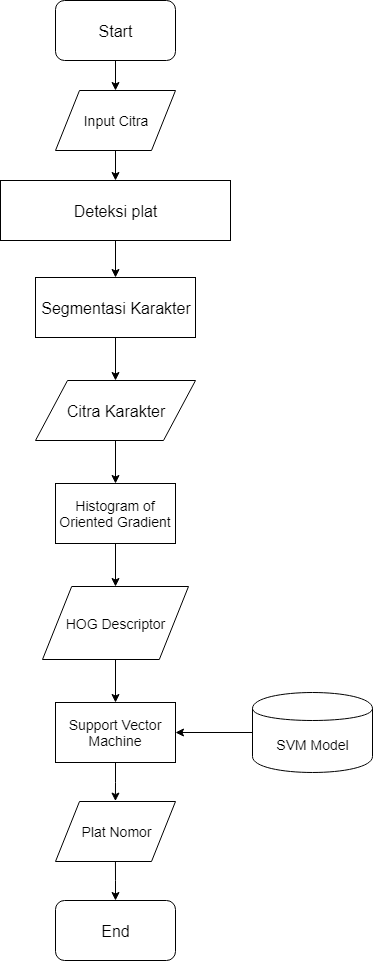
\includegraphics[width=7cm]{images/FlowchartTesting.png}}
%		\captionof{figure}{\textit{Flowchart Testing} Sistem Deteksi dan Pengenalan Plat Nomor\\}
%		\label{fig:FlowchartTesting}
%	\end{minipage}
%\end{adjustbox}
\noindent Kemudian untuk proses \textit{testing}, seperti terlihat pada Gambar \ref{fig:FlowchartGlobal}, terdapat beberapa proses yang sama seperti pada proses \textit{training}. Berikut ini adalah uraian dari \textit{flowchart} bagian kanan pada Gambar \ref{fig:FlowchartGlobal} yang dilakukan dalam penelitian ini:
\begin{enumerate}
	\item Citra pengujian yang digunakan didapatkan dari \textit{dataset} plat nomor kendaraan Universitas Telkom yang bernama \textit{Tel-U Vehicle Data-set V1.0}, penggunaan dari dataset ini sesuai dengan perizinan dari institusi yang bersangkutan. 
	\item Citra kendaraan akan melalui tahapan deteksi area plat kendaraan untuk mendapatkan citra plat.
	\item Citra plat yang didapatkan kemudian disegmentasi untuk mendapatkan citra karakter. 
	\item Citra yang akan menjadi masukan dari \textit{HOG} adalah citra hasil dari segmentasi karakter pada citra plat kendaraan hasil deteksi lokasi plat nomor kendaraan.
	\item Ukuran dari sel dan blok yang digunakan untuk proses ekstraksi fitur dengan menggunakan \textit{HOG} akan beragam sesuai dengan pengujian yang akan dilakukan.
	\item Pada tahap \textit{testing} model SVM yang digunakan berasal dari hasil keluaran model SVM pada tahap \textit{training}.
	\item Hasil keluaran akan berupa sebuah \textit{string} yang menunjukkan kumpulan karakter yang berhasil dikenali oleh sistem.\\
\end{enumerate}

\section{Analisis Manual}
\noindent Pada bagian ini dilakukan analisis tahapan proses pendeteksian dan pengenalan plat nomor dimulai dari tahapan mempersiapkan \textit{dataset}, mendeteksi lokasi plat nomor, melakukan segmentasi karakter, melakukan ekstraksi fitur dengan \textit{Histogram of Oriented Gradient}, dan melakukan proses latih dengan menggunakan \textit{Support Vector Machine}.
\subsection{\textit{Dataset}}
\noindent Citra plat kendaraan yang digunakan sebagai dataset adalah citra plat yang di-\textit{crop} secara manual seperti terlihat pada Gambar \ref{fig:ContohCitraPlat}.

\begin{adjustbox}{width=1\textwidth}
	\noindent
	\begin{minipage}{\linewidth}
		\framebox[\textwidth]{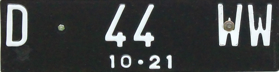
\includegraphics[width=8cm]{images/ContohPlat.PNG}}
		\captionof{figure}{Contoh citra plat yang digunakan\\}
		\label{fig:ContohCitraPlat}
	\end{minipage}
\end{adjustbox}

\noindent Dari citra plat akan dilakukan tahapan \textit{preprocessing}. Hasil akhir dari tahapan-tahapan tersebut dapat dilihat pada Gambar \ref{fig:ContohCitraPlatHasilPreprocessing}.

\begin{adjustbox}{width=1\textwidth}
	\noindent\begin{minipage}{\linewidth}
		\framebox[\textwidth]{
\includegraphics[width=8cm]{images/ContohHasilPreprocessing.PNG}}
		\captionof{figure}{Contoh citra plat setelah proses \textit{preprocessing}\\}
		\label{fig:ContohCitraPlatHasilPreprocessing}
	\end{minipage}
\end{adjustbox}

\noindent Dari citra plat hasil \textit{preprocessing}, berikutnya dilakukan proses segmentasi terhadap citra plat. Segmentasi horizontal bertujuan untuk memisahkan area karakter plat nomor dengan karakter tanggal masa berlaku plat nomor. Sedangkan segmentasi vertikal bertujuan untuk mendapatkan karakter karakter. Hasilnya dapat dilihat pada Gambar \ref{fig:CitraPlatHasilSegmentasiHorizontal} dan Gambar \ref{fig:CitraPlatHasilSegmentasiVertikal}.

\begin{adjustbox}{width=1\textwidth}
	\noindent
	\begin{minipage}{\linewidth}
		\framebox[\textwidth]{
\includegraphics[width=8cm]{images/HasilSegmentasiHorizontal.PNG}}
		\captionof{figure}{Citra plat setelah proses segmentasi horizontal\\}
		\label{fig:CitraPlatHasilSegmentasiHorizontal}
	\end{minipage}
\end{adjustbox}

\begin{adjustbox}{width=1\textwidth}
	\noindent\begin{minipage}{\linewidth}
		\framebox[\textwidth]{
\includegraphics[width=14cm]{images/HasilSegmentasiVertikal.PNG}}
		\captionof{figure}{Citra plat setelah proses segmentasi vertikal\\}
		\label{fig:CitraPlatHasilSegmentasiVertikal}
	\end{minipage}
\end{adjustbox}

\noindent Setelah didapatkan karakter-karakter dari plat nomor tersebut, berikutnya dilakukan proses \textit{scaling} dari ukuran seperti pada Gambar \ref{fig:CitraPlatHasilSegmentasiVertikal} menjadi ukuran 32 $\times$ 32 piksel. Alasan digunakannya ukuran 32 $\times$ 32 piksel adalah agar ukuran fitur dari \textit{HOG Descriptor} yang dihasilkan tidak terlalu besar. Hasil dari proses \textit{scaling} citra karakter dapat dilihat pada Gambar \ref{fig:ContohCitraDatasetPakai}. Citra karakter hasil proses \textit{scaling} itulah yang akan digunakan sebagai data latih.

\noindent Citra sampling memuat karakter terdiri dari angka 0 sampai dengan 9 dan karakter huruf kapital dari A sampai dengan Z. Untuk setiap karakter akan digunakan citra latih sebanyak tiga sampai dengan enam citra, hal ini untuk mengakomodasi beragam kondisi citra karakter sesuai dengan kondisi citra karakter pada plat mobil. Perbedaan dari karakter yang sama bisa disebabkan karena kondisi pencahayaan ketika pengambilan citra, modifikasi pada plat kendaraan misalnya menggunakan \textit{casing} pada dudukan plat, dan posisi kamera ketika pengambilan citra. Terlihat contoh citra karakter yang ditunjukkan pada Gambar \ref{fig:ContohCitraDatasetPakai} merupakan contoh karakter angka dan huruf kapital yang akan dipakai.

\begin{adjustbox}{width=1\textwidth}
	\noindent\begin{minipage}{\linewidth}
		\framebox[\textwidth]{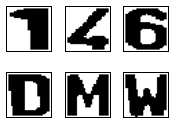
\includegraphics[width=8cm]{images/CitraDatasetPakai.PNG}}
		\captionof{figure}{Contoh citra karakter yang digunakan untuk tahap \textit{training}\\}
		\label{fig:ContohCitraDatasetPakai}
	\end{minipage}
\end{adjustbox}
\\

\subsection{Tahap Pendeteksian Lokasi Plat Nomor}
\noindent Skema alur dari tahap pendeteksian lokasi plat nomor adalah:

\begin{adjustbox}{width=1\textwidth}
	\noindent
	\begin{minipage}{\linewidth}
		\framebox[\textwidth]{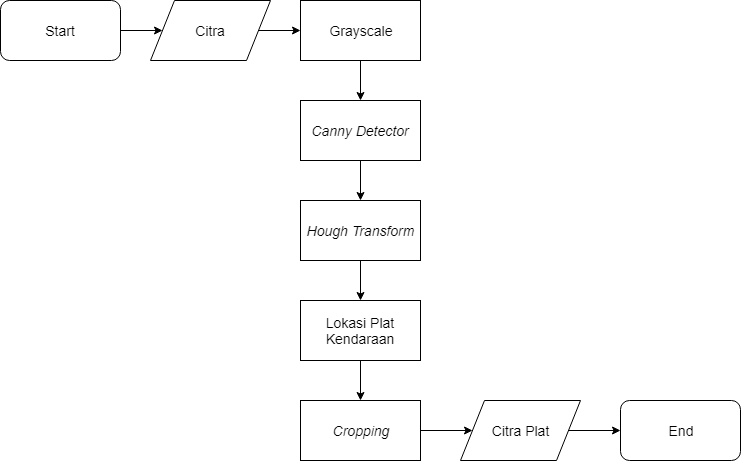
\includegraphics[width=13cm]{images/FlowchartDeteksiPlat.png}}
		\captionof{figure}{Skema Alur Pendeteksian Plat\\}
		\label{fig:SkemaAlurPendeteksianPlat}
	\end{minipage}
\end{adjustbox}\\

\subsubsection{\textit{Grayscale}}
\noindent Proses pertama adalah mengubah citra masukan dari citra RGB menjadi citra \textit{grayscale}, tujuan dari \textit{grayscaling} citra adalah untuk menghilangkan informasi warna dari setiap piksel citra. Untuk menghitung nilai derajat keabuan setiap piksel, diperoleh dengan menggunakan persamaan \ref{eq:grayscale}.
\noindent Di bawah merupakan contoh matriks citra asli dengan 3 \textit{channel} warna yaitu \textit{Red}, \textit{Green}, dan \textit{Blue} berukuran 5 $\times$ 5 piksel. 

\begin{adjustbox}{width=1\textwidth}
	\noindent\begin{minipage}{\linewidth}
		\framebox[\textwidth]{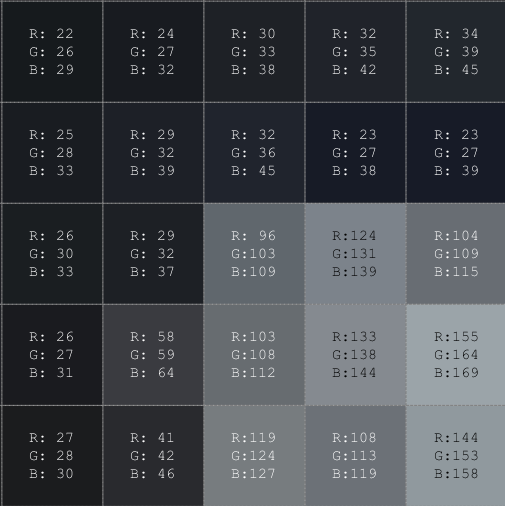
\includegraphics[width=8cm]{images/CitraMatriksAsal.PNG}}
		\captionof{figure}{Matriks Citra Asal berukuran 5 $\times$ 5\\}
		\label{fig:MatriksCitraAsal}
	\end{minipage}
\end{adjustbox} 

\noindent Dengan menggunakan persamaan \ref{eq:grayscale}, maka nilai matriks citra \textit{grayscale} pada titik (4,4) akan menjadi sebagai berikut:
\begin{table}[H]
	\begin{adjustbox}{width=1\textwidth}
		\begin{tabular}{|p{13.55cm}|}
			\hline
			\begin{equation}\nonumber
			\begin{aligned}
			Matriks[4,4] &= (0.299 * 133) + (0.587 * 138) + (0.114 * 144) \\
						 &= 137.189 \approx 137 
			\end{aligned}
			\end{equation}\\
			\hline
		\end{tabular}
	\end{adjustbox}
\end{table}
\noindent Perhitungan di atas dilakukan terhadap seluruh nilai matriks citra asal dan hasilnya adalah matriks citra berukuran 5 $\times$ 5 dengan satu nilai derajat keabuan.

\begin{adjustbox}{width=1\textwidth}
	\noindent\begin{minipage}{\linewidth}
		\framebox[\textwidth]{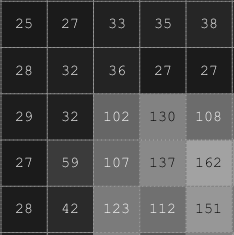
\includegraphics[width=6cm]{images/CitraMatriksGrayscale.PNG}}
		\captionof{figure}{Matriks Citra Hasil \textit{Grayscale}\\}
		\label{fig:MatriksCitraGrayscale}
	\end{minipage}
\end{adjustbox} \\

\subsubsection{Deteksi Tepi Canny}
\noindent Proses deteksi tepi dilakukan terhadap citra hasil \textit{grayscaling}. Pada penelitian ini, metode \textit{Canny Edge Detection} digunakan untuk mendapatkan tepian. Berikut adalah algoritme dari metode \textit{Canny Edge Detection} untuk mendapatkan tepian.
\begin{enumerate}[leftmargin=16pt]
	\item Citra masukan adalah citra dari hasil \textit{grayscaling} pada tahapan sebelumnya.
	\item Citra masukan diperhalus dengan menggunakan \textit{Gaussian Filter} untuk membuang derau.
	\item Lakukan operasi perhitungan gradien menggunakan operator Sobel untuk mendapatkan tepian yang tebal.
	\item Untuk menipiskan tepian yang didapat dari operasi sebelumnya maka teknik \textit{Non-Maxima Suppression} dilakukan dengan mencari nilai maksimum pada tepian.
	\item Buat 2 nilai \textit{threshold} yaitu \textit{high threshold} dan \textit{low threshold} untuk menentukan piksel mana yang masuk dalam kategori tepian kuat, tepian lemah, dan bukan tepian. Jika nilai dari piksel tersebut di atas \textit{high threshold}, maka piksel tersebut masuk ke dalam kategori tepian kuat, apabila nilai piksel berada di antara batas \textit{high threshold} dan \textit{low threshold}, maka piksel tersebut masuk ke dalam kategori tepian lemah, selebihnya akan masuk ke dalam kategori bukan tepian.
	\item Tahapan terakhir adalah \textit{Edge Linking} untuk menghubungkan tepian lemah dengan tepian kuat. Apabila piksel tepian lemah memiliki tetangga piksel (terhubung), maka piksel tersebut akan menjadi tepian.
	\item Citra keluaran adalah citra biner yang merupakan hasil pendeteksian tepi.
	
	\begin{adjustbox}{width=1\textwidth}
		\noindent
		\begin{minipage}{\linewidth}
			\framebox[\textwidth]{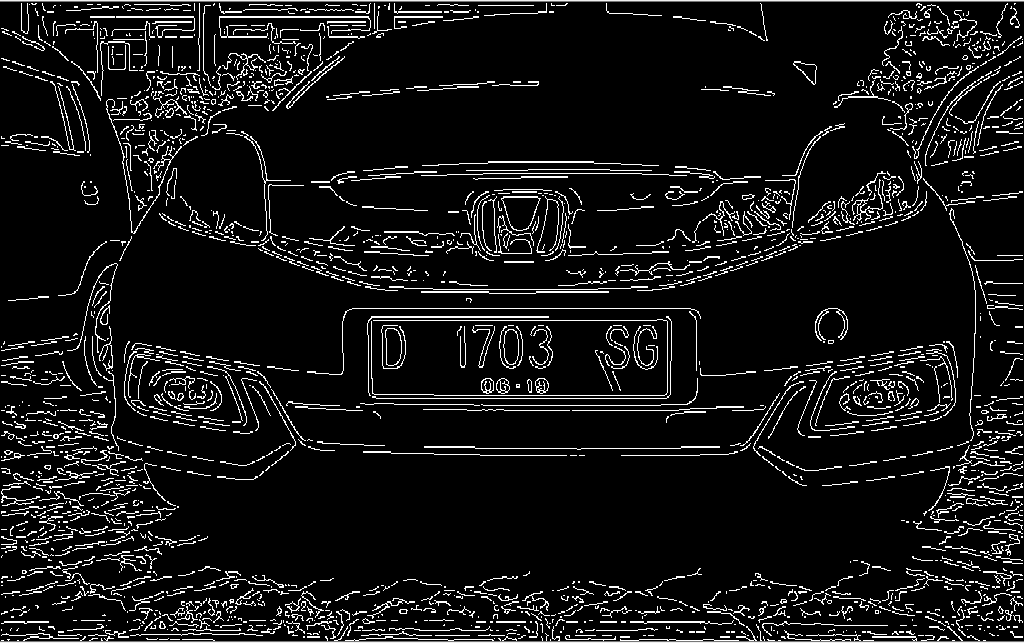
\includegraphics[width=13cm]{images/HasilCanny.png}}
			\captionof{figure}{Contoh Citra hasil deteksi tepi \textit{Canny}\\}
			\label{fig:HasilDeteksiTepi}
		\end{minipage}
	\end{adjustbox}\\
\end{enumerate}

\subsubsection{\textit{Hough Transform}}
\noindent Metode \textit{Hough Transform} yang digunakan adalah untuk identifikasi garis lurus. Dalam ekstraksi fitur \textit{Hough Transform} perlu menspesifikasikan \textit{accumulator space} untuk menyimpan nilai \textit{voting}. Untuk tahapan \textit{Hough Transform} ini akan menggunakan \textit{library} dari \textit{OpenCV} yaitu dengan menggunakan \textit{function} \textit{Imgproc.HoughLines()}. \textit{Function} \textit{Imgproc.HoughLines()} ini memiliki parameter masukan berupa citra biner hasil dari metode \textit{Canny Edge Detection}, \textit{range} sudut yang akan digunakan sebagai $\theta$ untuk membatasi sudut yang akan dicari, dan  nilai rho yang merupakan panjang garis dalam piksel. Spesifikasi \textit{accumulator space} ditentukan berdasarkan ukuran citra masukan. Berikut adalah algoritme dari metode \textit{Hough Transform} untuk mendapatkan garis lurus:
\begin{enumerate}
	\item Citra masukan adalah citra biner hasil deteksi tepi pada tahapan sebelumnya.
	\item Matriks \textit{Accumulator Space} didefinisikan sebagai \textit{array} 2 dimensi dengan sumbu horizontal menunjukkan nilai sudut ($\theta$) yang digunakan dan sumbu vertikal adalah nilai-nilai dari $\rho$.
	
	\begin{adjustbox}{width=1\textwidth}
		\noindent
		\begin{minipage}{\linewidth}
			\centering\framebox[8cm]{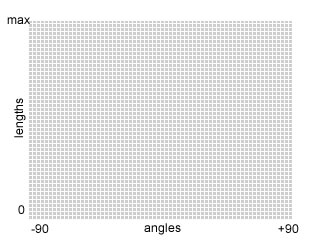
\includegraphics[width=8cm]{images/accumulatorspace.jpg}}
			\captionof{figure}{Ilustrasi matriks \textit{Accumulator Space}\\}
			\label{fig:MatriksAccumulatorSpace}
		\end{minipage}
	\end{adjustbox}
	\item Untuk setiap nilai piksel dari citra biner hasil deteksi tepian, apabila nilai piksel tersebut adalah 0, piksel tersebut diabaikan. Jika nilai piksel tersebut tidak 0, maka lakukan perhitungan nilai $\rho$ untuk piksel tersebut dengan menggunakan persamaan \ref{eq:PersamaanRho} dan lakukan \textit{voting} terhadap setiap nilai $\theta$ yang digunakan dengan menambahkan nilai pada matriks akumulator dengan koordinat ($\theta$, $\rho$) sebesar satu.
	\item Hasil dari perhitungan \textit{voting} akan dicari hasil-hasil \textit{voting} tertinggi untuk dijadikan kandidat garis melalui tahapan pencarian \textit{Hough Peaks}. Tahapan ini dilakukan dengan menentukan nilai \textit{threshold}, \textit{neighbourhood}, dan jumlah \textit{peaks} yang akan diambil.
	\item Hasil pencarian \textit{Hough Peaks} akan menghasilkan kumpulan nilai $\rho$ dan $\theta$, nilai ini kemudian diubah menjadi koordinat titik.
	\item Keluaran dari tahapan ini adalah \textit{array} yang berisi pasangan koordinat titik dari kandidat-kandidat garis yang didapat.\\
\end{enumerate}

\subsubsection{Tahap Validasi Plat Kendaraan}
\noindent Tahap selanjutnya setelah mendapatkan kandidat-kandidat garis adalah menyeleksi area plat nomor. Hal ini dilakukan melalui serangkaian tahapan sebagai berikut:
\begin{enumerate}
	\item Dari keseluruhan kandidat garis yang didapat, pisahkan kandidat garis vertikal dengan kandidat garis horizontal.
	\item Dari kandidat-kandidat garis vertikal akan ada yang menjadi batas kiri dan batas kanan dari area plat kendaraan. Setiap kandidat garis vertikal akan dipasangkan dengan garis vertikal lain dengan cara membandingkan mana garis yang lebih kanan. Hasilnya akan disimpan dalam \textit{array} yang berisi koordinat x dari masing-masing pasangan garis.
	\item Hitung lebar citra yang dibatasi dengan pasangan garis vertikal yang didapatkan, apabila lebar citra sesuai batasan ukuran yang ditentukan, maka pasangan garis tersebut akan menjadi kandidat dari batas kiri dan batas kanan dari plat nomor.
	\item Untuk setiap kandidat batas kiri dan batas kanan plat nomor, pasangkan dengan kandidat garis horizontal dan hitung tinggi citra yang dibatasi dengan batas horizontal, apabila tinggi citra sesuai dengan batasan ukuran yang ditentukan, maka pasangan garis tersebut akan menjadi batas atas dan batas bawah dari citra plat kendaraan.
	\item Jika masih terdapat lebih dari satu kandidat, maka pilih kandidat dengan rasio panjang : lebar yang paling mendekati rasio plat nomor kendaraan Indonesia, yaitu 1 : 3.
	\item Hasil dari tahapan ini adalah 4 titik koordinat yang merupakan koordinat citra plat. Citra plat akan diambil dari citra asal dengan menggunakan titik-titik koordinat tersebut.
\end{enumerate}

\begin{adjustbox}{width=1\textwidth}
	\noindent\begin{minipage}{\linewidth}
		\centering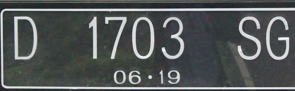
\includegraphics[width=8cm]{images/HasilPlat.png}
		\captionof{figure}{Contoh hasil citra plat\\}
		\label{fig:OutputPlat}
	\end{minipage}
\end{adjustbox}\\

\subsection{Tahapan Segmentasi Karakter}
\noindent Setelah mendapatkan kandidat plat, maka berikutnya dilakukan segmentasi karakter untuk mendapatkan citra-citra karakter yang terdapat pada plat nomor kendaraan. Pada tahapan segmentasi karakter, akan dilakukan dua tahapan, yaitu segmentasi vertikal untuk mendapatkan batas atas dan batas bawah daerah karakter, dan segmentasi horizontal untuk mendapatkan batas kiri dan batas kanan untuk setiap karakter. Untuk tahapan segmentasi karakter ini akan menggunakan \textit{method} dari \textit{library JavaOCR} seperti yang disebutkan pada \ref{tbl:FunctionJavaOCR}, yaitu \textit{LineExtractor.slice()} dan \textit{CharacterExtractor.slice()}. \textit{LineExtractor.slice()} digunakan untuk melakukan segmentasi horizontal, parameter dari \textit{method} tersebut adalah berkas citra plat yang sudah melalui tahapan \textit{preprocessing} dan berkas citra yang akan menampung hasil segmentasi horizontal. Sedangkan \textit{CharacterExtractor.slice()} digunakan untuk melakukan segmentasi vertikal dengan parameter citra hasil segmentasi horizontal, berkas citra yang akan menampung hasil segmentasi vertikal, dan dua parameter berikutnya adalah ukuran lebar dan tinggi citra untuk hasil proses \textit{scaling}. Berikut adalah langkah-langkah dari proses segmentasi karakter:
\begin{enumerate}
\item Citra masukan adalah citra plat hasil tahapan deteksi plat kendaraan yang sudah dilakukan \textit{preprocessing} menjadi citra biner.
\item Lakukan segmentasi vertikal untuk mendapatkan batas atas dan batas bawah dari area kandidat karakter.
\item Lakukan segmentasi horizontal untuk mendapatkan batas kiri dan batas kanan dari setiap citra karakter.
\item Setiap citra karakter yang didapatkan akan di-\textit{scaling} menjadi ukuran 32 $\times$ 32 piksel. Hal ini bertujuan untuk menjaga konsistensi ukuran citra karakter yang digunakan untuk proses \textit{training} dan proses \textit{testing}. Hasil dari segmentasi seperti yang ditunjukkan pada Gambar \ref{fig:OutputSegmentasi} ditambahkan satu piksel lebih untuk setiap batas kiri, kanan, atas, dan bawah dari citra, tujuannya adalah agar bentuk karakter yang didapatkan ketika proses ekstraksi fitur dengan menggunakan metode \textit{Histogram of Oriented Gradient} menjadi lebih baik.
\item Keluaran dari tahapan ini adalah citra karakter yang terdapat pada plat nomor.
\end{enumerate}

\noindent Pada penelitian ini, tahapan segmentasi karakter akan menggunakan \textit{library} dari Java OCR dan \textit{method} atau \textit{function} yang digunakan dapat dilihat pada tabel \ref{tbl:FunctionJavaOCR}.\\
\\
\begin{adjustbox}{width=1\textwidth}
	\noindent\begin{minipage}{\linewidth}
		\centering
\includegraphics[width=14cm]{images/OutputSegmentasi.png}
		\captionof{figure}{Contoh hasil keluaran dari tahapan segmentasi\\}
		\label{fig:OutputSegmentasi}
	\end{minipage}
\end{adjustbox}\\

\subsection{\textit{Histogram of Oriented Gradient}}
\noindent Pada proses \textit{Histogram of Oriented Gradients}, masukan untuk proses ini berupa citra yang berasal dari hasil segmentasi. Perhitungan fitur dari metode \textit{Histogram of Oriented Gradient} ini dilakukan per citra karakter hasil segmentasi. Keluaran dari proses ini adalah matriks fitur vektor dari hasil perhitungan \textit{Histogram of Oriented Gradients}. Berikut merupakan langkah-langkah untuk menghitung matriks fitur vektor. Pada Gambar \ref{fig:MatriksCitraHasilPreprocessing} dapat dilihat hasil dari proses \textit{resize} dan \textit{crop} citra \textit{grayscale} berukuran 8 $\times$ 4 piksel.

\begin{table}[H]
	\centering
	\begin{small}
		\begin{tabular}{|p{2cm}|p{2cm}|p{2cm}|p{2cm}|}
			\hline
			89 & 92 & 88 & 92 \\
			\hline
			90 & 88 & 90 & 86 \\
			\hline
			91 & 90 & 90 & 94 \\
			\hline
			91 & 122 & 91 & 122 \\
			\hline
			89 & 90 & 89 & 91 \\
			\hline
			90 & 85 & 90 & 86 \\
			\hline
			91 & 90 & 92 & 93 \\
			\hline
			91 & 122 & 91 & 120 \\
			\hline
		\end{tabular}
	\end{small}
	\captionof{figure}{Matriks citra hasil \textit{preprocessing}\\}
	\label{fig:MatriksCitraHasilPreprocessing}
\end{table}

\begin{enumerate}
\item Proses pertama adalah untuk menghitung nilai gradien dari posisi vertikal dan horizontal untuk setiap piksel menggunakan persamaan \ref{eq:PersamaanGradienX} dan \ref{eq:PersamaanGradienY}. Contoh perhitungannya untuk piksel koordinat (2,5) dan hasil dari tahap ini dapat dilihat pada Gambar \ref{fig:MatriksCitraHasilGradienX} dan \ref{fig:MatriksCitraHasilGradienY}:
\begin{equation*}
	G_{x}(2,5) = 89 - 89 = 0
\end{equation*}
\begin{equation*}
	G_{y}(2,5) = 85 - 122 = -37
\end{equation*}
\begin{table}[H]
	\centering
	\begin{small}
		\begin{tabular}{|p{2cm}|p{2cm}|p{2cm}|p{2cm}|}
			\hline
			92 & -1 & 0 & -88 \\
			\hline
			88 & 0 & -2 & -90 \\
			\hline
			90 & -1 & 4 & -90 \\
			\hline
			122 & 0 & 0 & -91 \\
			\hline
			90 & 0 & 1 & -89 \\
			\hline
			85 & 0 & 1 & -90 \\
			\hline
			90 & 1 & 3 & -92 \\
			\hline
			122 & 0 & -2 & -91 \\
			\hline
		\end{tabular}
	\end{small}
	\captionof{figure}{Matriks hasil Perhitungan Gradien sumbu X\\}
	\label{fig:MatriksCitraHasilGradienX}
\end{table}
\begin{table}[H]
	\centering
	\begin{small}
		\begin{tabular}{|p{2cm}|p{2cm}|p{2cm}|p{2cm}|}
			\hline
			90 & 88 & 90 & 86 \\
			\hline
			2 & -2 & 2 & 2 \\
			\hline
			1 & 34 & 1 & 36 \\
			\hline
			-2 & 0 & -1 & -3 \\
			\hline
			-1 & -37 & -1 & -36 \\
			\hline
			2 & 0 & 3 & 2 \\
			\hline
			1 & 37 & 1 & 34 \\
			\hline
			-91 & -90 & -92 & -93 \\
			\hline
		\end{tabular}
	\end{small}
	\captionof{figure}{Matriks hasil Perhitungan Gradien sumbu Y\\}
	\label{fig:MatriksCitraHasilGradienY}
\end{table}
\item Untuk setiap piksel, hitung \textit{magnitude} gradien dan arah gradien menggunakan persamaaan \ref{eq:PersamaanMagnitude} dan \ref{eq:PersamaanArah}. Contoh perhitungannya untuk piksel koordinat (2,5) dan hasil dari tahap ini dapat dilihat pada Gambar \ref{fig:MatriksHasilMagnitude}:
\begin{equation*}
M(2,5) = \sqrt{0^2 + (-37)^2} = 37
\end{equation*}
\begin{equation*}
\theta(2,5) = arctan\frac{-37}{0} \approx 90
\end{equation*}
\begin{table}[H]
	\centering
	\begin{small}
		\begin{tabular}{|p{2cm}|p{2cm}|p{2cm}|p{2cm}|}
			\hline
			128.70 & 88.01 & 90 & 123.05 \\
			\hline
			88.03 & 2 & 2.83 & 90.02 \\
			\hline
			90.01 & 34.02 & 4.12 & 96.93 \\
			\hline
			122.02 & 0 & 1 & 91.05 \\
			\hline
			90.01 & 37 & 1.41 & 96.01 \\
			\hline
			85.02 & 0 & 3.16 & 90.02 \\
			\hline
			90.01 & 37.01 & 3.16 & 98.08 \\
			\hline
			152.2 & 90 & 92.02 & 130.12 \\
			\hline
		\end{tabular}
	\end{small}
	\captionof{figure}{Matriks hasil Perhitungan \textit{Magnitude}\\}
	\label{fig:MatriksHasilMagnitude}
\end{table}
\begin{table}[H]
	\centering
	\begin{small}
		\begin{tabular}{|p{2cm}|p{2cm}|p{2cm}|p{2cm}|}
			\hline
			44.37 & 90.65 & 89.99 & 135.66 \\
			\hline
			1.30 & 90.03 & 135 & 178.73 \\
			\hline
			0.64 & 91.69 & 14.04 & 158.19 \\
			\hline
			179.06 & 0 & 90.06 & 1.89 \\
			\hline
			179.36 & 90 & 135 & 22.02 \\
			\hline
			1.35 & 0 & 71.57 & 178.73 \\
			\hline
			0.64 & 88.45 & 18.44 & 159.72 \\
			\hline
			143.28 & 90 & 88.76 & 45.62 \\
			\hline
		\end{tabular}
	\end{small}
	\captionof{figure}{Matriks hasil Perhitungan Arah\\}
	\label{fig:MatriksHasilPerhitunganArah}
\end{table}
\item Kemudian, tentukan ukuran sel, ukuran blok dan jumlah \textit{oriented histogram bins}. Pada penelitian Dalas dan Triggs untuk mendeteksi pejalan kaki sebelumnya, didapat bahwa ukuran sel sebesar 8 $\times$ 8 piksel, ukuran blok sebesar 2 $\times$ 2 ukuran sel dan jumlah bin sebanyak 9 sudah dapat menghasilkan akurasi yang dapat mendeteksi pejalan kaki dengan cukup baik dibandingkan dengan ukuran-ukuran lainnya. Untuk contoh perhitungan analisis kali ini jumlah \textit{oriented histogram bins} yang dipakai sebanyak 4 buah, sehingga didapat nilai sudut setiap \textit{histogram bin} yaitu 180 / 4 = 45. Untuk ukuran sel dipilih sebesar 2 $\times$ 2 piksel dan ukuran blok sebesar 2 $\times$ 2 sel. Untuk setiap blok, terdapat \textit{overlapping} sebesar 50\% dari ukuran blok. Dengan demikian akan didapatkan perhitungan sebagai berikut:
\begin{enumerate}[label=\alph*.]
\item Jumlah sel adalah 8, terdiri dari 4 sel vertikal dan 2 sel horizontal.
\item Jumlah blok adalah 3, terdiri dari 3 blok vertikal dan 1 blok horizontal.
\end{enumerate}
\item Kemudian untuk setiap sel, tentukan perhitungan \textit{Histogram of Oriented Gradient} dengan melakukan \textit{voting} dari arah gradien dan \textit{magnitude} gradien, dimana arah gradien akan menjadi sudut \textit{bin}, dan \textit{magnitude} gradien akan menjadi bobot nilai. Berikut merupakan contoh proses \textit{voting} untuk piksel dengan koordinat (2,5).
\begin{equation*}
M(2,5) = 37
\end{equation*}
\begin{equation*}
\theta(2,5) = 90
\end{equation*}
Sehingga untuk \textit{bin} dengan sudut 90 akan mendapat nilai bobot sebesar 37 yang didapatkan dari nilai gradien \textit{magnitude}-nya.
Lakukan proses tersebut untuk setiap sel sehingga masing-masing sel akan mempunyai \textit{Histogram of Oriented Gradient}. Berikut contoh hasil perhitungan metode \textit{Histogram of Oriented Gradient} pada sel yang terdapat koordinat piksel (2,5) dapat dilihat pada Gambar \ref{fig:HasilHOG}.\\
\begin{adjustbox}{width=1\textwidth}
	\noindent\begin{minipage}{\linewidth}
		\framebox[\textwidth]{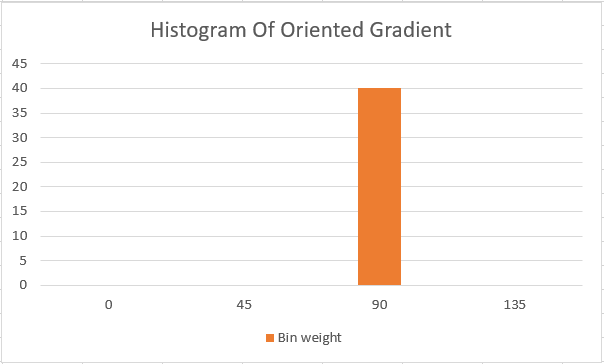
\includegraphics[width=12cm]{images/HistogramOfOrientedGradient.PNG}}
		\captionof{figure}{Contoh hasil \textit{Histogram of Oriented Gradient} untuk sel yang memiliki piksel dengan koordinat (2,5)}
		\label{fig:HasilHOG}
	\end{minipage}
\end{adjustbox}
\item Kemudian untuk setiap blok, akan dilakukan normalisasi dengan menggabungkan hasil histogram dari setiap sel dalam bloknya. Adapun proses normalisasi dapat menggunakan 4 algoritme yaitu, \textit{L1-Norm}, \textit{L1-Sqrt}, \textit{L2-Norm}, dan \textit{L2-Hys}. Pada penelitian ini, penulis menggunakan algoritme normalisasi \textit{L2-Norm} karena berdasarkan penelitian sebelumnya, hasil yang didapat lebih baik dari algoritme lainnya. Persamaan algoritme untuk proses normalisasi menggunakan \textit{L2-Norm} didapat dengan menggunakan persamaan \ref{eq:L2-Norm}. Di bawah adalah contoh perhitungan normalisasi untuk blok pertama:
\begin{table}[H]
	\centering
	\begin{small}
		\begin{tabular}{|p{1cm}|p{1cm}|p{1cm}|p{1cm}|p{1cm}|p{1cm}|p{1cm}|p{1cm}|}
			\hline
			87.28 & 129.45 & 88.73 & 1.28 & 89.28 & 0 & 89.99 & 126.62 \\
			\hline
			208.2 & 1.27 & 32.74 & 3.82 & 140.04 & 5.11 & 0.99 & 46.96 \\
			\hline
			171.21 & 2.55 & 36.99 & 1.28 & 136.49 & 48.28 & 1.87 & 3.96 \\
			\hline
			116.74 & 2.55 & 125.74 & 124.19 & 55.74 & 132.16 & 91.28 & 44.21 \\
			\hline
		\end{tabular}
	\end{small}
	\captionof{figure}{Matriks hasil Perhitungan Histogram untuk seluruh sel\\}
	\label{fig:MatriksHasilPerhitunganHistogram}
\end{table}
Berdasarkan matriks pada Gambar \ref{fig:MatriksHasilPerhitunganHistogram}. Elemen matriks yang akan kita gunakan dalam perhitungan normalisasi ini adalah seluruh elemen baris pertama dan baris kedua.
\begin{equation*}
L2_{Norm} = \sqrt{87.28^2 + 129.45^2 + \ldots + 0.99^2 + 46.96^2} = 361.428
\end{equation*}
Kemudian untuk setiap nilai dari histogram dari sel dalam blok tersebut akan dibagi dengan nilai hasil normalisasinya. Di bawah adalah contoh hasil normalisasi histogram dari sel pertama (matriks hasil perhitungan histogram baris pertama kolom 1-4):
\begin{gather*}
\begin{bmatrix}
0.24148 & 0.35815 & 0.2455 & 0.00353 \\
\end{bmatrix}
\end{gather*}
Lakukan proses normalisasi untuk setiap blok dengan menggeser secara horizontal sejauh 1 kali ukuran sel dan secara vertikal sejauh 1 kali ukuran sel sampai blok tersebut sudah berada di bawah kanan dari citra. Kemudian hasil dari proses normalisasi akan disusun menjadi matriks besar dengan jumlah kolom sebesar  \textit{jumlah bin} $\times$ \textit{lebar blok dalam satuan sel} $\times$ \textit{jumlah pergeseran horizontal} dan jumlah baris sebesar \textit{jumlah pergeseran vertikal} $\times$ \textit{tinggi blok dalam satuan sel} , dengan perhitungan tersebut, dalam analisis saat ini didapatkan ukuran matriks sebesar 6 $\times$ 8. Dalam analisis ini, hasil keluaran dari metode \textit{Histogram of Oriented Gradient} ada sebanyak 48 fitur. Di bawah adalah hasil fitur vektor untuk metode \textit{Histogram of Oriented Gradient} setelah melewati proses normalisasi.\\
\begin{table}[H]
	\centering
	\begin{small}
		\begin{tabular}{|p{1cm}|p{1cm}|p{1cm}|p{1cm}|p{1cm}|p{1cm}|p{1cm}|p{1cm}|}
			\hline
			0.24 & 0.36 & 0.25 & 0.00 & 0.25 & 0.00 & 0.25 & 0.35 \\ \hline
			0.58 & 0.00 & 0.09 & 0.01 & 0.39 & 0.01 & 0.00 & 0.13 \\ \hline
			0.61 & 0.00 & 0.10 & 0.01 & 0.41 & 0.01 & 0.00 & 0.14 \\ \hline
			0.50 & 0.01 & 0.11 & 0.00 & 0.40 & 0.14 & 0.01 & 0.01 \\ \hline
			0.48 & 0.01 & 0.10 & 0.00 & 0.38 & 0.14 & 0.01 & 0.01 \\ \hline
			0.33 & 0.01 & 0.35 & 0.35 & 0.16 & 0.37 & 0.26 & 0.12 \\ \hline
		\end{tabular}
	\end{small}
	\captionof{figure}{Matriks hasil Normalisasi\\}
	\label{fig:MatriksHasilNormalisasi}
\end{table}
Setelah mendapatkan matriks \textit{HOG descriptor} di atas. Langkah berikutnya adalah menjadikan matriks tersebut sebagai vektor. Hal ini dilakukan dengan mengambil setiap baris dari matriks dan memasukkannya ke dalam matriks vektor berukuran 1 $\times$ jumlah fitur. Vektor inilah yang akan dijadikan sebagai masukan bagi metode \textit{Machine Learning} yang akan digunakan dalam penelitian ini.\\
\end{enumerate}

\subsection{\textit{Support Vector Machine}}
\noindent Tahapan terakhir dari sistem deteksi dan pengenalan plat nomor kendaraan adalah klasifikasi karakter. Masukan untuk proses ini berupa fitur \textit{HOG Descriptor} untuk setiap citra karakter plat nomor. Tahapan ini bertujuan untuk mengklasifikasikan fitur-fitur dari \textit{HOG descriptor} yang dihasilkan dari perhitungan metode \textit{Histogram of Oriented Gradient} agar dapat dikenali sebagai karakter. \textit{Support Vector Machine} yang akan digunakan dalam penelitian menggunakan \textit{library} dari Weka SVM. Untuk \textit{function} atau \textit{method} yang digunakan pada \textit{library} tersebut dapat dilihat pada tabel \ref{tbl:FunctionWeka}. \textit{Support Vector Machine} termasuk dalam algoritme \textit{supervised learning}. Konsep dasar dari metode ini adalah untuk menemukan sebuah \textit{separating hyperplane} (bidang) yang dapat memisahkan dua kelas sebagai keputusan klasifikasi. Dalam penelitian ini karakter yang akan dikenali adalah huruf A sampai dengan Z dan angka dari 0 sampai dengan 9 sehingga akan terdapat 36 kelas untuk proses klasifikasi.
%\noindent Tabel \ref{tbl:filteredDataset} merupakan rincian jumlah citra pada masing-masing \textit{dataset} setelah dilakukan pemilihan.
%\begin{table}[H]
%	\centering
%	\begin{small}
%		\captionof{table}{Rincian \textit{Dataset} yang telah dipilih\label{tbl:filteredDataset}}
%		\begin{tabular}{|p{4cm}|p{1cm}|p{3cm}|p{3cm}|}
%			\hline
%			\textbf{Nama \textit{Dataset}} &\textbf{Folder} & \textbf{Jumlah Citra} & \textbf{Jumlah Posisi Manusia}\\
%			\hline
%			\textit{Clothing Store} 			& - & 770 & 1631 \\
%			\hline
%			\multirow{3}{*}\textit{Outdoor}	& 31 & 46 & 218 \\\cline{2-4}
%			& 54 & 84 & 371 \\\cline{2-4}
%			& 56 & 113 & 496 \\\hline
%		\end{tabular}
%	\end{small}
%\end{table}



\newpage
	\setcounter{page}{1}
	\setlength\LTleft{0pt}            % default: \fill
	\setlength\LTright{0pt}           % default: \fill	
	%-----------------------------------------------------------------------------%
\chapter{IMPLEMENTASI DAN PENGUJIAN}
%-----------------------------------------------------------------------------%

%
\vspace{4.5pt}
\noindent Pada bab ini akan menjelaskan mengenai proses implementasi dan pengujian terhadap sistem yang telah dibangun berdasarkan penjelasan pada bab sebelumnya.\\

\section{Lingkungan Implementasi}
\noindent Pada lingkungan implementasi, akan dijelaskan mengenai perangkat yang digunakan dalam proses pembangunan sistem baik dari perangkat keras maupun perangkat lunak yang digunakan.\\

\subsection{Spesifikasi Perangkat Keras}
\noindent Spesifikasi dari perangkat keras yang digunakan dalam pembangunan aplikasi adalah sebagai berikut:
\begin{enumerate}
\item \textit{Laptop} ASUS A442UQ
\item \textit{Processor} Intel Core i7-7500U CPU @ 2.7GHz
\item \textit{Hard Disk} kapasitas 1TB
\item RAM 16GB\\
\end{enumerate}

\subsection{Lingkungan Perangkat Lunak}
\noindent Spesifikasi dari perangkat lunak yang digunakan dalam pembangunan aplikasi adalah sebagai berikut:
\begin{enumerate}
\item Sistem Operasi Windows 10 Home 64 bit.
\item Netbeans IDE 8.2
\item Java Development Kit (JDK) 1.8.0{\_}161
\item \textit{Library} OpenCV 3.4.6\\
\end{enumerate}

%\subsection{Penjelasan \textit{Dataset}}
%\noindent Pada implementasi digunakan dua buah \textit{dataset} yaitu \textit{Clothing Store} dan \textit{Outdoor}. Seperti yang telah dijelaskan pada bab 2, 80\% citra dari \textit{dataset Clothing Store} akan digunakan untuk pembelajaran dan 20\% citra lainya untuk pengujian. Sementara \textit{dataset Outdoor} yang terdiri atas 3 buah folder yaitu 31, 54, dan 56, di mana seluruh citra pada folder 56 untuk data belajar, lalu folder 31 dan folder 54 untuk data uji. Pada masing-masing \textit{dataset} didapatkan masing-masing citra positif yaitu berisi manusia sesuai dengan berkas \textit{ground truth} sedangkan citra negatif yaitu berisi selain manusia didapatkan secara acak yang tidak berpotongan dengan daerah citra manusia. Ukuran dari citra negatif adalah 65 $\times$ 80 piksel. Rincian dari jumlah citra, citra positif, dan citra negatif dapat dilihat pada tabel \ref{tbl:rincianDataset}.
%\begingroup
%\setlength{\LTleft}{-20cm plus -1fill}
%\setlength{\LTright}{\LTleft}
%\begin{small}
%\begin{longtable}{|c|c|c|c|c|c|c|}
%\caption{Rincian \textit{Dataset} untuk Implementasi}
%\label{tbl:rincianDataset}
%\endhead
%\hline
%\textit{\textbf{Dataset}}			& \textbf{Folder}			& \textbf{Keterangan}	& \textbf{Citra Belajar}	& \textbf{Citra Uji}	& \multicolumn{2}{c|}{\textbf{Total}} \\ \hline
%\multirow{3}{*}{\textit{Clothing Store}}	& \multirow{3}{*}{-}		& Citra				& 616					& 154				& \multicolumn{2}{c|}{770}            \\ \cline{3-7} 
%								&						& Manusia			& 1160					& 471				& 1631     & \multirow{2}{*}{5092}    \\ \cline{3-6}
%								&						& Lain-lain			& 2766					& 695				& 3461     &                          \\ \hline
%\multirow{9}{*}{\textit{Outdoor}}		& \multirow{3}{*}{31}	& Citra				& - 						& 46				& \multicolumn{2}{c|}{46}             \\ \cline{3-7} 
%								&						& Manusia			& - 						& 218				& 218      & \multirow{2}{*}{427}     \\ \cline{3-6}
%								&						& Lain-lain			& - 						& 209				& 209      &                          \\ \cline{2-7} 
%								& \multirow{3}{*}{54}	& Citra				& - 						& 84				& \multicolumn{2}{c|}{84}             \\ \cline{3-7} 
%								&						& Manusia			& - 						& 371				& 371      & \multirow{2}{*}{744}     \\ \cline{3-6}
%								&						& Lain-lain			& - 						& 373				& 373      &                          \\ \cline{2-7} 
%								& \multirow{3}{*}{56}	& Citra				& 113					& - 					& \multicolumn{2}{c|}{113}            \\ \cline{3-7} 
%								&						& Manusia			& 496					& - 					& 496      & \multirow{2}{*}{999}     \\ \cline{3-6}
%								&						& Lain-lain			& 503					& - 					& 503      &                          \\ \hline
%\end{longtable}
%\end{small}
%\endgroup

\section{Implementasi Perangkat Lunak}
\noindent Pada bab ini akan dijelaskan mengenai implementasi aplikasi untuk pengenalan karakter pada citra plat kendaraan. Di bawah ini merupakan daftar \textit{class} dan \textit{method} beserta penjelasan mengenai cara kerja program.\\
\subsection{Daftar \textit{Class} dan \textit{Method} Gradient}
\noindent Berikut adalah tabel berisi \textit{method} pada \textit{class} Gradient. \textit{Class} Gradient digunakan untuk menyimpan nilai \textit{orientation} dan nilai \textit{magnitude} dari suatu piksel citra.
\begin{small}
	\begin{longtable}{| p {0.5cm} | p {4.5cm} | p {4cm} | p {1.5cm} | p {3cm} |}
		\caption{Daftar \textit{Method Class Gradient} } \\
		\hline
		\textbf{No}  & \textbf{Nama \textit{method}}  & \textbf{Masukan}  & \textbf{Keluaran} & \textbf{Keterangan} \\
		\hline
		\endfirsthead
		\endhead	
		1	& Gradient & double orientation, double magnitude & void & Metode \textit{constructor} yang digunakan untuk inisialisasi objek dari kelas Gradient dengan nilai \textit{orientation} dan \textit{magnitude} yang didapatkan dari perhitungan. \\
		\hline
		2	& getOrientation() & & double & Metode untuk mengembalikan nilai \textit{orientation} dari suatu piksel.\\
		\hline
		3	& getMagnitude() & & double & Metode yang digunakan untuk mengembalikan nilai \textit{magnitude} dari suatu piksel.\\
		\hline
		4	& setOrientation() & double orientation & void & Metode untuk mengatur nilai \textit{orientation} dari objek Gradient berdasarkan nilai \textit{orientation} yang dijadikan masukkan.\\
		\hline
		5	& setMagnitude() & double magnitude & void & Metode yang digunakan untuk mengatur nilai \textit{magnitude} dari objek Gradient berdasarkan nilai \textit{magnitude}  yang dijadikan masukkan.\\
		\hline
	\end{longtable}
\end{small}

\subsection{Daftar \textit{Class} dan \textit{Method} GradientCell}
\noindent Berikut adalah tabel berisi \textit{method} pada \textit{class} GradientCell. \textit{Class} GradientCell digunakan untuk menyimpan nilai gradien dari setiap sel.
\begin{small}
	\begin{longtable}{| p {0.5cm} | p {4.5cm} | p {3cm} | p {2.5cm} | p {3cm} |}
		\caption{Daftar \textit{Method Class GradientCell} } \\
		\hline
		\textbf{No}  & \textbf{Nama \textit{method}}  & \textbf{Masukan}  & \textbf{Keluaran} & \textbf{Keterangan} \\
		\hline
		\endfirsthead
		\endhead	
		1	& GradientCell() & int length & void & Metode \textit{constructor} yang digunakan untuk inisialisasi objek dari kelas GradientCell. \\
		\hline
		2	& getGradients() & & List \textless Gradient \textgreater & Metode untuk mengembalikan \textit{List} dari gradien-gradien yang terdapat .\\
		\hline
	\end{longtable}
\end{small}

\subsection{Daftar \textit{Class} dan \textit{Method} HOG}
\noindent Berikut adalah tabel berisi \textit{method} pada \textit{class} HOG. \textit{Class} HOG digunakan untuk proses ekstraksi fitur dari citra karakter.
\begin{small}
	\begin{longtable}{| p {0.5cm} | p {4.5cm} | p {4cm} | p {1.5cm} | p {3cm} |}
		\caption{Daftar \textit{Method Class HOG} } \\
		\hline
		\textbf{No}  & \textbf{Nama \textit{method}}  & \textbf{Masukan}  & \textbf{Keluaran} & \textbf{Keterangan} \\
		\hline
		\endfirsthead
		\endhead	
		1	& HOG() & Integer[][] image, int cellHeight, int cellWidth, int blockSize, int numBins & void & Metode \textit{constructor} yang digunakan untuk inisialisasi objek dari kelas HOG. \\
		\hline
		2	& extractHOGFeatures() & & double[] & Metode untuk mengekstraksi fitur \textit{HOG descriptor} dari citra.\\
		\hline
		3	& calculateGradientAndCells() & & void & Metode yang digunakan untuk menghitung nilai gradien, \textit{magnitude}, dan orientasi untuk setiap sel.\\
		\hline
		4	& createHistograms() & 	& void & Metode untuk membentuk histogram untuk mencatat persebaran arah dari setiap sel.\\
		\hline
		5	& histogramNormalization() & & void & Melakukan normalisasi \textit{L2-Norm} untuk setiap elemen pada histogram.\\
		\hline
		6	& createDescriptor() & & void & Membentuk \textit{HOG descriptor} dari hasil normalisasi histogram.\\
		\hline
	\end{longtable}
\end{small}

\subsection{Daftar \textit{Class} dan \textit{Method} SVM}
\noindent Berikut adalah tabel berisi \textit{method} pada \textit{class} SVM. \textit{Class} SVM digunakan untuk perhitungan klasifikasi.
\begin{small}
	\begin{longtable}{| p {0.5cm} | p {4cm} | p {3cm} | p {3cm} | p {3cm} |}
		\caption{Daftar \textit{Method Class SVM} } \\
		\hline
		\textbf{No}  & \textbf{Nama \textit{method}}  & \textbf{Masukan}  & \textbf{Keluaran} & \textbf{Keterangan} \\
		\hline
		\endfirsthead
		\endhead	
		1	& calculateRBFKernel() & double[][] data, double sigma,
		int classSource, int classTarget	& double &	Menghitung nilai RBF Kernel.\\
		\hline
		2	& createRBFMatrix() & double[][] data, double[] sigma & double[][] & Membentuk matriks RBF dari data fitur.\\
		\hline
		3	& createLinearEquation() & double[][] rbfMatrix, double[] classList	& double[][]	& Membuat persamaan linear dari matriks RBF.\\
		\hline
		4	& getSolutions() & double[][] linearEquationMatix, double[] classList	& Matrix & Mendapatkan solusi dari persamaan linear yaitu nilai alpha dan bias.\\
		\hline
		5	& createRBFTestMatrix() & double[][] data, double sigma, double[] classList	& double & Membentuk matriks RBF untuk data pengujian.\\
		\hline
		6	& classify() & double[][] solutions, double[] rbfTest, double[] classList	& double & Mendapatkan nilai hasil klasifikasi berdasarkan data uji dan nilai alpha dan bias.\\
		\hline
		7	& getDataFromText() & String path	& double[][] & Membaca matriks fitur dari file teks.\\
		\hline
		
	\end{longtable}
\end{small}
%Package cnn
%\subsubsection{Daftar \textit{Class} dan \textit{Method}}
%\noindent \textit{Class} CNN merupakan kelas yang berfungsi untuk melaksanakan proses \textit{Convolutional Neural Network} dengan arsitektur lapisan dan \textit{hyperparameter} yang telah ditentukan, lihat tabel \ref{tbl:classCNN}.
%\begingroup
%\setlength{\LTleft}{-20cm plus -1fill}
%\setlength{\LTright}{\LTleft}
%\begin{small}
%\begin{longtable}{|p{0.4cm}|p{2cm}|p{1.8cm}|p{1.8cm}|p{1.7cm}|p{3.55cm}|}
%	\caption{Daftar \textit{Method} pada \textit{Class} CNN \label{tbl:classCNN}}\\
%	\hline
%	\multirow{2}{*}{\textbf{No}} & \multirow{2}{*}{\textit{\textbf{Method}}} & \multicolumn{2}{c|}{\textit{\textbf{Input}}} & \multirow{2}{*}{\textit{\textbf{Output}}} & 
%	\multirow{2}{*}{\textbf{Keterangan}}\\
%	\cline{3-4}
%	& & \textbf{Tipe} & \textbf{Variabel} & & \\
%	\endfirsthead
%	\multicolumn{6}{c}{\textbf{\tablename~\thetable} Daftar \textit{Method} pada \textit{Class} CNN (Lanjutan)} \\ \hline
%	\multirow{2}{*}{\textbf{No}} & \multirow{2}{*}{\textit{\textbf{Method}}} & \multicolumn{2}{c|}{\textit{\textbf{Input}}} & \multirow{2}{*}{\textit{\textbf{Output}}} & 
%	\multirow{2}{*}{\textbf{Keterangan}}\\
%	\cline{3-4}
%	& & \textbf{Tipe} & \textbf{Variabel} & & \\
%	\endhead
%	\hline
%	1 & CNN & List$<$\newline Layer$>$,\newline double,\newline double,\newline int,\newline String & layers,\newline alpha,\newline alphaDivider,\newline saveModel,\newline pathModel & - & Konstruktor yang menerima dan menyimpan nilai \textit{hyperparameter} serta melakukan inisialisasi nilai pada kelas CNN.\\
%	\hline
%	2 & train & List$<$\newline TrainImage\newline$>$,\newline int & trainImg,\newline epoch & - & Melakukan tahap pembelajaran dari citra dengan pengulangan sebanyak \textit{epoch} serta menyimpan hasil pembelajaran.\\
%	\hline
%	3 & train & TrainImage & trainImg & - & Melakukan tahap pembelajaran untuk 1 citra, tahap \textit{forward} dan \textit{backward} yang mencakup menghitung turunan atau gradien lalu memperbarui nilai parameter berdasarkan gradien masing-masing.\\
%	\hline
%	4 & forward & TrainImage,\newline Process & img,\newline process & - & Melakukan tahap \textit{forward} pada setiap lapisan dan menghitung hasil berdasarkan proses pelatihan atau pengujian.\\
%	\hline
%	5 &  setGradient & TrainImage & img & - & Melakukan perhitungan gradien pada setiap lapisan.\\
%	\hline
%	6 & getData & - & - & List$<Data>$ & Menambahkan seluruh data yang telah dihitung pada setiap lapisan pada sebuah kelas \textit{List}.\\
%	\hline
%	7 & updateParams & - & - & - & Memperbarui parameter bobot berdasarkan data yang telah didapatkan dalam bentuk \textit{List}.\\
%	\hline
%	8 & update & int,\newline double,\newline double[] & j,\newline gradient,\newline weight & - & Menambahkan nilai bobot sesuai dengan gradiennya.\\
%	\hline
%	9 & test & List$<$\newline TrainImage\newline $>$ & trainImg & double & Melakukan tahap \textit{forward} untuk setiap gambar dan mengembalikan nilai akurasi.\\
%	\hline
%	10 & isHuman & double[][],\newline double & img,\newline threshold & boolean & Menguji adanya citra manusia yang dibatasi dengan probabilitas hasil pengujian.\\
%	\hline
%\end{longtable}
%\end{small}
%\endgroup

%\subsubsection{\textit{Class} CNNLoader}
%\noindent \textit{Class} CNNLoader merupakan kelas yang berfungsi untuk melakukan penyimpanan serta pemuatan model hasil pembelajaran \textit{Convolutional Neural Network}, lihat tabel \ref{tbl:classCNNLoader}.
%\begingroup
%\setlength{\LTleft}{-20cm plus -1fill}
%\setlength{\LTright}{\LTleft}
%\begin{small}
%\begin{longtable}{|p{0.4cm}|p{2cm}|p{1.8cm}|p{1.8cm}|p{1.7cm}|p{3.55cm}|}
%	\caption{Daftar \textit{Method} pada \textit{Class} CNNLoader \label{tbl:classCNNLoader}}\\
%	\hline
%	\multirow{2}{*}{\textbf{No}} & \multirow{2}{*}{\textit{\textbf{Method}}} & \multicolumn{2}{c|}{\textit{\textbf{Input}}} & \multirow{2}{*}{\textit{\textbf{Output}}} & 
%	\multirow{2}{*}{\textbf{Keterangan}}\\
%	\cline{3-4}
%	& & \textbf{Tipe} & \textbf{Variabel} & & \\
%	\endfirsthead
%	\multicolumn{6}{c}{\textbf{\tablename~\thetable} Daftar \textit{Method} pada \textit{Class} CNNLoader (Lanjutan)} \\
%	\hline
%	\multirow{2}{*}{\textbf{No}} & \multirow{2}{*}{\textit{\textbf{Method}}} & \multicolumn{2}{c|}{\textit{\textbf{Input}}} & \multirow{2}{*}{\textit{\textbf{Output}}} & 
%	\multirow{2}{*}{\textbf{Keterangan}}\\
%	\cline{3-4}
%	& & \textbf{Tipe} & \textbf{Variabel} & & \\
%	\endhead
%	\hline
%	1 & saveModel & String,\newline CNN & fileName,\newline cnn & - & Menyimpan model \textit{Convolutional Neural Network} dengan nama yang telah ditentukan.\\
%	\hline
%	2 & loadModel & String & fileName & CNN & Memuat model \textit{Convolutional Neural Network} yang telah disimpan sebelumnya.\\
%	\hline
%\end{longtable}
%\end{small}
%\endgroup

%Package cnn.layer
%\subsubsection{\textit{Class} Data}
%\noindent \textit{Class} Data merupakan kelas yang berfungsi untuk menyimpan data yang digunakan pada tahap \textit{Convolutional Neural Network}, lihat tabel \ref{tbl:classData}.
%\begingroup
%\setlength{\LTleft}{-20cm plus -1fill}
%\setlength{\LTright}{\LTleft}
%\begin{small}
%\begin{longtable}{|p{0.4cm}|p{2cm}|p{1.8cm}|p{1.8cm}|p{1.7cm}|p{3.55cm}|}
%	\caption{Daftar \textit{Method} pada \textit{Class} Data \label{tbl:classData}}\\
%	\hline
%	\multirow{2}{*}{\textbf{No}} & \multirow{2}{*}{\textit{\textbf{Method}}} & \multicolumn{2}{c|}{\textit{\textbf{Input}}} & \multirow{2}{*}{\textit{\textbf{Output}}} & 
%	\multirow{2}{*}{\textbf{Keterangan}}\\
%	\cline{3-4}
%	& & \textbf{Tipe} & \textbf{Variabel} & & \\
%	\endfirsthead
%	\multicolumn{6}{c}{\textbf{\tablename~\thetable} Daftar \textit{Method} pada \textit{Class} Data (Lanjutan)} \\
%	\hline
%	\multirow{2}{*}{\textbf{No}} & \multirow{2}{*}{\textit{\textbf{Method}}} & \multicolumn{2}{c|}{\textit{\textbf{Input}}} & \multirow{2}{*}{\textit{\textbf{Output}}} & 
%	\multirow{2}{*}{\textbf{Keterangan}}\\
%	\cline{3-4}
%	& & \textbf{Tipe} & \textbf{Variabel} & & \\
%	\endhead
%	\hline
%	1 & Data & Size & size & - & Konstruktor yang menerima dan menyimpan besar ukuran.\\
%	\hline
%	2 & addImage-\newline Data & double[][] & trainImg & - & Menyimpan nilai dari citra.\\
%	\hline
%	3 & getSize & - & - & Size & Digunakan untuk mendapatkan ukuran dari data.\\
%	\hline
%	4 & getWeight & int & index & double & Digunakan untuk mendapatkan bobot pada indeks 1 dimensi.\\
%	\hline
%	5 & getWeight & int,\newline int,\newline int & x,\newline y,\newline depth & double & Digunakan untuk mendapatkan bobot pada indeks 3 dimensi.\\
%	\hline
%	6 & setWeight & double & value & - & Digunakan untuk mendapatkan bobot pada indeks 1 dimensi.\\
%	\hline
%	7 & setWeight & int,\newline int,\newline int,\newline double & x,\newline y,\newline depth,\newline value & - & Digunakan untuk menetapkan nilai bobot pada indeks 3 dimensi.\\
%	\hline
%	8 & addWeight & int,\newline int,\newline int,\newline double & x,\newline y,\newline depth,\newline value & - & Digunakan untuk menambahkan nilai bobot.\\
%	\hline
%	9 & getGradient & int,\newline int,\newline int & x,\newline y,\newline depth & double & Digunakan untuk mendapatkan ukuran dari data pada indeks 3 dimensi.\\
%	\hline
%	10 & getGradient & int & index & double & Digunakan untuk mendapatkan ukuran dari data pada indeks 1 dimensi\\
%	\hline
%	11 & setGradient & int,\newline int,\newline int,\newline double & x,\newline y,\newline depth,\newline value & - & Digunakan untuk menentukan nilai gradien pada indeks 3 dimensi.\\
%	\hline
%	12 & setGradient & int & value & - & Digunakan untuk menentukan nilai gradien pada indeks 1 dimensi.\\
%	\hline
%	13 & addGradient & int,\newline int,\newline int,\newline double & x,\newline y,\newline depth,\newline value & - & Digunakan untuk nambahkan nilai gradien dengan indeks 3 dimensi.\\
%	\hline
%	14 & addGradient & int,\newline double & index,\newline value & - & Digunakan untuk nambahkan nilai gradien pada indeks 1 dimensi.\\
%	\hline
%	15 & calculate-\newline Index & int,\newline int,\newline int & x,\newline y,\newline depth & int & Digunakan untuk mendapatkan indeks pada 1 dimensi.\\
%	\hline
%	16 & clearGradient & - & - & - & Digunakan untuk hapus seluruh gradien.\\
%	\hline
%	17 & getWeights & - & - & double[] & Digunakan untuk mendapatkan seluruh bobot.\\
%	\hline
%	18 & getGradients & - & - & double[] & Digunakan untuk mendapatkan seluruh gradien.\\
%	\hline
%\end{longtable}
%\end{small}
%\endgroup

%\subsubsection{\textit{Class} Size}
%\noindent \textit{Class} Size merupakan kelas yang berfungsi untuk menyimpan informasi ukuran lebar, tinggi, dan kedalaman. Penjelasan mengenai kelas ini dapat dilihat pada tabel \ref{tbl:classSize}.
%\begingroup
%\setlength{\LTleft}{-20cm plus -1fill}
%\setlength{\LTright}{\LTleft}
%\begin{small}
%\begin{longtable}{|p{0.4cm}|p{2cm}|p{1.8cm}|p{1.8cm}|p{1.7cm}|p{3.55cm}|}
%	\caption{Daftar \textit{Method} pada \textit{Class} Size \label{tbl:classSize}}\\
%	\hline
%	\multirow{2}{*}{\textbf{No}} & \multirow{2}{*}{\textit{\textbf{Method}}} & \multicolumn{2}{c|}{\textit{\textbf{Input}}} & \multirow{2}{*}{\textit{\textbf{Output}}} & 
%	\multirow{2}{*}{\textbf{Keterangan}}\\
%	\cline{3-4}
%	& & \textbf{Tipe} & \textbf{Variabel} & & \\
%	\endfirsthead
%	\multicolumn{6}{c}{\textbf{\tablename~\thetable} Daftar \textit{Method} pada \textit{Class} Size (Lanjutan)} \\
%	\hline
%	\multirow{2}{*}{\textbf{No}} & \multirow{2}{*}{\textit{\textbf{Method}}} & \multicolumn{2}{c|}{\textit{\textbf{Input}}} & \multirow{2}{*}{\textit{\textbf{Output}}} & 
%	\multirow{2}{*}{\textbf{Keterangan}}\\
%	\cline{3-4}
%	& & \textbf{Tipe} & \textbf{Variabel} & & \\
%	\endhead
%	\hline
%	1 & Size & - & - & - & Konstruktor kosong ketika objek dibuat tanpa parameter.\\
%	\hline
%	2 & Size & int,\newline int,\newline int & width,\newline height,\newline depth & - & Konstruktor yang menerima dan menerima informasi ukuran.\\
%	\hline
%	3 & getWidth & - & - & int & Digunakan untuk mendapatkan lebar citra.\\
%	\hline
%	2 & setWidth & int & width & - & Digunakan untuk menentukan lebar citra.\\
%	\hline
%	2 & getHeight & - & - & int & Digunakan untuk mendapatkan tinggi citra.\\
%	\hline
%	2 & setHeight & int & height & - & Digunakan untuk menentukan tinggi citra.\\
%	\hline
%	2 & getDepth & - & - & int & Digunakan untuk mendapatkan kedalaman citra.\\
%	\hline
%	2 & setDepth & int & depth & - & Digunakan untuk menentukan kedalaman citra.\\
%	\hline
%	2 & toString & - & - & String & Mengembalikan informasi ukuran dalam bentuk text.\\
%	\hline
%\end{longtable}
%\end{small}
%\endgroup

%Package cnn.layer
%\subsubsection{\textit{Class} Layer}
%\noindent \textit{Class} Layer merupakan sebuah kelas abstrak untuk lapisan pada \textit{Convolutional Neural Network}. Penjelasan mengenai kelas ini dapat dilihat pada tabel \ref{tbl:classLayer}.
%\begingroup
%\setlength{\LTleft}{-20cm plus -1fill}
%\setlength{\LTright}{\LTleft}
%\begin{small}
%\begin{longtable}{|p{0.4cm}|p{2cm}|p{1.8cm}|p{1.8cm}|p{1.7cm}|p{3.55cm}|}
%	\caption{Daftar \textit{Method} pada \textit{Class} Layer \label{tbl:classLayer}}\\
%	\hline
%	\multirow{2}{*}{\textbf{No}} & \multirow{2}{*}{\textit{\textbf{Method}}} & \multicolumn{2}{c|}{\textit{\textbf{Input}}} & \multirow{2}{*}{\textit{\textbf{Output}}} & 
%	\multirow{2}{*}{\textbf{Keterangan}}\\
%	\cline{3-4}
%	& & \textbf{Tipe} & \textbf{Variabel} & & \\
%	\endfirsthead
%	\multicolumn{6}{c}{\textbf{\tablename~\thetable} Daftar \textit{Method} pada \textit{Class} Layer (Lanjutan)} \\
%	\hline
%	\multirow{2}{*}{\textbf{No}} & \multirow{2}{*}{\textit{\textbf{Method}}} & \multicolumn{2}{c|}{\textit{\textbf{Input}}} & \multirow{2}{*}{\textit{\textbf{Output}}} & 
%	\multirow{2}{*}{\textbf{Keterangan}}\\
%	\cline{3-4}
%	& & \textbf{Tipe} & \textbf{Variabel} & & \\
%	\endhead
%	\hline
%	1 & forward & Data & inData & Data & Menerima data masukan untuk diproses dan menghasilkan data keluaran.\\
%	\hline
%	2 & setGradient & - & - & - & Menghitung dan menentukan nilai gradien.\\
%	\hline
%	3 & getData & - & - & List$<$Data$>$ & Digunakan untuk mendapatkan seluruh data dalam bentuk \textit{List}.\\
%	\hline
%	4 & getType & - & - & LayerType & Digunakan untuk mendapatkan keterangan jenis lapisan.\\
%	\hline
%	5 & setType & LayerType & type & - & Digunakan untuk menentukan jenis dari lapisan.\\
%	\hline
%	6 & getMapSize & - & - & Size & Digunakan untuk mendapatkan informasi ukuran.\\
%	\hline
%	7 & setMapSize & Size & mapSize & - & Digunakan untuk menentukan ukuran.\\
%	\hline
%	8 & setInData & Data & data & - & Digunakan untuk menentukan data masukan.\\
%	\hline
%	9 & getOutData & - & - & Data & Digunakan untuk mendapatkan data keluaran.\\
%	\hline
%	10 & setData & Data & data & - & Digunakan untuk menentukan data keluaran.\\
%	\hline
%\end{longtable}
%\end{small}
%\endgroup

%\subsubsection{\textit{Class} InputLayer}
%\noindent \textit{Class} InputLayer merupakan kelas untuk menyimpan informasi pada lapisan masukan dan di-\textit{extends} dengan \textit{class} Layer. Penjelasan kelas ini dapat dilihat pada tabel \ref{tbl:classInputLayer}.
%\begingroup
%\setlength{\LTleft}{-20cm plus -1fill}
%\setlength{\LTright}{\LTleft}
%\begin{small}
%\begin{longtable}{|p{0.4cm}|p{2cm}|p{1.8cm}|p{1.8cm}|p{1.7cm}|p{3.55cm}|}
%	\caption{Daftar \textit{Method} pada \textit{Class} InputLayer \label{tbl:classInputLayer}}\\
%	\hline
%	\multirow{2}{*}{\textbf{No}} & \multirow{2}{*}{\textit{\textbf{Method}}} & \multicolumn{2}{c|}{\textit{\textbf{Input}}} & \multirow{2}{*}{\textit{\textbf{Output}}} & 
%	\multirow{2}{*}{\textbf{Keterangan}}\\
%	\cline{3-4}
%	& & \textbf{Tipe} & \textbf{Variabel} & & \\
%	\endfirsthead
%	\multicolumn{6}{c}{\textbf{\tablename~\thetable} Daftar \textit{Method} pada \textit{Class} InputLayer (Lanjutan)} \\
%	\hline
%	\multirow{2}{*}{\textbf{No}} & \multirow{2}{*}{\textit{\textbf{Method}}} & \multicolumn{2}{c|}{\textit{\textbf{Input}}} & \multirow{2}{*}{\textit{\textbf{Output}}} & 
%	\multirow{2}{*}{\textbf{Keterangan}}\\
%	\cline{3-4}
%	& & \textbf{Tipe} & \textbf{Variabel} & & \\
%	\endhead
%	\hline
%	1 & InputLayer & Size & mapSize & - & Konstruktor untuk menerima parameter dan menentukan jenis layer.\\
%	\hline
%	2 & setTrain-\newline Image & TrainImage & trainImg & - & Digunakan untuk menentukan citra masukan yang akan diproses.\\
%	\hline
%	3 & getImgInput & - & - & double[][] & Digunakan untuk mendapatkan informasi mengenai citra masukan.\\
%	\hline
%	4 & getLabel & - & - & int & Digunakan untuk mendapatkan label dari citra masukan.\\
%	\hline
%	5 & forward & Data & data & Data & Untuk menerima data masukan dan menentukan data keluaran serta mengembalikan nilai keluaran tersebut.\\
%	\hline
%	6 & setGradient & - & - & - & Pada lapisan masukan tidak dilakukan perhitungan gradien.\\
%	\hline
%	7 & getData & - & - & List$<$Data$>$ & Mengembalikan list kosong karena tidak terdapat data yang perlu diperbarui.\\
%	\hline
%\end{longtable}
%\end{small}
%\endgroup

%\subsubsection{\textit{Class} ConvolutionLayer}
%\noindent \textit{Class} ConvolutionLayer merupakan kelas untuk proses konvolusi pada tahap \textit{forward} maupun \textit{backward} dan di-\textit{extends} dengan \textit{class} Layer. Penjelasan kelas ini dapat dilihat pada tabel \ref{tbl:classConvolutionLayer}.
%\begingroup
%\setlength{\LTleft}{-20cm plus -1fill}
%\setlength{\LTright}{\LTleft}
%\begin{small}
%\begin{longtable}{|p{0.4cm}|p{2cm}|p{1.8cm}|p{1.8cm}|p{1.7cm}|p{3.55cm}|}
%	\caption{Daftar \textit{Method} pada \textit{Class} ConvolutionLayer \label{tbl:classConvolutionLayer}}\\
%	\hline
%	\multirow{2}{*}{\textbf{No}} & \multirow{2}{*}{\textit{\textbf{Method}}} & \multicolumn{2}{c|}{\textit{\textbf{Input}}} & \multirow{2}{*}{\textit{\textbf{Output}}} & 
%	\multirow{2}{*}{\textbf{Keterangan}}\\
%	\cline{3-4}
%	& & \textbf{Tipe} & \textbf{Variabel} & & \\
%	\endfirsthead
%	\multicolumn{6}{c}{\textbf{\tablename~\thetable} Daftar \textit{Method} pada \textit{Class} ConvolutionLayer (Lanjutan)} \\
%	\hline
%	\multirow{2}{*}{\textbf{No}} & \multirow{2}{*}{\textit{\textbf{Method}}} & \multicolumn{2}{c|}{\textit{\textbf{Input}}} & \multirow{2}{*}{\textit{\textbf{Output}}} & 
%	\multirow{2}{*}{\textbf{Keterangan}}\\
%	\cline{3-4}
%	& & \textbf{Tipe} & \textbf{Variabel} & & \\
%	\endhead
%	\hline
%	1 & Convolution-\newline Layer & Size & kernelSize & - & Konstruktor yang menerima ukuran \textit{kernel} dan melakukan inisialisasi atribut.\\
%	\hline
%	2 & initOutData & Data & inData & Data & Melakukan inisialisasi ukuran untuk data keluaran.\\
%	\hline
%	3 & forward & Data & inData & Data & Melakukan proses perhitungan konvolusi data masukan dengan \textit{kernel} dan bias, lalu hasilnya disimpan dan dikembalikan sebagai data keluaran untuk diproses pada lapisan selanjutnya.\\
%	\hline
%	4 & setGradient & - & - & - & Menghitung gradien pada lapisan konvolusi dengan menggunakan gradien dari lapisan selanjutnya.\\
%	\hline
%	5 & getData & - & - & List$<$Data$>$ & Mengembalikan seluruh data \textit{kernel} dan bias yang digunakan pada lapisan konvolusi.\\
%	\hline
%\end{longtable}
%\end{small}
%\endgroup

%\subsubsection{\textit{Class} RELULayer}
%\noindent \textit{Class} RELU merupakan kelas yang di-\textit{extends} dengan \textit{class} Layer untuk menghitung hasil data masukan yang dimasukkan ke fungsi aktivasi \textit{rectified linear unit} (ReLU). Penjelasan kelas ini dapat dilihat pada tabel \ref{tbl:classRELULayer}.
%\begingroup
%\setlength{\LTleft}{-20cm plus -1fill}
%\setlength{\LTright}{\LTleft}
%\begin{small}
%\begin{longtable}{|p{0.4cm}|p{2cm}|p{1.8cm}|p{1.8cm}|p{1.7cm}|p{3.55cm}|}
%	\caption{Daftar \textit{Method} pada \textit{Class} RELULayer \label{tbl:classRELULayer}}\\
%	\hline
%	\multirow{2}{*}{\textbf{No}} & \multirow{2}{*}{\textit{\textbf{Method}}} & \multicolumn{2}{c|}{\textit{\textbf{Input}}} & \multirow{2}{*}{\textit{\textbf{Output}}} & 
%	\multirow{2}{*}{\textbf{Keterangan}}\\
%	\cline{3-4}
%	& & \textbf{Tipe} & \textbf{Variabel} & & \\
%	\endfirsthead
%	\multicolumn{6}{c}{\textbf{\tablename~\thetable} Daftar \textit{Method} pada \textit{Class} RELULayer (Lanjutan)} \\
%	\hline
%	\multirow{2}{*}{\textbf{No}} & \multirow{2}{*}{\textit{\textbf{Method}}} & \multicolumn{2}{c|}{\textit{\textbf{Input}}} & \multirow{2}{*}{\textit{\textbf{Output}}} & 
%	\multirow{2}{*}{\textbf{Keterangan}}\\
%	\cline{3-4}
%	& & \textbf{Tipe} & \textbf{Variabel} & & \\
%	\endhead
%	\hline
%	1 & reluActivation & double & value & double & Menghitung sebuah nilai untuk digunakan pada fungsi aktivasi ReLU.\\
%	\hline
%	2 & forward & Data & inData & Data & Menghitung seluruh nilai dari data masukan dengan fungsi aktivasi ReLU.\\
%	\hline
%	3 & setGradient & - & - & - & Menghitung gradien dengan turunan dari fungsi aktivasi ReLU.\\
%	\hline
%	4 & getData & - & - & List$<$Data$>$ & Mengembalikan list data kosong karena tidak terdapat data yang perlu diperbarui.\\
%	\hline
%\end{longtable}
%\end{small}
%\endgroup

%\subsubsection{\textit{Class} SubsamplingLayer}
%\noindent \textit{Class} SubsamplingLayer merupakan kelas untuk menyimpan hasil dari proses \textit{subsampling} atau \textit{pooling} dan di-\textit{extends} dengan \textit{class} Layer. Penjelasan kelas ini dapat dilihat pada tabel \ref{tbl:classSubsamplingLayer}.
%\begingroup
%\setlength{\LTleft}{-20cm plus -1fill}
%\setlength{\LTright}{\LTleft}
%\begin{small}
%\begin{longtable}{|p{0.4cm}|p{2cm}|p{1.8cm}|p{1.8cm}|p{1.7cm}|p{3.55cm}|}
%	\caption{Daftar \textit{Method} pada \textit{Class} SubsamplingLayer \label{tbl:classSubsamplingLayer}}\\
%	\hline
%	\multirow{2}{*}{\textbf{No}} & \multirow{2}{*}{\textit{\textbf{Method}}} & \multicolumn{2}{c|}{\textit{\textbf{Input}}} & \multirow{2}{*}{\textit{\textbf{Output}}} & 
%	\multirow{2}{*}{\textbf{Keterangan}}\\
%	\cline{3-4}
%	& & \textbf{Tipe} & \textbf{Variabel} & & \\
%	\endfirsthead
%	\multicolumn{6}{c}{\textbf{\tablename~\thetable} Daftar \textit{Method} pada \textit{Class} SubsamplingLayer (Lanjutan)} \\
%	\hline
%	\multirow{2}{*}{\textbf{No}} & \multirow{2}{*}{\textit{\textbf{Method}}} & \multicolumn{2}{c|}{\textit{\textbf{Input}}} & \multirow{2}{*}{\textit{\textbf{Output}}} & 
%	\multirow{2}{*}{\textbf{Keterangan}}\\
%	\cline{3-4}
%	& & \textbf{Tipe} & \textbf{Variabel} & & \\
%	\endhead
%	\hline
%	1 & Sub-\newline sampling-\newline Layer & Size & scaleSize & - & Konstruktor yang menerima ukuran untuk \textit{pooling}.\\
%	\hline
%	2 & initOutData & Data & inData & Data & Melakukan inisialisasi ukuran untuk data keluaran.\\
%	\hline
%	3 & initMaxData & Data & outData & Data & Melakukan inisialisasi ukuran untuk indeks dengan nilai tertinggi.\\
%	\hline
%	2 & forward & Data & inData & Data & Melakukan proses \textit{pooling} sesuai dengan ukuran yang telah ditentukan dan menyimpan indeks dari nilai yang tertinggi untuk digunakan saat tahap \textit{backward}.\\
%	\hline
%	3 & setGradient & - & - & - & Menentukan nilai gradien berdasarkan nilai tertinggi saat tahap \textit{forward} dan nilai lainnya adalah 0.\\
%	\hline
%	4 & getData & - & - & List$<$Data$>$ & Mengembalikan list data kosong karena tidak terdapat data yang perlu diperbarui.\\
%	\hline
%\end{longtable}
%\end{small}
%\endgroup

%\subsubsection{\textit{Class} FullyConnectedLayer}
%\noindent \textit{Class} FullyConnectedLayer merupakan kelas yang berfungsi untuk menerima seluruh data hasil dari lapisan sebelumnya dan selanjutnya dimasukkan ke fungsi. \textit{Class} ini juga di-\textit{extends} dengan \textit{class} Layer. Penjelasan kelas ini dapat dilihat pada tabel \ref{tbl:classFullyConnectedLayer}.
%\begingroup
%\setlength{\LTleft}{-20cm plus -1fill}
%\setlength{\LTright}{\LTleft}
%\begin{small}
%\begin{longtable}{|p{0.4cm}|p{2cm}|p{1.8cm}|p{1.8cm}|p{1.7cm}|p{3.55cm}|}
%	\caption{Daftar \textit{Method} pada \textit{Class} FullyConnectedLayer \label{tbl:classFullyConnectedLayer}}\\
%	\hline
%	\multirow{2}{*}{\textbf{No}} & \multirow{2}{*}{\textit{\textbf{Method}}} & \multicolumn{2}{c|}{\textit{\textbf{Input}}} & \multirow{2}{*}{\textit{\textbf{Output}}} & 
%	\multirow{2}{*}{\textbf{Keterangan}}\\
%	\cline{3-4}
%	& & \textbf{Tipe} & \textbf{Variabel} & & \\
%	\endfirsthead
%	\multicolumn{6}{c}{\textbf{\tablename~\thetable} Daftar \textit{Method} pada \textit{Class} FullyConnectedLayer (Lanjutan)} \\
%	\hline
%	\multirow{2}{*}{\textbf{No}} & \multirow{2}{*}{\textit{\textbf{Method}}} & \multicolumn{2}{c|}{\textit{\textbf{Input}}} & \multirow{2}{*}{\textit{\textbf{Output}}} & 
%	\multirow{2}{*}{\textbf{Keterangan}}\\
%	\cline{3-4}
%	& & \textbf{Tipe} & \textbf{Variabel} & & \\
%	\endhead
%	\hline
%	1 & Fully-\newline Connected-\newline Layer & Size & kernelSize & - & Konstruktor yang menerima ukuran \textit{kernel} dan inisialisasi atribut.\\
%	\hline
%	2 & forward & Data & inData & Data & Membentuk data masukan dalam bentuk 1 dimensi dan dikalikan dengan \textit{kernel} yang berukuran sama dengan masukan, kemudian dijumlahkan sebagai data keluaran.\\
%	\hline
%	3 & setGradient & - & - & - & Menghitung dan menentukan nilai gradien pada data masukan, \textit{kernel}, serta bias.\\
%	\hline
%	4 & getData & - & - & List$<$Data$>$ & Mengembalikan seluruh data \textit{kernel} dan bias yang digunakan pada lapisan ini.\\
%	\hline
%\end{longtable}
%\end{small}
%\endgroup

%\subsubsection{\textit{Class} SoftmaxLayer}
%\noindent \textit{Class} SoftmaxLayer merupakan kelas yang di-\textit{extends} dengan \textit{class} Layer untuk menghitung hasil data masukan yang dimasukkan ke fungsi \textit{softmax}. Penjelasan kelas ini dapat dilihat pada tabel \ref{tbl:classSoftmaxLayer}.
%\begingroup
%\setlength{\LTleft}{-20cm plus -1fill}
%\setlength{\LTright}{\LTleft}
%\begin{small}
%\begin{longtable}{|p{0.4cm}|p{2cm}|p{1.8cm}|p{1.8cm}|p{1.7cm}|p{3.55cm}|}
%	\caption{Daftar \textit{Method} pada \textit{Class} SoftmaxLayer \label{tbl:classSoftmaxLayer}}\\
%	\hline
%	\multirow{2}{*}{\textbf{No}} & \multirow{2}{*}{\textit{\textbf{Method}}} & \multicolumn{2}{c|}{\textit{\textbf{Input}}} & \multirow{2}{*}{\textit{\textbf{Output}}} & 
%	\multirow{2}{*}{\textbf{Keterangan}}\\
%	\cline{3-4}
%	& & \textbf{Tipe} & \textbf{Variabel} & & \\
%	\endfirsthead
%	\multicolumn{6}{c}{\textbf{\tablename~\thetable} Daftar \textit{Method} pada \textit{Class} SoftmaxLayer (Lanjutan)} \\
%	\hline
%	\multirow{2}{*}{\textbf{No}} & \multirow{2}{*}{\textit{\textbf{Method}}} & \multicolumn{2}{c|}{\textit{\textbf{Input}}} & \multirow{2}{*}{\textit{\textbf{Output}}} & 
%	\multirow{2}{*}{\textbf{Keterangan}}\\
%	\cline{3-4}
%	& & \textbf{Tipe} & \textbf{Variabel} & & \\
%	\endhead
%	\hline
%	1 & Softmax-\newline Layer & Size & size & - & Konstruktor yang menerima ukuran hasil akhir dari \textit{Convolutional Neural Network}.\\
%	\hline
%	2 & forward & Data & inData & Data & Melakukan perhitungan menggunakan fungsi \textit{softmax} yang telah dinormalisasi dengan nilai maksimal nilai masukan.\\
%	\hline
%	3 & setGradient & - & - & - & Menghitung nilai \textit{error} dari label sebenarnya.\\
%	\hline
%	4 & getData & - & - & List$<$Data$>$ & Mengembalikan list data kosong karena tidak terdapat data yang perlu diperbarui.\\
%	\hline
%\end{longtable}
%\end{small}
%\endgroup

%Package kalman
%\subsubsection{\textit{Class} Kalman}
%\noindent \textit{Class} Kalman merupakan kelas yang berfungsi untuk melakukan proses Kalman \textit{filtering} yang mencakup tahap prediksi dan pembaruan, lihat tabel \ref{tbl:classKalman}.
%\begingroup
%\setlength{\LTleft}{-20cm plus -1fill}
%\setlength{\LTright}{\LTleft}
%\begin{small}
%\begin{longtable}{|p{0.4cm}|p{2cm}|p{1.8cm}|p{1.8cm}|p{1.7cm}|p{3.55cm}|}
%	\caption{Daftar \textit{Method} pada \textit{Class} Kalman \label{tbl:classKalman}}\\
%	\hline
%	\multirow{2}{*}{\textbf{No}} & \multirow{2}{*}{\textit{\textbf{Method}}} & \multicolumn{2}{c|}{\textit{\textbf{Input}}} & \multirow{2}{*}{\textit{\textbf{Output}}} & 
%	\multirow{2}{*}{\textbf{Keterangan}}\\
%	\cline{3-4}
%	& & \textbf{Tipe} & \textbf{Variabel} & & \\
%	\endfirsthead
%	\multicolumn{6}{c}{\textbf{\tablename~\thetable} Daftar \textit{Method} pada \textit{Class} Kalman (Lanjutan)} \\
%	\hline
%	\multirow{2}{*}{\textbf{No}} & \multirow{2}{*}{\textit{\textbf{Method}}} & \multicolumn{2}{c|}{\textit{\textbf{Input}}} & \multirow{2}{*}{\textit{\textbf{Output}}} & 
%	\multirow{2}{*}{\textbf{Keterangan}}\\
%	\cline{3-4}
%	& & \textbf{Tipe} & \textbf{Variabel} & & \\
%	\endhead
%	\hline
%	1 & Kalman & double & rk & - & Konstruktor yang menerima parameter dan melakukan inisialisasi atribut.\\
%	\hline
%	2 & predict & - & - & double & Menghitung dan mengembalikan hasil prediksi berdasarkan data sebelumnya.\\
%	\hline
%	3 & update & double & zk & - & Memperbarui nilai pada Kalman sesuai dengan kondisi sebenarnya.\\
%	\hline
%\end{longtable}
%\end{small}
%\endgroup

%\subsubsection{\textit{Class} KalmanPosition}
%\noindent \textit{Class} KalmanPosition merupakan kelas yang berisi posisi $x_{1}$, $y_{1}$, $x_{2}$, dan $y_{2}$ dengan tipe Kalman, lihat tabel \ref{tbl:classKalmanPosition}.
%\begingroup
%\setlength{\LTleft}{-20cm plus -1fill}
%\setlength{\LTright}{\LTleft}
%\begin{small}
%\begin{longtable}{|p{0.4cm}|p{2cm}|p{1.8cm}|p{1.8cm}|p{1.7cm}|p{3.55cm}|}
%	\caption{Daftar \textit{Method} pada \textit{Class} KalmanPosition \label{tbl:classKalmanPosition}}\\
%	\hline
%	\multirow{2}{*}{\textbf{No}} & \multirow{2}{*}{\textit{\textbf{Method}}} & \multicolumn{2}{c|}{\textit{\textbf{Input}}} & \multirow{2}{*}{\textit{\textbf{Output}}} & 
%	\multirow{2}{*}{\textbf{Keterangan}}\\
%	\cline{3-4}
%	& & \textbf{Tipe} & \textbf{Variabel} & & \\
%	\endfirsthead
%	\multicolumn{6}{c}{\textbf{\tablename~\thetable} Daftar \textit{Method} pada \textit{Class} KalmanPosition (Lanjutan)} \\
%	\hline
%	\multirow{2}{*}{\textbf{No}} & \multirow{2}{*}{\textit{\textbf{Method}}} & \multicolumn{2}{c|}{\textit{\textbf{Input}}} & \multirow{2}{*}{\textit{\textbf{Output}}} & 
%	\multirow{2}{*}{\textbf{Keterangan}}\\
%	\cline{3-4}
%	& & \textbf{Tipe} & \textbf{Variabel} & & \\
%	\endhead
%	\hline
%	1 & Kalman-\newline Position & double & rk & - & Konstruktor yang menerima parameter dan melakukan inisialisasi setiap posisi.\\
%	\hline
%	2 & getX1 & - & - & Kalman & Digunakan untuk mendapatkan posisi $x_{1}$.\\
%	\hline
%	3 & setX1 & Kalman & x1 & Kalman & Digunakan untuk menentukan $x_{1}$.\\
%	\hline
%	4 & getY1 & - & - & Kalman & Digunakan untuk mendapatkan posisi $y_{1}$.\\
%	\hline
%	5 & setY1 & Kalman & y1 & - & Digunakan untuk menentukan posisi $y_{1}$.\\
%	\hline
%	6 & getX2 & - & - & Kalman & Digunakan untuk mendapatkan posisi $x_{2}$.\\
%	\hline
%	7 & setX2 & Kalman & x2 & - & Digunakan untuk menentukan posisi $x_{2}$.\\
%	\hline
%	8 & getY2 & - & - & Kalman & Digunakan untuk mendapatkan posisi $y_{2}$.\\
%	\hline
%	9 & setX2 & Kalman & y2 & - & Digunakan untuk menentukan posisi $y_{2}$.\\
%	\hline
%\end{longtable}
%\end{small}
%\endgroup

%Package main
%\subsubsection{\textit{Class} Main}
%\noindent \textit{Class} Main merupakan kelas untuk melakukan inisialisasi lapisan, pembelajaran, dan pengujian terhadap beberapa model sekaligus melalui kode tanpa tampilan, lihat tabel \ref{tbl:classMain}.
%\begingroup
%\setlength{\LTleft}{-20cm plus -1fill}
%\setlength{\LTright}{\LTleft}
%\begin{small}
%\begin{longtable}{|p{0.4cm}|p{2cm}|p{1.8cm}|p{1.8cm}|p{1.7cm}|p{3.55cm}|}
%	\caption{Daftar \textit{Method} pada \textit{Class} Main \label{tbl:classMain}}\\
%	\hline
%	\multirow{2}{*}{\textbf{No}} & \multirow{2}{*}{\textit{\textbf{Method}}} & \multicolumn{2}{c|}{\textit{\textbf{Input}}} & \multirow{2}{*}{\textit{\textbf{Output}}} & 
%	\multirow{2}{*}{\textbf{Keterangan}}\\
%	\cline{3-4}
%	& & \textbf{Tipe} & \textbf{Variabel} & & \\
%	\endfirsthead
%	\multicolumn{6}{c}{\textbf{\tablename~\thetable} Daftar \textit{Method} pada \textit{Class} Main (Lanjutan)} \\
%	\hline
%	\multirow{2}{*}{\textbf{No}} & \multirow{2}{*}{\textit{\textbf{Method}}} & \multicolumn{2}{c|}{\textit{\textbf{Input}}} & \multirow{2}{*}{\textit{\textbf{Output}}} & 
%	\multirow{2}{*}{\textbf{Keterangan}}\\
%	\cline{3-4}
%	& & \textbf{Tipe} & \textbf{Variabel} & & \\
%	\endhead
%	\hline
%	1 & initializeCNN & CNN & double,\newline double,\newline int,\newline String & learning-\newline Rate,\newline lrDivider,\newline saveModel,\newline pathModel & Melakukan inisialisasi arsitektur lapisan pada \textit{Convolutional Neural Network}.\\
%	\hline
%	2 & train & - & - & - & Melakukan pembelajaran dengan \textit{hyperparameter} yang ditentukan.\\
%	\hline
%	3 & test & Dataset & String & path & Melakukan pengujian terhadap beberapa model \textit{Convolutional Neural Network} dengan \textit{hyperparameter} yang ditentukan.\\
%	\hline
%\end{longtable}
%\end{small}
%\endgroup

%\subsubsection{\textit{Class} Dataset}
%\noindent \textit{Class} Dataset merupakan kelas untuk menampung seluruh citra beserta dengan posisi manusia pada citra, lihat tabel \ref{tbl:classDataset}.
%\begingroup
%\setlength{\LTleft}{-20cm plus -1fill}
%\setlength{\LTright}{\LTleft}
%\begin{small}
%\begin{longtable}{|p{0.4cm}|p{2cm}|p{1.8cm}|p{1.8cm}|p{1.7cm}|p{3.55cm}|}
%	\caption{Daftar \textit{Method} pada \textit{Class} Dataset \label{tbl:classDataset}}\\
%	\hline
%	\multirow{2}{*}{\textbf{No}} & \multirow{2}{*}{\textit{\textbf{Method}}} & \multicolumn{2}{c|}{\textit{\textbf{Input}}} & \multirow{2}{*}{\textit{\textbf{Output}}} & 
%	\multirow{2}{*}{\textbf{Keterangan}}\\
%	\cline{3-4}
%	& & \textbf{Tipe} & \textbf{Variabel} & & \\
%	\endfirsthead
%	\multicolumn{6}{c}{\textbf{\tablename~\thetable} Daftar \textit{Method} pada \textit{Class} Dataset (Lanjutan)} \\
%	\hline
%	\multirow{2}{*}{\textbf{No}} & \multirow{2}{*}{\textit{\textbf{Method}}} & \multicolumn{2}{c|}{\textit{\textbf{Input}}} & \multirow{2}{*}{\textit{\textbf{Output}}} & 
%	\multirow{2}{*}{\textbf{Keterangan}}\\
%	\cline{3-4}
%	& & \textbf{Tipe} & \textbf{Variabel} & & \\
%	\endhead
%	\hline
%	1 & Dataset & - & - & - & Konstruktor kosong hanya untuk inisialisasi.\\
%	\hline
%	2 & Dataset & String & path & - & Konstruktor menerima alamat \textit{dataset} dan memuat citra dan posisi \textit{dataset} tersebut.\\
%	\hline
%	3 & loadPosition & - & - & - & Memuat posisi manusia dari file text untuk setiap citra dalam \textit{dataset}.\\
%	\hline
%	4 & loadDataset-\newline Image & - & - & - & Memuat seluruh citra kedalaman dalam \textit{dataset} dan dilanjutkan dengan memuat citra pembelajaran.\\
%	\hline
%	5 & loadTrain-\newline Image & - & - & - & Memuat dan menghitung citra pembelajaran yang mencakup citra manusia berdasarkan posisi yang telah ditentukan dan citra bukan manusia yang posisinya didapatkan secara acak.\\
%	\hline
%	6 & getImages & - & - & List$<$\newline Original-\newline Image$>$ & Digunakan untuk mendapatkan seluruh citra awal dari \textit{dataset} dalam bentuk \textit{List}.\\
%	\hline
%	7 & getTrain-\newline Image & - & - & List$<$\newline TrainImage\newline$>$ & Digunakan untuk mendapatkan seluruh citra pembelajaran yang telah dimuat.\\
%	\hline
%	8 & getPosition & - & - & Map$<$\newline String, List$<$\newline Position$>$$>$ & Digunakan untuk mendapatkan seluruh posisi yang digunakan pada citra \textit{dataset}.\\
%	\hline
%\end{longtable}
%\end{small}
%\endgroup

%\subsubsection{\textit{Class} OriginalImage}
%\noindent \textit{Class} OriginalImage merupakan kelas untuk menampung citra awal \textit{dataset} yang telah dilakukan \textit{median filtering}. Pada kelas ini juga terdapat fungsi dan prosedur untuk memproses citra, lihat tabel \ref{tbl:classOriginalImage}.
%\begingroup
%\setlength{\LTleft}{-20cm plus -1fill}
%\setlength{\LTright}{\LTleft}
%\begin{small}
%\begin{longtable}{|p{0.4cm}|p{2cm}|p{1.8cm}|p{1.8cm}|p{1.7cm}|p{3.55cm}|}
%	\caption{Daftar \textit{Method} pada \textit{Class} OriginalImage \label{tbl:classOriginalImage}}\\
%	\hline
%	\multirow{2}{*}{\textbf{No}} & \multirow{2}{*}{\textit{\textbf{Method}}} & \multicolumn{2}{c|}{\textit{\textbf{Input}}} & \multirow{2}{*}{\textit{\textbf{Output}}} & 
%	\multirow{2}{*}{\textbf{Keterangan}}\\
%	\cline{3-4}
%	& & \textbf{Tipe} & \textbf{Variabel} & & \\
%	\endfirsthead
%	\multicolumn{6}{c}{\textbf{\tablename~\thetable} Daftar \textit{Method} pada \textit{Class} OriginalImage (Lanjutan)} \\
%	\hline
%	\multirow{2}{*}{\textbf{No}} & \multirow{2}{*}{\textit{\textbf{Method}}} & \multicolumn{2}{c|}{\textit{\textbf{Input}}} & \multirow{2}{*}{\textit{\textbf{Output}}} & 
%	\multirow{2}{*}{\textbf{Keterangan}}\\
%	\cline{3-4}
%	& & \textbf{Tipe} & \textbf{Variabel} & & \\
%	\endhead
%	\hline
%	1 & Original-\newline Image & String,\newline Buffered-\newline Image,\newline List$<$\newline Position$>$ & fileName,\newline image,\newline position & - & Konstruktor yang menerima parameter dan citra yang diterima langsung diproses dengan \textit{median fitlering} berukuran 5 $\times$ 5.\\
%	\hline
%	2 & clear & - & - & - & Digunakan untuk mengurangi pemakaian memori bila dibutuhkan.\\
%	\hline
%	3 & isBlankImage & double[][] & img & boolean & Mengecek apakah data citra yang dimasukkan merupakan citra yang kosong atau bernilai hampir sama.\\
%	\hline
%	4 & load-\newline Buffered-\newline ImageTo-\newline Array & Buffered-\newline Image & bi & double[][] & Melakukan konversi citra yang bertipe BufferedImage menjadi larik 2 dimensi.\\
%	\hline
%	5 & drawRect & Buffered-\newline Image,\newline List$<$\newline Position$>$,\newline Color & bi,\newline pos, \newline c & Buffered-\newline Image & Menggambar persegi panjang pada citra dan mengembalikan citra tersebut.\\
%	\hline
%	6 & cropImage & Buffered-\newline Image,\newline Position & bi,\newline p & Buffered-\newline Image & Melakukan pemotongan pada citra sesuai dengan posisi yang telah ditentukan dan mengembalikan citra tersebut.\\
%	\hline
%	7 & scaleImage & Buffered-\newline Image & bi & Buffered-\newline Image & Melakukan penskalaan pada gambar.\\
%	\hline
%	8 & medianFilter & Buffered-\newline Image,\newline int & bi,\newline size & Buffered-\newline Image & Melakukan proses \textit{median filtering} dengan ukuran \textit{kernel} yang yang telah ditentukan.\\
%	\hline
%	9 & getWindow & Buffered-\newline Image,\newline int,\newline int & bi,\newline row,\newline col & Buffered-\newline Image & Mengambil daerah persegi panjang dari citra awal sesuai dengan baris dan kolom yang ditentukan.\\
%	\hline
%	10 & getNegative-\newline Window & Buffered-\newline Image,\newline List$<$\newline Position$>$$>$ & bi,\newline pos & Buffered-\newline Image & Mengambil daerah persegi panjang secara acak yang tidak berpotongan dengan posisi pada daftar.\\
%	\hline
%	11 & getId & - & - & String & Digunakan untuk mendapatkan nama citra.\\
%	\hline
%	12 & getImage & - & - & Buffered-\newline Image & Digunakan untuk mendapatkan citra awal.\\
%	\hline
%	13 & getHuman-\newline Position & - & - & List$<$\newline Position$>$ & Digunakan untuk mendapatkan posisi manusia pada citra.\\
%	\hline
%\end{longtable}
%\end{small}
%\endgroup

%\subsubsection{\textit{Class} Position}
%\noindent \textit{Class} Position merupakan kelas yang terdiri atas dua buah objek Point untuk menyimpan data posisi, lihat tabel \ref{tbl:classPosition}.
%\begingroup
%\setlength{\LTleft}{-20cm plus -1fill}
%\setlength{\LTright}{\LTleft}
%\begin{small}
%\begin{longtable}{|p{0.4cm}|p{2cm}|p{1.8cm}|p{1.8cm}|p{1.7cm}|p{3.55cm}|}
%	\caption{Daftar \textit{Method} pada \textit{Class} Position \label{tbl:classPosition}}\\
%	\hline
%	\multirow{2}{*}{\textbf{No}} & \multirow{2}{*}{\textit{\textbf{Method}}} & \multicolumn{2}{c|}{\textit{\textbf{Input}}} & \multirow{2}{*}{\textit{\textbf{Output}}} & 
%	\multirow{2}{*}{\textbf{Keterangan}}\\
%	\cline{3-4}
%	& & \textbf{Tipe} & \textbf{Variabel} & & \\
%	\endfirsthead
%	\multicolumn{6}{c}{\textbf{\tablename~\thetable} Daftar \textit{Method} pada \textit{Class} Position (Lanjutan)} \\
%	\hline
%	\multirow{2}{*}{\textbf{No}} & \multirow{2}{*}{\textit{\textbf{Method}}} & \multicolumn{2}{c|}{\textit{\textbf{Input}}} & \multirow{2}{*}{\textit{\textbf{Output}}} & 
%	\multirow{2}{*}{\textbf{Keterangan}}\\
%	\cline{3-4}
%	& & \textbf{Tipe} & \textbf{Variabel} & & \\
%	\endhead
%	\hline
%	1 & Position & Point,\newline Point & topLeft,\newline bottomRight & - & Konstruktor yang menyimpan posisi.\\
%	\hline
%	2 & getTopLeft & - & - & Point & Digunakan untuk mendapatkan koordinat $x_{1}$, $y_{1}$ yang berada pada pojok kiri atas persegi panjang.\\
%	\hline
%	3 & getBottom-\newline Right & - & - & Point & Digunakan untuk mendapatkan koordinat $x_{2}$, $y_{2}$ yang berada pada pojok kanan bawah persegi panjang.\\
%	\hline
%	4 & isIntersection & Position,\newline List$<$\newline Position$>$$>$ & testPos,\newline position & boolean & Mengecek apakah posisi yang diuji berpotongan dengan salah satu posisi pada daftar.\\
%	\hline
%	5 & intersection\newline OverUnion & Position,\newline Position & pA,\newline pB & double & Menghitung \textit{Intersection over Union} (IoU) atau disebut juga sebagai Jaccard \textit{similarity} yang merupakan salah satu dari \textit{similarity measure} (SM).\\
%	\hline
%\end{longtable}
%\end{small}
%\endgroup

%\subsubsection{\textit{Class} TrainImage}
%\noindent \textit{Class} TrainImage merupakan kelas yang menampung citra yang digunakan untuk pembelajaran dan dapat juga untuk pengujian, lihat tabel \ref{tbl:classTrainImage}.
%\begingroup
%\setlength{\LTleft}{-20cm plus -1fill}
%\setlength{\LTright}{\LTleft}
%\begin{small}
%\begin{longtable}{|p{0.4cm}|p{2cm}|p{1.8cm}|p{1.8cm}|p{1.7cm}|p{3.55cm}|}
%	\caption{Daftar \textit{Method} pada \textit{Class} TrainImage \label{tbl:classTrainImage}}\\
%	\hline
%	\multirow{2}{*}{\textbf{No}} & \multirow{2}{*}{\textit{\textbf{Method}}} & \multicolumn{2}{c|}{\textit{\textbf{Input}}} & \multirow{2}{*}{\textit{\textbf{Output}}} & 
%	\multirow{2}{*}{\textbf{Keterangan}}\\
%	\cline{3-4}
%	& & \textbf{Tipe} & \textbf{Variabel} & & \\
%	\endfirsthead
%	\multicolumn{6}{c}{\textbf{\tablename~\thetable} Daftar \textit{Method} pada \textit{Class} TrainImage (Lanjutan)} \\
%	\hline
%	\multirow{2}{*}{\textbf{No}} & \multirow{2}{*}{\textit{\textbf{Method}}} & \multicolumn{2}{c|}{\textit{\textbf{Input}}} & \multirow{2}{*}{\textit{\textbf{Output}}} & 
%	\multirow{2}{*}{\textbf{Keterangan}}\\
%	\cline{3-4}
%	& & \textbf{Tipe} & \textbf{Variabel} & & \\
%	\endhead
%	\hline
%	1 & TrainImage & int,\newline String,\newline double[][] & label,\newline fileName,\newline img & - & Konstruktor untuk menentukan data pada citra pembelajaran dan pengujian.\\
%	\hline
%	2 & getLabel & - & - & int & Digunakan untuk mendapatkan label jenis citra.\\
%	\hline
%	3 & getFileName & - & - & String & Digunakan untuk mendapatkan nama file dari citra.\\
%	\hline
%	4 & getImg & - & - & double[][] & Digunakan untuk mendapatkan data citra.\\
%	\hline
%\end{longtable}
%\end{small}
%\endgroup

%Package view
%\subsubsection{\textit{Class} ImageShow}
%\noindent \textit{Class} ImageShow merupakan kelas yang menampilkan serangkaian citra dan citra yang ditampilkan berubah dalam waktu tertentu, lihat tabel \ref{tbl:classImageShow}.
%\begingroup
%\setlength{\LTleft}{-20cm plus -1fill}
%\setlength{\LTright}{\LTleft}
%\begin{small}
%\begin{longtable}{|p{0.4cm}|p{2cm}|p{1.8cm}|p{1.8cm}|p{1.7cm}|p{3.55cm}|}
%	\caption{Daftar \textit{Method} pada \textit{Class} ImageShow \label{tbl:classImageShow}}\\
%	\hline
%	\multirow{2}{*}{\textbf{No}} & \multirow{2}{*}{\textit{\textbf{Method}}} & \multicolumn{2}{c|}{\textit{\textbf{Input}}} & \multirow{2}{*}{\textit{\textbf{Output}}} & 
%	\multirow{2}{*}{\textbf{Keterangan}}\\
%	\cline{3-4}
%	& & \textbf{Tipe} & \textbf{Variabel} & & \\
%	\endfirsthead
%	\multicolumn{6}{c}{\textbf{\tablename~\thetable} Daftar \textit{Method} pada \textit{Class} ImageShow (Lanjutan)} \\
%	\hline
%	\multirow{2}{*}{\textbf{No}} & \multirow{2}{*}{\textit{\textbf{Method}}} & \multicolumn{2}{c|}{\textit{\textbf{Input}}} & \multirow{2}{*}{\textit{\textbf{Output}}} & 
%	\multirow{2}{*}{\textbf{Keterangan}}\\
%	\cline{3-4}
%	& & \textbf{Tipe} & \textbf{Variabel} & & \\
%	\endhead
%	\hline
%	1 & ImageShow & List$<$\newline Image$>$ & listImage & - & Menyimpan daftar citra dan melakukan inisialisasi.\\
%	\hline
%	2 & paint & Graphcis & g & - & Membentuk citra pada indeks yang bersesuaian.\\
%	\hline
%	3 & moveFirst & - & - & - & Menampilkan citra pertama.\\
%	\hline
%	4 & moveNext & - & - & - & Menampilkan citra selanjutnya.\\
%	\hline
%	5 & getImages & - & - & List$<$\newline Image$>$ & Menyimpan model \textit{Convolutional Neural Network} dengan nama yang telah ditentukan.\\
%	\hline
%\end{longtable}
%\end{small}
%\endgroup

%\subsubsection{\textit{Class} MainGUI}
%\noindent \textit{Class} MainGUI merupakan kelas untuk mengatur tampilan utama sebelum memilih proses pembelajaran atau pengujian, lihat tabel \ref{tbl:classMainGUI}.
%\begingroup
%\setlength{\LTleft}{-20cm plus -1fill}
%\setlength{\LTright}{\LTleft}
%\begin{small}
%\begin{longtable}{|p{0.4cm}|p{2cm}|p{1.8cm}|p{1.8cm}|p{1.7cm}|p{3.55cm}|}
%	\caption{Daftar \textit{Method} pada \textit{Class} MainGUI \label{tbl:classMainGUI}}\\
%	\hline
%	\multirow{2}{*}{\textbf{No}} & \multirow{2}{*}{\textit{\textbf{Method}}} & \multicolumn{2}{c|}{\textit{\textbf{Input}}} & \multirow{2}{*}{\textit{\textbf{Output}}} & 
%	\multirow{2}{*}{\textbf{Keterangan}}\\
%	\cline{3-4}
%	& & \textbf{Tipe} & \textbf{Variabel} & & \\
%	\endfirsthead
%	\multicolumn{6}{c}{\textbf{\tablename~\thetable} Daftar \textit{Method} pada \textit{Class} MainGUI (Lanjutan)} \\
%	\hline
%	\multirow{2}{*}{\textbf{No}} & \multirow{2}{*}{\textit{\textbf{Method}}} & \multicolumn{2}{c|}{\textit{\textbf{Input}}} & \multirow{2}{*}{\textit{\textbf{Output}}} & 
%	\multirow{2}{*}{\textbf{Keterangan}}\\
%	\cline{3-4}
%	& & \textbf{Tipe} & \textbf{Variabel} & & \\
%	\endhead
%	\hline
%	1 & MainGUI & - & - & - & Konstruktor yang memanggil prosedur inisialisasi.\\
%	\hline
%	2 & initMain & - & - & - & Melakukan inisialisasi tampilan yang berada pada kelas ini.\\
%	\hline
%\end{longtable}
%\end{small}
%\endgroup

%\subsubsection{\textit{Class} TrainGUI}
%\noindent \textit{Class} TrainGUI merupakan kelas yang mengatur tampilan untuk tahap pembelajaran, lihat tabel \ref{tbl:classTrainGUI}.
%\begingroup
%\setlength{\LTleft}{-20cm plus -1fill}
%\setlength{\LTright}{\LTleft}
%\begin{small}
%\begin{longtable}{|p{0.4cm}|p{2cm}|p{1.8cm}|p{1.8cm}|p{1.7cm}|p{3.55cm}|}
%	\caption{Daftar \textit{Method} pada \textit{Class} TrainGUI \label{tbl:classTrainGUI}}\\
%	\hline
%	\multirow{2}{*}{\textbf{No}} & \multirow{2}{*}{\textit{\textbf{Method}}} & \multicolumn{2}{c|}{\textit{\textbf{Input}}} & \multirow{2}{*}{\textit{\textbf{Output}}} & 
%	\multirow{2}{*}{\textbf{Keterangan}}\\
%	\cline{3-4}
%	& & \textbf{Tipe} & \textbf{Variabel} & & \\
%	\endfirsthead
%	\multicolumn{6}{c}{\textbf{\tablename~\thetable} Daftar \textit{Method} pada \textit{Class} TrainGUI (Lanjutan)} \\
%	\hline
%	\multirow{2}{*}{\textbf{No}} & \multirow{2}{*}{\textit{\textbf{Method}}} & \multicolumn{2}{c|}{\textit{\textbf{Input}}} & \multirow{2}{*}{\textit{\textbf{Output}}} & 
%	\multirow{2}{*}{\textbf{Keterangan}}\\
%	\cline{3-4}
%	& & \textbf{Tipe} & \textbf{Variabel} & & \\
%	\endhead
%	\hline
%	1 & TrainGUI & - & - & - & Konstruktor yang memanggil prosedur inisialisasi.\\
%	\hline
%	2 & initTrain & - & - & - & Melakukan inisialisasi tampilan yang berada pada kelas ini.\\
%	\hline
%	3 & startTrain & - & - & - & Memulai proses pembelajaran berdasarkan pengaturan yang telah dipilih melalui tampilan.\\
%	\hline
%\end{longtable}
%\end{small}
%\endgroup

%\subsubsection{\textit{Class} TestGUI}
%\noindent \textit{Class} TestGUI merupakan kelas yang mengatur tampilan untuk tahap pengujian, lihat tabel \ref{tbl:classTestGUI}.
%\begingroup
%\setlength{\LTleft}{-20cm plus -1fill}
%\setlength{\LTright}{\LTleft}
%\begin{small}
%\begin{longtable}{|p{0.4cm}|p{2cm}|p{1.8cm}|p{1.8cm}|p{1.7cm}|p{3.55cm}|}
%	\caption{Daftar \textit{Method} pada \textit{Class} TestGUI \label{tbl:classTestGUI}}\\
%	\hline
%	\multirow{2}{*}{\textbf{No}} & \multirow{2}{*}{\textit{\textbf{Method}}} & \multicolumn{2}{c|}{\textit{\textbf{Input}}} & \multirow{2}{*}{\textit{\textbf{Output}}} & 
%	\multirow{2}{*}{\textbf{Keterangan}}\\
%	\cline{3-4}
%	& & \textbf{Tipe} & \textbf{Variabel} & & \\
%	\endfirsthead
%	\multicolumn{6}{c}{\textbf{\tablename~\thetable} Daftar \textit{Method} pada \textit{Class} TestGUI (Lanjutan)} \\
%	\hline
%	\multirow{2}{*}{\textbf{No}} & \multirow{2}{*}{\textit{\textbf{Method}}} & \multicolumn{2}{c|}{\textit{\textbf{Input}}} & \multirow{2}{*}{\textit{\textbf{Output}}} & 
%	\multirow{2}{*}{\textbf{Keterangan}}\\
%	\cline{3-4}
%	& & \textbf{Tipe} & \textbf{Variabel} & & \\
%	\endhead
%	\hline
%	1 & TestGUI & - & - & - & Konstruktor yang memanggil prosedur inisialisasi.\\
%	\hline
%	2 & initTest & - & - & - & Melakukan inisialisasi tampilan yang berada pada kelas ini.\\
%	\hline
%	3 & testCNN & - & - & - & Proses pengujian terhadap model hasil pembelajaran \textit{Convolutional Neural Network}.\\
%	\hline
%	4 & testKalman & - & - & - & Proses pengujian metode Kalman \textit{filtering} untuk memprediksi posisi manusia pada waktu selanjutnya. Hasil dari pengujian ini berupa daftar gambar untuk ditampilkan.\\
%	\hline
%	5 & testCascade-\newline CNN & - & - & List$<$\newline Buffered-\newline Image\newline $>$ & Proses pengujian dengan menggabungkan metode \textit{Cascade Classifier} untuk lokalisasi citra dan \textit{Convolutional Neural Network} untuk klasifikasi. Hasil dari pengujian ini berupa daftar gambar untuk ditampilkan.\\
%	\hline
%	6 & testCCCNN-\newline Kalman & - & - & List$<$\newline Buffered-\newline Image\newline $>$ & Proses pengujian keseluruhan dengan menggabungkan metode \textit{Cascade Classifier} untuk lokalisasi citra, \textit{Convolutional Neural Network} untuk klasifikasi, dan Kalman \textit{filter} untuk melacak. Hasil dari pengujian ini berupa daftar gambar untuk ditampilkan. \\
%	\hline
%	7 & matTo-\newline Buffered-\newline Image & Mat & m & Buffered\newline Image & Fungsi yang digunakan pada pengujian untuk mengubah citra yang memiliki tipe data Mat menjadi BufferedImage. \\
%	\hline
%	8 & buffered-\newline Image-\newline ToMat & Buffered\newline Image & bi & Mat & Fungsi yang digunakan pada pengujian untuk mengubah citra yang memiliki tipe data BufferedImage menjadi Mat. \\
%	\hline
%\end{longtable}
%\end{small}
%\endgroup

%Package util
%\subsubsection{\textit{Class} TimedTask}
%\noindent \textit{Class} TimedTask merupakan kelas untuk menghitung waktu suatu proses. Pada kelas ini terdapat sebuah \textit{interface} Task. Penjelasan kelas ini dapat dilihat pada tabel \ref{tbl:classTimedTask}.
%\begingroup
%\setlength{\LTleft}{-20cm plus -1fill}
%\setlength{\LTright}{\LTleft}
%\begin{small}
%\begin{longtable}{|p{0.4cm}|p{2cm}|p{1.8cm}|p{1.8cm}|p{1.7cm}|p{3.55cm}|}
%	\caption{Daftar \textit{Method} pada \textit{Class} TimedTask \label{tbl:classTimedTask}}\\
%	\hline
%	\multirow{2}{*}{\textbf{No}} & \multirow{2}{*}{\textit{\textbf{Method}}} & \multicolumn{2}{c|}{\textit{\textbf{Input}}} & \multirow{2}{*}{\textit{\textbf{Output}}} & 
%	\multirow{2}{*}{\textbf{Keterangan}}\\
%	\cline{3-4}
%	& & \textbf{Tipe} & \textbf{Variabel} & & \\
%	\endfirsthead
%	\multicolumn{6}{c}{\textbf{\tablename~\thetable} Daftar \textit{Method} pada \textit{Class} TimedTask (Lanjutan)} \\
%	\hline
%	\multirow{2}{*}{\textbf{No}} & \multirow{2}{*}{\textit{\textbf{Method}}} & \multicolumn{2}{c|}{\textit{\textbf{Input}}} & \multirow{2}{*}{\textit{\textbf{Output}}} & 
%	\multirow{2}{*}{\textbf{Keterangan}}\\
%	\cline{3-4}
%	& & \textbf{Tipe} & \textbf{Variabel} & & \\
%	\endhead
%	\hline
%	1 & TimedTask & Task,\newline int,\newline String & task,\newline repeat,\newline taskName & - & Konstruktor untuk menentukan nilai dari setiap proses.\\
%	\hline
%	2 & run & - & - & - & Menghitung waktu dari proses yang dilakukan.\\
%	\hline
%\end{longtable}
%\end{small}
%\endgroup

%\subsubsection{\textit{Class} Util}
%\noindent \textit{Class} Util merupakan kelas pembantu untuk operasi-operasi umum, lihat tabel \ref{tbl:classUtil}.
%\begingroup
%\setlength{\LTleft}{-20cm plus -1fill}
%\setlength{\LTright}{\LTleft}
%\begin{small}
%\begin{longtable}{|p{0.4cm}|p{2cm}|p{1.8cm}|p{1.8cm}|p{1.7cm}|p{3.55cm}|}
%	\caption{Daftar \textit{Method} pada \textit{Class} Util \label{tbl:classUtil}}\\
%	\hline
%	\multirow{2}{*}{\textbf{No}} & \multirow{2}{*}{\textit{\textbf{Method}}} & \multicolumn{2}{c|}{\textit{\textbf{Input}}} & \multirow{2}{*}{\textit{\textbf{Output}}} & 
%	\multirow{2}{*}{\textbf{Keterangan}}\\
%	\cline{3-4}
%	& & \textbf{Tipe} & \textbf{Variabel} & & \\
%	\endfirsthead
%	\multicolumn{6}{c}{\textbf{\tablename~\thetable} Daftar \textit{Method} pada \textit{Class} Util (Lanjutan)} \\
%	\hline
%	\multirow{2}{*}{\textbf{No}} & \multirow{2}{*}{\textit{\textbf{Method}}} & \multicolumn{2}{c|}{\textit{\textbf{Input}}} & \multirow{2}{*}{\textit{\textbf{Output}}} & 
%	\multirow{2}{*}{\textbf{Keterangan}}\\
%	\cline{3-4}
%	& & \textbf{Tipe} & \textbf{Variabel} & & \\
%	\endhead
%	\hline
%	1 & randomVector & int & size & double[] & Mengembalikan larik 1 dimensi dengan nilai acak yang kecil.\\
%	\hline
%	2 & randomPerm & int & size & List$<$\newline Integer$>$ & Mengembalikan daftar dari bilangan bulat yang telah diacak.\\
%	\hline
%	3 & getMaxIndex & double[] & value & int & Mengembalikan indeks yang memiliki nilai tertinggi pada larik.\\
%	\hline
%\end{longtable}
%\end{small}
%\endgroup

\section{Pengujian}
\noindent Pada bagian ini, akan dilakukan berbagai skenario pengujian dengan beragam parameter dari metode HOG. Tujuan dari penelitian ini adalah untuk menerapkan metode \textit{HOG} pada proses ekstraksi fitur karakter pada sistem pengenalan karakter, oleh karena itu perlu diketahui berapa ukuran sel, ukuran blok, dan jumlah \textit{bin} yang akan menghasilkan fitur yang paling baik untuk akurasi pengenalan karakter. Pengujian ini akan dilakukan dengan data latih sebanyak 117 citra karakter hasil segmentasi dari plat nomor untuk 36 kelas karakter yang terdiri dari 10 kelas angka dan 26 kelas huruf, dimana setiap kelas karakter memiliki jumlah data latih sebanyak 3-5 citra.\\

\subsection{Pengujian Kombinasi Parameter}
\noindent Pada bagian ini akan dilakukan pengujian untuk beragam kombinasi parameter dari metode HOG dalam mengekstraksi fitur karakter. Fitur dari metode \textit{HOG} akan digunakan pada proses klasifikasi karakter menggunakan \textit{library} dari Weka dan akan diukur akurasinya menggunakan \textit{Confusion Matrix}. Adapun nilai dari setiap parameter yang akan digunakan untuk kombinasi, yaitu:
\begin{enumerate}
\item Ukuran sel yang akan digunakan : 2, 4, 8, 16
\item Ukuran blok yang akan digunakan : 4, 8, 16, 32
\item Jumlah \textit{bin} yang akan digunakan : 4, 6, 9, 18
\end{enumerate}
\noindent Adapun untuk nilai sigma pada metode \textit{SVM} yang digunakan dalam kombinasi adalah 0.01, 0.1, dan 1.\\
\subsubsection{Pengujian dengan Ukuran Sel 2}
\noindent Pada bagian ini, pengujian akan dilakukan dengan menggunakan ukuran sel berukuran 2 $\times$ 2 piksel dan ukuran blok 2 $\times$ 2 sel (4 $\times$ 4 piksel). Jumlah bin yang akan digunakan adalah 4, 6, 9, dan 18. Sedangkan untuk nilai sigma pada metode \textit{SVM} yang akan digunakan adalah 0.01, 0.1, dan 1. Berikut adalah hasil pengujian untuk setiap kombinasi parameter tersebut:
\begin{longtable}[c]{|c|c|c|}
	\caption{Hasil Pengujian dengan ukuran sel 2 $\times$ 2 piksel}
	\label{tab:HasilPengujianSel2}\\
	\hline
	\begin{tabular}[c]{@{}c@{}}Parameter\\ (CellSize, NumBins, Sigma)\end{tabular} & CRR     & OVR     \\ \hline
	\endhead
	%
	(2, 4, 0.01)                                                                   & {\color[HTML]{FE0000} 58.52\%} & {\color[HTML]{FE0000} 10.34\%} \\ \hline
	(2, 4, 0.1)                                                                    & 26.13\% & 0\%     \\ \hline
	(2, 4, 1)                                                                      & 18.18\% & 0\%     \\ \hline
	(2, 6, 0.01)                                                                   & 50\%    & 6.89\%  \\ \hline
	(2, 6, 0.1)                                                                    & 25.56\% & 0\%     \\ \hline
	(2, 6, 1)                                                                      & 18.18\% & 0\%     \\ \hline
	(2, 9, 0.01)                                                                   & 48.29\% & 3.44\%  \\ \hline
	(2, 9, 0.1)                                                                    & 25\%    & 0\%     \\ \hline
	(2, 9, 1)                                                                      & 18.18\% & 0\%     \\ \hline
	(2, 18, 0.01)                                                                  & 44.88\% & 3.44\%  \\ \hline
	(2, 18, 0.1)                                                                   & 25\%    & 0\%     \\ \hline
	(2, 18, 1)                                                                     & 18.18\% & 0\%     \\ \hline
\end{longtable}
\noindent Berdasarkan tabel di atas, dapat disimpulkan bahwa akurasi pengenalan karakter maksimal yang didapatkan apabila menggunakan ukuran sel 2 $\times$ 2 piksel adalah 58.52\%. Kombinasi parameter yang digunakan untuk mencapai hasil tersebut adalah ukuran sel 2 $\times$ 2 piksel, jumlah \textit{bin} sebanyak 4 sehingga besar setiap \textit{bin} adalah 45 derajat, kemudian nilai \textit{sigma} yang digunakan untuk metode \textit{SVM} adalah 0.01. Dengan citra karakter inputan berukuran 32 $\times$ 32 piksel. Maka panjang vektor fitur dari \textit{HOG descriptor} yang dihasilkan adalah 3600 fitur.
 
\noindent Kolom di bagian kiri menunjukkan kombinasi parameter yang digunakan pada saat pengujian. Kolom CRR merupakan akronim dari \textit{Character Recognition Rate} yang memiliki rumus jumlah karakter yang dikenali dibagi dengan keseluruhan karakter yang terdeteksi. Dari 176 karakter yang terdeteksi, sebanyak 103 di antaranya dapat diklasifikasikan dengan baik. Kolom OVR pada bagian kanan menunjukkan performa keseluruhan yang memiliki rumus jumlah plat nomor yang terdeteksi dan dikenali dengan benar dibagi dengan keseluruhan jumlah plat nomor yang ada. Dari 29 plat nomor yang terdeteksi, hanya 3 plat nomor yang dapat dikenali dengan baik. Dapat disimpulkan bahwa penggunaan ukuran sel 2 $\times$ 2 piksel kurang tepat untuk kasus ini.\\
\subsubsection{Pengujian dengan Ukuran Sel 4}
\noindent Pada bagian ini, pengujian akan dilakukan dengan menggunakan ukuran sel berukuran 4 $\times$ 4 piksel dan ukuran blok 2 $\times$ 2 sel (8 $\times$ 8 piksel). Jumlah bin yang akan digunakan adalah 4, 6, 9, dan 18. Sedangkan untuk nilai sigma pada metode \textit{SVM} yang akan digunakan adalah 0.01, 0.1, dan 1. Berikut adalah hasil pengujian untuk setiap kombinasi parameter tersebut:
\begin{longtable}[c]{|c|c|c|}
	\caption{Hasil Pengujian dengan ukuran sel 4 $\times$ 4 piksel}
	\label{tab:HasilPengujianSel4}\\
	\hline
	\begin{tabular}[c]{@{}c@{}}Parameter\\ (CellSize, NumBins, Sigma)\end{tabular} & CRR     & OVR     \\ \hline
	\endhead
	%
	(4, 4, 0.01)                                                                   & 86.36\% & 27.58\% \\ \hline
	(4, 4, 0.1)                                                                    & 47.72\% & 0\%     \\ \hline
	(4, 4, 1)                                                                      & 26.13\% & 0\%     \\ \hline
	(4, 6, 0.01)                                                                   & 85.22\% & 31.03\%  \\ \hline
	(4, 6, 0.1)                                                                    & 40.90\% & 0\%     \\ \hline
	(4, 6, 1)                                                                      & 25\%    & 0\%     \\ \hline
	(4, 9, 0.01)                                                                   & {\color[HTML]{FE0000} 89.77\%} & {\color[HTML]{FE0000} 37.93\%}  \\ \hline
	(4, 9, 0.1)                                                                    & 40.90\% & 0\%     \\ \hline
	(4, 9, 1)                                                                      & 23.86\% & 0\%     \\ \hline
	(4, 18, 0.01)                                                                  & 84.09\% & 34.48\%  \\ \hline
	(4, 18, 0.1)                                                                   & 40.90\% & 0\%     \\ \hline
	(4, 18, 1)                                                                     & 24.43\% & 0\%     \\ \hline
\end{longtable}
\noindent Berdasarkan tabel di atas, dapat disimpulkan bahwa akurasi pengenalan karakter maksimal yang didapatkan apabila menggunakan ukuran sel 4 $\times$ 4 piksel adalah 89.77\%. Kombinasi parameter yang digunakan untuk mencapai hasil tersebut adalah ukuran sel 4 $\times$ 4 piksel, jumlah \textit{bin} sebanyak 9 sehingga besar setiap \textit{bin} adalah 20 derajat, kemudian nilai \textit{sigma} yang digunakan untuk metode \textit{SVM} adalah 0.01. Dengan citra karakter inputan berukuran 32 $\times$ 32 piksel. Maka panjang vektor fitur dari \textit{HOG descriptor} yang dihasilkan adalah 1764 fitur. Jika dibandingkan dengan pengujian sebelumnya, jumlah fitur yang lebih sedikit justru mampu mendapatkan akurasi pengenalan karakter yang lebih baik.

\noindent Sama seperti bagian sebelumnya, kolom di bagian kiri menunjukkan kombinasi parameter yang digunakan pada saat pengujian. Dari hasil pada kolom CRR, dari 176 karakter yang terdeteksi, sebanyak 158 di antaranya dapat diklasifikasikan dengan baik. Dari hasil pada kolom OVR menunjukkan, dari 29 plat nomor yang terdeteksi, 11 plat nomor dapat dikenali dengan baik, hal ini merupakan peningkatan apabila dibandingkan dengan hasil pengujian sebelumnya, namun masih cukup banyak plat yang tidak dapat dikenali dengan baik. Dari pengujian ini dapat  disimpulkan bahwa penggunaan ukuran sel 4 $\times$ 4 piksel sudah dapat meningkatkan akurasi pengenalan karakter namun masih belum optimal.\\
\subsubsection{Pengujian dengan Ukuran Sel 8}
\noindent Pada bagian ini, pengujian akan dilakukan dengan menggunakan ukuran sel berukuran 8 $\times$ 8 piksel dan ukuran blok 2 $\times$ 2 sel (16 $\times$ 16 piksel). Jumlah bin yang akan digunakan adalah 4, 6, 9, dan 18. Sedangkan untuk nilai sigma pada metode \textit{SVM} yang akan digunakan adalah 0.01, 0.1, dan 1. Berikut adalah hasil pengujian untuk setiap kombinasi parameter tersebut:
\begin{longtable}[c]{|c|c|c|}
	\caption{Hasil Pengujian dengan ukuran sel 8 $\times$ 8 piksel}
	\label{tab:HasilPengujianSel8}\\
	\hline
	\begin{tabular}[c]{@{}c@{}}Parameter\\ (CellSize, NumBins, Sigma)\end{tabular} & CRR     & OVR     \\ \hline
	\endhead
	%
	(8, 4, 0.01)                                                                   & 15.90\% & 0\% \\ \hline
	(8, 4, 0.1)                                                                    & 93.18\% & 51.72\%     \\ \hline
	(8, 4, 1)                                                                      & 46.02\% & 0\%     \\ \hline
	(8, 6, 0.01)                                                                   & 21.02\% & 0\%  \\ \hline
	(8, 6, 0.1)                                                                    & 93.18\% & 51.72\%     \\ \hline
	(8, 6, 1)                                                                      & 42.61\% & 0\%     \\ \hline
	(8, 9, 0.01)                                                                   & 28.40\% & 0\%  \\ \hline
	(8, 9, 0.1)                                                                    & 93.75\% & 51.72\%     \\ \hline
	(8, 9, 1)                                                                      & 39.20\% & 0\%     \\ \hline
	(8, 18, 0.01)                                                                  & 21.59\% & 0\%  \\ \hline
	(8, 18, 0.1)                                                                   & {\color[HTML]{FE0000} 94.88\%} & {\color[HTML]{FE0000} 58.62\%}     \\ \hline
	(8, 18, 1)                                                                     & 40.34\% & 0\%     \\ \hline
\end{longtable}
\noindent Berdasarkan tabel di atas, dapat disimpulkan bahwa akurasi pengenalan karakter maksimal yang didapatkan apabila menggunakan ukuran sel 8 $\times$ 8 piksel adalah 94.88\%. Kombinasi parameter yang digunakan untuk mencapai hasil tersebut adalah ukuran sel 8 $\times$ 8 piksel, jumlah \textit{bin} sebanyak 18 sehingga besar setiap \textit{bin} adalah 10 derajat, kemudian nilai \textit{sigma} yang digunakan untuk metode \textit{SVM} adalah 0.1. Dengan citra karakter inputan berukuran 32 $\times$ 32 piksel. Maka panjang vektor fitur dari \textit{HOG descriptor} yang dihasilkan adalah 648 fitur. Sama seperti pengujian sebelumnya, jika dibandingkan dengan pengujian sebelumnya, jumlah fitur yang lebih sedikit justru mampu mendapatkan akurasi pengenalan karakter yang lebih baik.

\noindent Sama seperti bagian sebelumnya, kolom di bagian kiri menunjukkan kombinasi parameter yang digunakan pada saat pengujian. Dari hasil pada kolom CRR, dari 176 karakter yang terdeteksi, sebanyak 167 di antaranya dapat diklasifikasikan dengan baik. Dari hasil pada kolom OVR menunjukkan, dari 29 plat nomor yang terdeteksi, 17 plat nomor dapat dikenali dengan baik, hal ini merupakan peningkatan apabila dibandingkan dengan hasil pengujian sebelumnya, dengan memperhatikan akurasi pengenalan karakter yang tinggi namun hasil performa keseluruhan yang masih di bawah 70\% maka dapat disimpulkan bahwa kemungkinan ada faktor lain yang cukup menghambat dalam proses pengenalan karakter pada keseluruhan plat nomor. Dari pengujian ini dapat  disimpulkan bahwa penggunaan ukuran sel 8 $\times$ 8 piksel sudah dapat menghasilkan akurasi pengenalan karakter yang baik.\\
\subsubsection{Pengujian dengan Ukuran Sel 16}
\noindent Pada bagian ini, pengujian akan dilakukan dengan menggunakan ukuran sel berukuran 16 $\times$ 16 piksel dan ukuran blok 2 $\times$ 2 sel (32 $\times$ 32 piksel). Jumlah bin yang akan digunakan adalah 4, 6, 9, dan 18. Sedangkan untuk nilai sigma pada metode \textit{SVM} yang akan digunakan adalah 0.01, 0.1, dan 1. Berikut adalah hasil pengujian untuk setiap kombinasi parameter tersebut:
\begin{longtable}[c]{|c|c|c|}
	\caption{Hasil Pengujian dengan ukuran sel 16 $\times$ 16 piksel}
	\label{tab:HasilPengujianSel16}\\
	\hline
	\begin{tabular}[c]{@{}c@{}}Parameter\\ (CellSize, NumBins, Sigma)\end{tabular} & CRR     & OVR     \\ \hline
	\endhead
	%
	(16, 4, 0.01)                                                                   & 13.06\% & 0\% \\ \hline
	(16, 4, 0.1)                                                                    & 18.75\% & 0\%     \\ \hline
	(16, 4, 1)                                                                      & 84.09\% & 17.24\%     \\ \hline
	(16, 6, 0.01)                                                                   & 13.06\% & 0\%  \\ \hline
	(16, 6, 0.1)                                                                    & 22.72\% & 0\%     \\ \hline
	(16, 6, 1)                                                                      & 84.09\% & 13.79\%     \\ \hline
	(16, 9, 0.01)                                                                   & 13.06\% & 0\%  \\ \hline
	(16, 9, 0.1)                                                                    & 28.97\% & 0\%     \\ \hline
	(16, 9, 1)                                                                      & {\color[HTML]{FE0000} 86.36\%} & {\color[HTML]{FE0000} 27.58\%}     \\ \hline
	(16, 18, 0.01)                                                                  & 13.06\% & 0\%  \\ \hline
	(16, 18, 0.1)                                                                   & 23.29\% & 0\%     \\ \hline
	(16, 18, 1)                                                                     & 85.79\% & 24.13\%     \\ \hline
\end{longtable}
\noindent Berdasarkan tabel di atas, dapat disimpulkan bahwa akurasi pengenalan karakter maksimal yang didapatkan apabila menggunakan ukuran sel 16 $\times$ 16 piksel adalah 86.36\%. Kombinasi parameter yang digunakan untuk mencapai hasil tersebut adalah ukuran sel 16 $\times$ 16 piksel, jumlah \textit{bin} sebanyak 9 sehingga besar setiap \textit{bin} adalah 20 derajat, kemudian nilai \textit{sigma} yang digunakan untuk metode \textit{SVM} adalah 1. Dengan citra karakter inputan berukuran 32 $\times$ 32 piksel. Maka panjang vektor fitur dari \textit{HOG descriptor} yang dihasilkan adalah 9 fitur. Berbeda dengan pengujian sebelumnya, kali ini jumlah fitur yang terlalu sedikit justru akan mengurangi akurasi dari proses pengenalan karakter yang sebelumnya sudah mencapai 94.88\%, dari keseluruhan pengujian yang sudah dilakukan terhadap jumlah sel, dapat disimpulkan bahwa ukuran sel yang terlampau besar ataupun terlampau kecil pada penggunaan metode \textit{HOG} dapat mengurangi kualitas fitur yang dihasilkan sehingga akan berefek terhadap hasil klasifikasi.

\noindent Sama seperti bagian sebelumnya, kolom di bagian kiri menunjukkan kombinasi parameter yang digunakan pada saat pengujian. Dari hasil pada kolom CRR, dari 176 karakter yang terdeteksi, sebanyak 152 di antaranya dapat diklasifikasikan dengan baik. Dari hasil pada kolom OVR menunjukkan, dari 29 plat nomor yang terdeteksi, 8 plat nomor dapat dikenali dengan baik, hal ini merupakan dampak dari penurunan akurasi pengenalan karakter. Dari pengujian ini dapat  disimpulkan bahwa penggunaan ukuran sel 16 $\times$ 16 piksel dapat menghasilkan akurasi pengenalan karakter yang baik namun belum optimal.\\

\newpage
	\setcounter{page}{1}
	%-----------------------------------------------------------------------------%
\chapter{PENUTUP}
%-----------------------------------------------------------------------------%

%
\vspace{4.5pt}
\noindent Bab ini berisi kesimpulan yang dilandasi oleh penelitian dan pengujian yang telah dilakukan, serta dilengkapi dengan saran yang dapat untuk perkembangan ke depan.\\

\section{Kesimpulan}
\noindent Kesimpulan dari sistem pendeteksi dan pelacakan manusia pada video RGB-D adalah:
\begin{enumerate}
\item Informasi pada citra kedalaman memungkinkan untuk mengenali manusia pada kondisi pencahayaan relatif redup.
\item Penggunaan data belajar yang berkualitas dengan sudut pandang yang baik akan meningkatkan akurasi pada tahap mendeteksi manusia.
\item Penerapan metode \textit{median filtering} sebagai tahap \textit{preprocessing} belum tentu meningkatkan akurasi deteksi, tergantung pada \textit{dataset} yang digunakan. Hasil akurasi tertinggi dengan menggunakan \textit{median filtering}, pada \textit{dataset outdoor} memiliki akurasi lebih tinggi sekitar 1\%, sementara pada \textit{dataset clothing store} hasil akurasi lebih rendah sekitar 2\% daripada tanpa menggunakan \textit{median filtering}.
\item Metode \textit{Convolutional Neural Network} dapat mengenali manusia walaupun citra berukuran kecil yaitu 48 $\times$ 64 piksel.
\item Hasil akurasi \textit{Convolutional Neural Network} dipengaruhi oleh penentuan arsitektur metode. Akurasi tertinggi dari hasil pelatihan metode \textit{Convolutional Neural Network} pada \textit{dataset outdoor 56} adalah 99,7\%, akurasi tertinggi pada pengujian \textit{dataset outdoor 31} adalah 90,4\%, dan pada \textit{dataset outdoor 54} adalah 89,38\%. Sementara akurasi tertinggi dari hasil pelatihan pada \textit{dataset clothing store} adalah 89,58\% dan akurasi tertinggi pada pengujian adalah 81,13\%.
\item Akurasi yang dihasilkan prediksi Kalman \textit{filter} dipengaruhi oleh nilai $r_{k}$ dan jumlah iterasi adaptasi yang dilakukan sebelum melakukan prediksi. Hasil akurasi tertinggi dari pengujian adalah 58,17\% dengan melakukan iterasi adaptasi sebanyak 3 kali dan prediksi sebanyak 2 kali.
\item Bila dibandingkan pengujian gabungan \textit{Cascade Classifier} dan \textit{Convolutional Neural Network} dengan pengujian keseluruhan \textit{Cascade Classifier}, \textit{Convolutional Neural Network}, dan Kalman \textit{filter}, pengujian gabungan \textit{Cascade Classifier} dan \textit{Convolutional Neural Network} menghasilkan rata-rata akurasi lebih tinggi 1,33\%, rata-rata \textit{precision} lebih rendah 1,11\%, dan rata-rata \textit{recall} lebih tinggi 4,44\% daripada pengujian keseluruhan dengan menambahkan Kalman \textit{filter}. 
\item Untuk pengujian keseluruhan menggunakan \textit{Cascade Classifier}, \textit{Convolutional Neural Network}, dan Kalman \textit{filter} menghasilkan rata-rata akurasi sebesar 77,7\%, rata-rata \textit{precision} sebesar 79,44\%, dan rata-rata \textit{recall} 91,11\% dengan waktu proses rata-rata per citra adalah 5,388 milidetik.
\item Efisiensi dari Kalman \textit{filter} pada pengujian menggunakan \textit{median filter} mempercepat komputasi 14,41\% sementara pada pengujian tanpa menggunakan \textit{median filter} mempercepat komputasi hingga 41,71\%\\
\end{enumerate}

\subsection{Saran}
\noindent Saran untuk pengembangan sistem pendeteksi dan pelacakan manusia pada video RGB-D adalah:
\begin{enumerate}
\item Untuk mendeteksi dan melacak manusia menggunakan informasi citra kedalaman sebaiknya memiliki sudut pandang yang frontal dari depan atau dari atas sehingga citra memiliki kualitas yang lebih baik.
\item Daripada menggunakan data belajar negatif dengan posisi acak, sebaiknya menggunakan data belajar negatif yang mencakup keseluruhan daerah pada citra.
\item Metode \textit{Convolutional Neural Network} dapat dikembangkan agar dapat mengenali lokasi manusia secara langsung dan memiliki waktu proses yang lebih cepat seperti menggunakan metode \textit{Spatial Pyramid Pooling Network} (SPP-Net), Fast R-CNN, Faster R-CNN, \textit{You Look Only Once} (YOLO), \textit{Single Shot MultiBox Detector} (SSD), atau \textit{Multi Task Cascaded Neural Network} (MTCNN) \cite{20}.
\end{enumerate}

\newpage
	
	
	
	\pagenumbering{roman}
	\setcounter{page}{\thesavepage}
	\fancypagestyle{plain}{%
		\renewcommand{\headrulewidth}{0pt}%
		\fancyhf{}%
		\fancyfoot[c]{\thepage}%
	}
	\cfoot{\thepage}
	\rfoot{}
	
	% Merubah Nama Bibliografi ke Daftar Pustaka
	\renewcommand{\bibname}{DAFTAR REFERENSI}
	\phantomsection
	\addcontentsline{toc}{chapter}{DAFTAR REFERENSI}
	% Daftar Pustaka
	\begin{thebibliography}{7}

\bibitem{tabrizi}
{Tabrizi, S. S., Cavus, N. (2016). A hybrid KNN-SVM model for Iranian license plate recognition. \emph{Procedia Computer Science, 102}, pp. 588-594.}

\bibitem{gou2014}
{Gou, C., Wang, K., Yu, Z., Xie, H. (2014, October). License plate recognition using MSER and HOG based on ELM. In \emph{Proceedings of 2014 IEEE International Conference on Service Operations and Logistics, and Informatics} (pp. 217-221). IEEE.}

\bibitem{gou2016}
{Gou, C., Wang, K., Yao, Y., Li, Z. (2016). Vehicle license plate recognition based on extremal regions and restricted Boltzmann machines. \emph{IEEE Transactions on Intelligent Transportation Systems, 17}(4), 1096-1107.}

\bibitem{rasheed}
{Rasheed, S., Naeem, A., Ishaq, O. (2012, October). Automated number plate recognition using hough lines and template matching. In \emph{Proceedings of the World Congress on Engineering and Computer Science} (Vol. 1, pp. 24-26).}

\bibitem{gonzalez}
{R. C. Gonzalez and R. E. Woods, \emph{Digital Image Processing}, $4^{th}$ ed. Pearson, 2018.}

\bibitem{shih}
{Shih, F.Y. (2010). Image Processing And Pattern Recognition Fundamentals and Techniques, Hoboken:John Wiley \& Sons, Inc.}

\bibitem{comvis}
{Computer Vision CITS4240: Lab 6, [Online]. Available: http://teaching.csse.uwa.edu.au/units/CITS4240/Labs/Lab6/lab6.html [Accessed: 16-Apr-2019].}

\bibitem{rectangle}
{Diagonals of a Rectangle, [Online]. Available: https://www.mathopenref.com/rectanglediagonals.html [Accessed: 13-May-2019].}

\bibitem{oechsle}
{Oechsle, Olly (2012). Finding Straight Lines with the Hough Transform, [Online]. Available: http://vase.essex.ac.uk/software/HoughTransform/ [Accessed: 16-Apr-2019].}

\bibitem{svm}
{Ma, Y., \& Guo, G. (Eds.). (2014). \textit{Support Vector Machines Applications} (pp. 23-26). New York: Springer.}

\bibitem{nugroho}
{Nugroho, A., Wardhani, K.R.R. (2011). Aplikasi Sistem Pembaca Plat Nomor Mobil Menggunakan Pengolahan Citra dan Metode Learning Vector Quantization.}

\bibitem{polri}
{Peraturan Kapolri Nomor 5 tahun 2012 tentang Registrasi dan Identifikasi Kendaraan Bermotor, [Online]. Available: http://kepri.polri.go.id/pid/wp-content/uploads/2019/01/PERATURAN-KAPOLRI-NOMOR-5-TAHUN-2012-TENTANG-REGISTRASI-DAN-IDENTIFIKASI-KENDARAAN-BERMOTOR.pdf [Accessed: 22-Apr-2019]}

\bibitem{markham}
{Markham, Kevin (2014). Simple Guide to Confusion Matrix Terminology, [Online]. Available: https://www.dataschool.io/simple-guide-to-confusion-matrix-terminology/ [Accessed: 22-Apr-2019].}

\bibitem{ragb}
{H. K. Ragb and V. K. Asari, \emph{Multi-feature Fusion and PCA Based Approach for Efficient Human Detection}, Applied Imagery Pattern Recognition Workshop (AIRP) IEEE, Washington, DC, USA, 2016, pp. 1-6.}

\bibitem{ashtari}
{Ashtari, A. H., Nordin, M. J., Fathy, M. (2014). An Iranian license plate recognition system based on color features. \emph{IEEE transactions on intelligent transportation systems}, 15(4), 1690-1705.}

\bibitem{gryimage}
{R. Fisher, et all. (2003). Grayscale Images, [Online]. Available: https://homepages.inf.ed.ac.uk/rbf/HIPR2/gryimage.htm [Accessed: 26-Jun-2019]}

%\bibitem{10}
%{R. C. Gonzalez and R. E. Woods, \emph{Digital Image Processing}, $2^{nd}$ ed. Prentice Hall, 1992.}
%\bibitem{12}
%{“CS231n Convolutional Neural Networks for Visual Recognition”, \emph{CS231n}. [Online]. Available: cs231n.github.io/convolutional-networks/. [Accessed: 19-Nov-2017].}
%\bibitem{13}
%{S. Haykin, \emph{Neural Networks and Learning Machines}, $3^{rd}$ ed. Pearson, 2008.}
%\bibitem{14}
%{T. Babb, "How a Kalman filter works, in pictures", \emph{Bzarg}, 2015. [Online]. Available: http://www.bzarg.com/p/how-a-kalman-filter-works-in-pictures/. [Accessed: 11- Dec- 2017].}
%\bibitem{15}
%{G. Zhang, L. Tian, et al., “Robust real-time human perception with depth camera”, \emph{in ECAI 2016: 22nd European Conference on Artificial Intelligence}, 29 August-2 September 2016. IOS Press, 2016, vol. 285, p. 304.}
%\bibitem{16}
%{H. Habibi Aghdam and E. Jahani Heravi, \emph{Guide to Convolutional Neural Networks}, 2017.}
%\bibitem{17}
%{S. Khan, H. Rahmani, S. A. A. Shah, and M. Bennamoun, \emph{A Guide to Convolutional Neural Networks for Computer Vision}, vol. 8, no. 1. 2018.}
%\bibitem{18}
%{Stephanie, “Jaccard Index / Similarity Coefficient'', \emph{Statistics How To}, 2016. [Online]. Available: http://www.statisticshowto.com/jaccard-index/. [Accessed: 20-May-2018].}
%\bibitem{19}
%{J. Jordan, “Setting the learning rate of your neural network”, \emph{Jeremy Jordan}, 2018. [Online]. Available:https://www.jeremyjordan.me/nn-learning-rate/. [Accessed: 22-May-2018].}
%\bibitem{20}
%{A. Sachan, “Zero to Hero: Guide to Object Detection using Deep Learning: Faster R-CNN, YOLO, SSD”, \emph{Learn Machine Learning, AI \& Computer Vision}, 2017. [Online]. Available:http://cv-tricks.com/object-detection/faster-r-cnn-yolo-ssd/. [Accessed: 5-June-2018].}
%\bibitem{21}
%{M. Tyka, “Inceptionism: Going Deeper into Neural Networks”, \emph{Google AI Blog}, 2015. [Online]. Available:https://ai.googleblog.com/2015/06/inceptionism-going-deeper-into-neural.html. [Accessed: 13-June-2018].}

\end{thebibliography}
	
	%
	% Lampiran 
	%
	
	\setcounter{originalpagenumber}{\number\value{page}}%
	\setcounter{page}{0}
	\pagenumbering{arabic}
	
	\onehalfspacing
	\begin{appendix}
		%%
% @author  Andreas Febrian
% @version 1.00 
% 
% Hanya sebuah pembatas bertuliskan LAMPIRAN ditengah halaman. 
% 

\begin{titlepage}
	\centering 
	\vspace*{6cm}
	\noindent \Huge{LAMPIRAN}
\end{titlepage}
	\end{appendix}
	
	\pagenumbering{arabic}% 
	\setcounter{page}{\number\value{originalpagenumber}}
	\clearpage
	\phantomsection \addcontentsline{toc}{chapter}{LAMPIRAN}
	
\end{document}